%!TEX TS-program = pdflatex
%!TEX TS-program = skim
%
%  PyMC User's Guide
%
%  Created by Chris Fonnesbeck on 2006-05-03.
%  Copyright (c) 2006 . All rights reserved.
%
\documentclass[]{manual}

% Use utf-8 encoding for foreign characters
%\usepackage[utf8]{inputenc}

% Setup for fullpage use
\usepackage{fullpage}
\usepackage{amsmath}
\usepackage{epsfig}
\usepackage{upquote} 

% \usepackage{pdfsync}

% Flexible citation syntax
\usepackage{natbib}
% Uncomment some of the following if you use the features
%

% Multipart figures
%\usepackage{subfigure}

% More symbols
\usepackage{amsmath}
\usepackage{amssymb}
% \usepackage{latexsym}

% Package for including code in the document
\usepackage{listings}

% Surround parts of graphics with box
%\usepackage{boxedminipage}

% This is now the recommended way for checking for PDFLaTeX:
\usepackage{ifpdf}

% Enable hyperlinks
% \usepackage[pdfpagemode=FullScreen,colorlinks=true,linkcolor=red]{hyperref}

% \ifpdf
% \usepackage[pdftex]{graphicx}
% \else
% \usepackage{graphicx}
% \fi

%%% EPYDOC STUFF %%%
\usepackage{underscore}
\usepackage[english]{babel}
% \usepackage{alltt, parskip, boxedminipage}
\usepackage{makeidx, multirow, longtable, amssymb}% tocbibind}
\usepackage{fullpage}
\usepackage[usenames]{color}
% \usepackage{ifthen}
\usepackage{ae}
\usepackage{aeguill}
\usepackage{shortvrb}
\usepackage{ucs}
\usepackage{tabularx}
\usepackage{color}
\definecolor{Red}{rgb}{0.5,0,0}
\definecolor{Blue}{rgb}{0,0,0.5}
\usepackage[pdfpagemode=FullScreen,colorlinks=true,linkcolor=Red,citecolor=Blue,urlcolor=Red]{hyperref}

% \usepackage{alltt, parskip, fancyhdr, boxedminipage}
% \usepackage{makeidx, multirow, longtable, tocbibind, amssymb}
% \usepackage{fullpage}
% % \usepackage[usenames]{color}
% \setlength{\headheight}{16pt}
% \setlength{\headsep}{24pt}
% \setlength{\topmargin}{-\headsep}
% \setlength{\parindent}{0ex}
% \setlength{\parskip}{2ex}
\setlength{\fboxrule}{2\fboxrule}
% \newlength{\BCL} % base class length, for base trees.
% \pagestyle{fancy}
% \renewcommand{\sectionmark}[1]{\markboth{#1}{}}
% \renewcommand{\subsectionmark}[1]{\markright{#1}}
\definecolor{py@keywordcolour}{rgb}{1,0.45882,0}
\definecolor{py@stringcolour}{rgb}{0,0.666666,0}
\definecolor{py@commentcolour}{rgb}{1,0,0}
\definecolor{py@ps1colour}{rgb}{0.60784,0,0}
\definecolor{py@ps2colour}{rgb}{0.60784,0,1}
\definecolor{py@inputcolour}{rgb}{0,0,0}
\definecolor{py@outputcolour}{rgb}{0,0,1}
\definecolor{py@exceptcolour}{rgb}{1,0,0}
\definecolor{py@defnamecolour}{rgb}{1,0.5,0.5}
\definecolor{py@builtincolour}{rgb}{0.58039,0,0.58039}
\definecolor{py@identifiercolour}{rgb}{0,0,0}
\definecolor{py@linenumcolour}{rgb}{0.4,0.4,0.4}
\definecolor{py@inputcolour}{rgb}{0,0,0}
% Prompt
\newcommand{\pysrcprompt}[1]{\textcolor{py@ps1colour}{\small\textbf{#1}}}
\newcommand{\pysrcmore}[1]{\textcolor{py@ps2colour}{\small\textbf{#1}}}
% Source code
\newcommand{\pysrckeyword}[1]{\textcolor{py@keywordcolour}{\small\textbf{#1}}}
\newcommand{\pysrcbuiltin}[1]{\textcolor{py@builtincolour}{\small\textbf{#1}}}
\newcommand{\pysrcstring}[1]{\textcolor{py@stringcolour}{\small\textbf{#1}}}
\newcommand{\pysrcdefname}[1]{\textcolor{py@defnamecolour}{\small\textbf{#1}}}
\newcommand{\pysrcother}[1]{\small\textbf{#1}}
% Comments
\newcommand{\pysrccomment}[1]{\textcolor{py@commentcolour}{\small\textbf{#1}}}
% Output
\newcommand{\pysrcoutput}[1]{\textcolor{py@outputcolour}{\small\textbf{#1}}}
% Exceptions
\newcommand{\pysrcexcept}[1]{\textcolor{py@exceptcolour}{\small\textbf{#1}}}
\newlength{\funcindent}
\newlength{\funcwidth}
\setlength{\funcindent}{1cm}
\setlength{\funcwidth}{\textwidth}
\addtolength{\funcwidth}{-2\funcindent}
\newlength{\varindent}
\newlength{\varnamewidth}
\newlength{\vardescrwidth}
\newlength{\varwidth}
\setlength{\varindent}{1cm}
\setlength{\varnamewidth}{.3\textwidth}
\setlength{\varwidth}{\textwidth}
\addtolength{\varwidth}{-4\tabcolsep}
\addtolength{\varwidth}{-3\arrayrulewidth}
\addtolength{\varwidth}{-2\varindent}
\setlength{\vardescrwidth}{\varwidth}
\addtolength{\vardescrwidth}{-\varnamewidth}
\newenvironment{Ventry}[1]%
 {\begin{list}{}{%
   \renewcommand{\makelabel}[1]{\texttt{##1:}\hfil}%
   \settowidth{\labelwidth}{\texttt{#1:}}%
   \setlength{\leftmargin}{\labelsep}%
   \addtolength{\leftmargin}{\labelwidth}}}%
 {\end{list}}
% \usepackage[utf8]{inputenc}
\definecolor{UrlColor}{rgb}{0,0.08,0.45}
% \usepackage[dvips, pagebackref, pdftitle={API Documentation}, pdfcreator={epydoc 3.0.1}, bookmarks=true, bookmarksopen=false, pdfpagemode=UseOutlines, colorlinks=true, linkcolor=black, anchorcolor=black, citecolor=black, filecolor=black, menucolor=black, pagecolor=black, urlcolor=UrlColor]{hyperref}
% %\makeindex
% \usepackage{ae}
% \usepackage{aeguill}
% \usepackage{shortvrb}
% \usepackage{ucs}
% \usepackage{tabularx}
\setlength{\extrarowheight}{2pt}
% \usepackage{amsmath}
% \usepackage{graphicx}
% \usepackage{ifthen}
% \usepackage[DIV12]{typearea}
% generated by Docutils <http://docutils.sourceforge.net/>
\newlength{\admonitionwidth}
\setlength{\admonitionwidth}{0.9\textwidth}
\newlength{\docinfowidth}
\setlength{\docinfowidth}{0.9\textwidth}
%\newlength{\locallinewidth}
\newcommand{\optionlistlabel}[1]{\bf #1 \hfill}
\newenvironment{optionlist}[1]
{\begin{list}{}
  {\setlength{\labelwidth}{#1}
   \setlength{\rightmargin}{1cm}
   \setlength{\leftmargin}{\rightmargin}
   \addtolength{\leftmargin}{\labelwidth}
   \addtolength{\leftmargin}{\labelsep}
   \renewcommand{\makelabel}{\optionlistlabel}}
}{\end{list}}
\newlength{\lineblockindentation}
\setlength{\lineblockindentation}{2.5em}
\newenvironment{lineblock}[1]
{\begin{list}{}
  {\setlength{\partopsep}{\parskip}
   \addtolength{\partopsep}{\baselineskip}
   \topsep0pt\itemsep0.15\baselineskip\parsep0pt
   \leftmargin#1}
 \raggedright}
{\end{list}}
% begin: floats for footnotes tweaking.
\setlength{\floatsep}{0.5em}
\setlength{\textfloatsep}{\fill}
\addtolength{\textfloatsep}{3em}
\renewcommand{\textfraction}{0.5}
\renewcommand{\topfraction}{0.5}
\renewcommand{\bottomfraction}{0.5}
\setcounter{totalnumber}{50}
\setcounter{topnumber}{50}
\setcounter{bottomnumber}{50}
% end floats for footnotes
% some commands, that could be overwritten in the style file.
%\newcommand{\rubric}[1]{\subsection*{~\hfill {\it #1} \hfill ~}}
%\newcommand{\titlereference}[1]{\textsl{#1}}
% end of "some commands"
%\ifthenelse{\isundefined{\hypersetup}}{}{}
%%% END OF EPYDOC STUFF %%%


\title{PyMC Gaussian process module \\User's guide}
\author{ Anand Patil }
\pdfoutput=1
% \date


%%%%%%%%%%%%%%% Commands from rst2latex %%%%%%%%%%%%%%%%%%%%%%%%
\newcommand{\rubric}[1]{\subsection*{~\hfill {\it #1} \hfill ~}}
\newcommand{\titlereference}[1]{\textsl{#1}}
\newlength{\locallinewidth}
\setlength{\locallinewidth}{7in}
%%%%%%%%%%%%%%%%%%%%%%%%%%%%%%%%%%%%%%%%%%%%%%%%%%%%%%%%%%%%%%%%%

\begin{document}

\maketitle

\tableofcontents

\chapter{Introduction}\label{cha:introduction} % (fold)

Gaussian processes (GPs) are probability distributions for functions. In Bayesian statistics, they are often used as priors for functions whose forms are unknown because they can encode many types of knowledge about functions, yet remain much less restrictive than priors based on particular functional forms. GPs are not hard to understand at a conceptual level, but implementing them efficiently on a computer can require fairly involved linear algebra.

This package implements Gaussian processes as a set of Python classes that can support many types of usage, from intuitive exploration to embedding in larger probability models and fitting with MCMC.

% \section{Prerequisites}\label{sec:prerequisites}
% \begin{itemize}
%     \item Familiarity with \citetitle[www.python.org]{Python}. Several online tutorials can be found by clicking around the Python website, including \citetitle[www.ibiblio.org/obp/thinkCSpy/]{How to think like a computer scientist: Learning with Python} by Downey, Elkner and Meyers. More experienced programmers may prefer \citetitle[docs.python.org/tut/]{another tutorial} by Python's author. Python is generally regarded as having unusually good documentation for open-source software, and it is also considered one of the easiest general-purpose programming languages to learn.
%     \item Familiarity with Numerical Python, or \citetitle[www.scipy.org/numpy]{NumPy}. This package provides array and matrix objects and associated functions that are much faster than their equivalents in pure Python, and also more convenient for scientific and numerical work. If you're familiar with a matrix language such as Matlab or R, learning numpy shouldn't be too difficult. However, there are a few differences that can function as `gotchas' early on. Although numpy itself is available free of charge, its documentation costs \$40 and is available from \citetitle[www.scipy.org/Documentation]{the Scientific Python website}.
%     \item A conceptual understanding of Bayesian statistics. Some familiarity with the normal distribution would help. Gelman et al. \cite{gelman} and Berry \cite{berry} are good general references, as is \citetitle[http://www.ams.ucsc.edu/~draper/draper-BHM-2005.pdf]{Draper's book}. For a colorful online tutorial on the logical aspects of Bayesian statistics, see \citetitle[http://www.yudkowsky.net/bayes/bayes.html]{An Intuitive Explanation of Bayesian Reasoning}.
% \end{itemize}

% chapter introduction (end)

\chapter{The basics}\label{cha:basics}
All the code in the tutorial is in the folder \file{pymc/examples/gp} in the PyMC source tree.

\section{Introduction}\label{sec:firstlook}

Gaussian processes are probability distributions for mathematical functions. The statement `random function $f$ has a Gaussian process distribution with mean $M$ and covariance $C$' is usually written as follows:
\begin{equation}
    f\sim\textup{GP}(M,C).
\end{equation}
The two parameters of the distribution are analogous to the parameters of the normal distribution. $M$ is the mean function, $M(x)=\E(f(x))$. $C$ is the covariance function, $C(x,y)=\COV(f(x),f(y))$. Among other things, $C$ regulates the amount by which $f$ may deviate from $M$ at any input value $x$, the roughnesss of $f$ and the typical lengthscale of changes in $f$.

As with any probability distribution, random values can be drawn from a Gaussian process. However, these values (called `realizations') are actually mathematical functions rather than the usual numbers or vectors. This package represents these random values as \code{Realization} objects which, in accordance with intuition, behave like \proglang{Python} functions with a few extra features.

Gaussian processes, represented by \pkg{PyMC} stochastic variables \citep{pymc} valued as \code{Realization} objects, can be embedded in larger probability models. These models can be fit using Markov chain Monte Carlo \cite{gamerman}, after which the `dynamic trace' for each Gaussian process consists of a list, array or on-disk database containing \code{Realization} objects sampled from the target distribution. This intuitive object model simplifies and expedites construction and fitting of probability models, as well as predictive simulation.

To improve performance, all of this package's numerical computations are done in C or Fortran extensions, some of which are provided by the \pkg{NumPy} package \citep{numpybook}. Covariance function evaluations are multithreaded for sufficiently large matrices.

All examples can be found in the folder \code{pymc/examples/gp} in the \pkg{PyMC} source tree. 

\section{Creating a Gaussian process}\label{sub:inst}

This section demonstrates creation of a covariance function, a mean function, and finally several random functions drawn from the Gaussian process distribution defined by those objects.

\subsection{Creating a mean function}\label{subsub:mean}

\begin{figure}
    \centering
        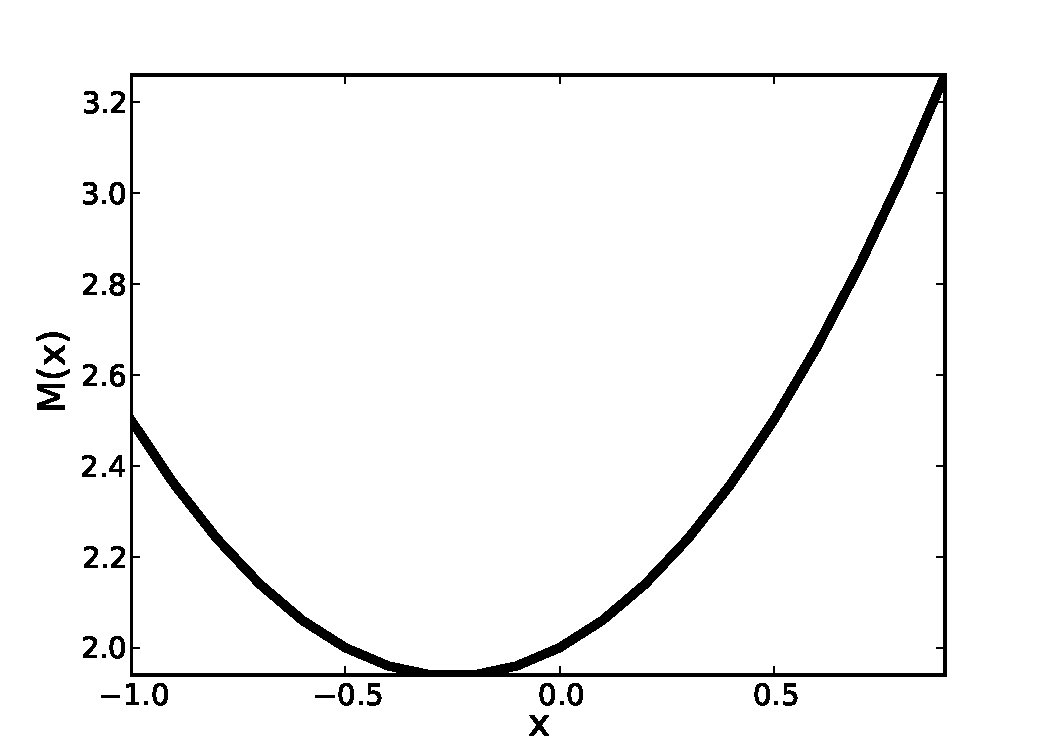
\epsfig{file=figs/mean.pdf,width=8cm}
    \caption{The mean function generated by {\sffamily `examples/mean.py'}.}
    \label{fig:mean}
\end{figure}

The mean function of a univariate Gaussian process can be interpreted as a prior guess for the GP, so it is also a univariate function. Mean functions are represented by class \code{Mean}, which is a wrapper for an ordinary \proglang{Python} function. We will use the parabolic function
\begin{equation}
    M(x) = ax^2 + bx + c.
\end{equation}

The following code (from \code{pymc/examples/gp/Mean.py}) will produce an instance of class \code{Mean} called $M$:
\begin{CodeChunk}
\begin{CodeInput}
from pymc.gp import *
def quadfun(x, a, b, c):
    return (a * x ** 2 + b * x + c)
M = Mean(quadfun, a = 1., b = .5, c = 2.)        
\end{CodeInput}
\end{CodeChunk}

The first argument of \code{Mean}'s init method is the underlying \proglang{Python} function, in this case \code{quadfun}. The extra arguments $a$, $b$  and $c$ will be memorized and passed to \code{quadfun} whenever $M$ is called; the call $M(x)$ in the plotting portion of the script does not need to pass them in.

Mean functions broadcast over their arguments in the same way as \href{http://docs.scipy.org/doc/numpy/reference/ufuncs.html}{\pkg{NumPy} universal functions} \citep{numpybook}, which means that the call $M(x)$, where $x$ is a vector, returns the vector
\begin{eqnarray*}
    [M(x_0),\ldots, M(x_{N-1})].
\end{eqnarray*}

The last part of the code plots $M(x)$ on $-1<x<1$, and its output is shown in figure \ref{fig:mean}. As expected, the plot is a parabola.

\subsection{Creating a covariance function}\label{subsub:cov}
\begin{figure}
    \centering
        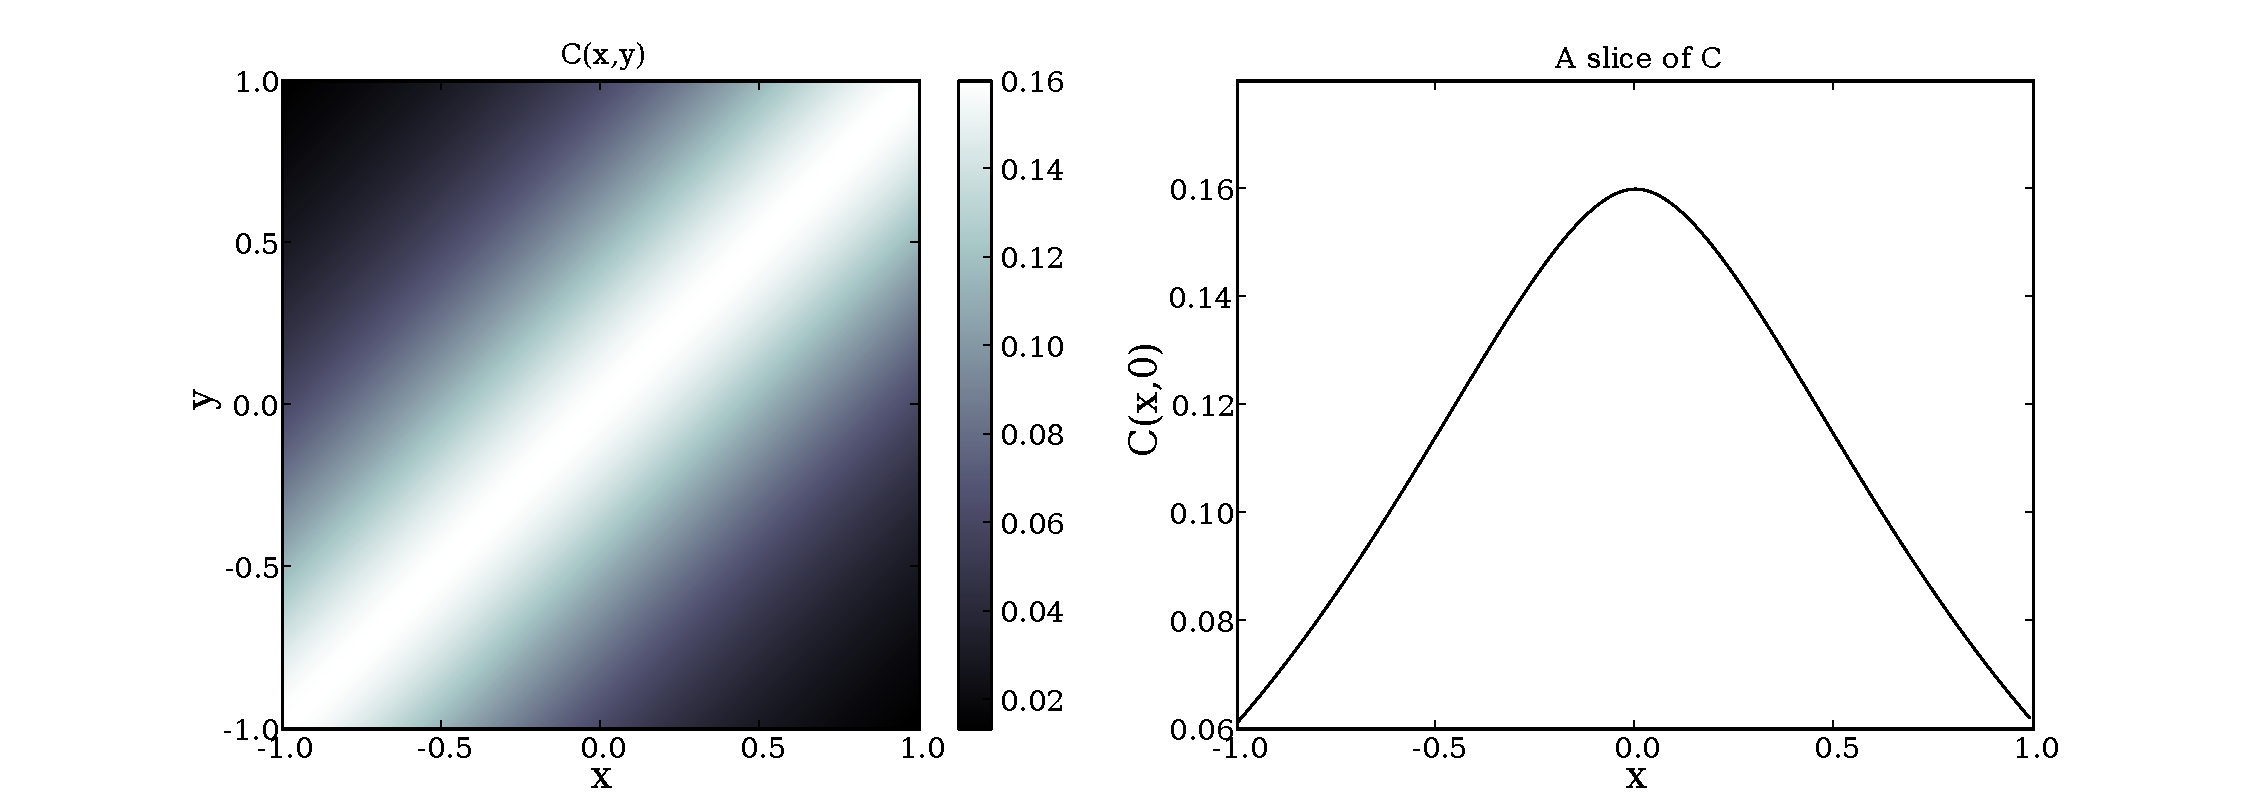
\epsfig{file=figs/cov.pdf,width=12cm}
    \caption{The covariance function generated by {\sffamily `examples/cov.py'}. On the left is the covariance function $C(x,y)$ evaluated over a square: $-1\le x\le 1,\ -1\le y\le 1$. On the right is a slice of the covariance: $C(x,0)$ for $0\le x \le 1$}
    \label{fig:cov}
\end{figure}

Gaussian process covariance functions are represented by the class \code{Covariance}, which like \code{Mean} is essentially a wrapper for ordinary \proglang{Python} functions. The example in \code{pymc/examples/gp/cov.py} uses the popular Mat\`ern covariance function \citep{banerjee}, which is provided in module \code{cov_funs}. In addition to the two arguments $x$ and $y$, the Mat\`ern covariance function takes three parameters: \code{amp} controls the amount by which realizations may deviate from their mean, \code{diff_degree} controls the roughness of realizations (the degree of differentiability), and \code{scale} controls the lengthscale over which realizations change.

The user is free to write functions to wrap in \code{Covariance} objects. See \href{http://code.google.com/p/pymc}{the package documentation} for more information.

The code in \code{pymc/examples/gp/cov.py} will produce an instance of class \code{Covariance} called $C$:
\begin{CodeChunk}
\begin{CodeInput}
from pymc.gp import *
from pymc.gp.cov_funs import matern

C = Covariance(eval_fun = matern.euclidean, diff_degree = 1.4, amp = .4, scale = 1.)
\end{CodeInput}
\end{CodeChunk}

The first argument to \code{Covariance}'s init method is the \proglang{Python} function from which the covariance function will be made. In this case, \code{eval_fun} is \code{matern.euclidean}. Covariance functions' calling conventions are slightly different from ordinary \pkg{NumPy} universal functions' \citep{numpybook} in two ways. First, broadcasting works differently. If $C$ were a \pkg{NumPy} universal function, $C(x,y)$ would return the following array:
    \begin{eqnarray*}
        \begin{array}{ccc}
            [C(x_0,y_0)& \ldots& C(x_{N-1},y_{N-1})],
        \end{array}
    \end{eqnarray*}
    where $x$ and $y$ would need to be vectors of the same length. In fact $C(x,y)$ returns a matrix:
    \begin{eqnarray*}
        \left[\begin{array}{ccc}
            C(x_0,y_0)& \ldots& C(x_0,y_{N_y-1})\\
            \vdots&\ddots&\vdots\\
            C(x_{N_x-1},y_0)& \ldots& C(x_{N_x-1},y_{N_y-1})
        \end{array}\right],
    \end{eqnarray*}
    and input arguments $x$ and $y$ don't need to be the same length. Second, covariance functions can be called with just one argument. $C(x)$ returns
    \begin{eqnarray*}
         [C(x_0,x_0)& \ldots& C(x_{N_x-1},x_{N_x-1})] = \textup{diag}(C(x,x)),
    \end{eqnarray*}
    but is computed much faster than diag$(C(x,x))$ would be.
The extra arguments \code{diff_degree, amp} and \code{scale}, which are required by \code{matern.euclidean}, will be passed to \code{matern.euclidean} by $C$ every time is called.
 
The output of \code{examples/cov.py} is shown in figure \ref{fig:cov}.

\subsubsection{Cholesky algorithms}

The numerical `heavy lifting' done by this package is primarily handled by \code{Covariance} and its subclasses. \texttt{Covariance} itself bases all its computations on the incomplete Cholesky decomposition algorithm used by the \proglang{Matlap} package \pkg{chol_incomplete} \citep{seeger}. \code{Covariance} computes rows of covariance matrices as they are needed, so if the function it wraps tends to produce covariance matrices with only a few large eigenvalues it can compute the Cholesky decomposition in less than $O(n^2)$ arithmetic operations \citep{predictivechol}.

\code{Covariance} calls back to \proglang{Python} from \proglang{Fortran} every time it needs a new row. If the function it wraps tends to produce full-rank covariance matrices (for which all rows are required), this is inefficient. \code{FullRankCovariance} is a drop-in replacement for \code{Covariance} that is much faster, but fails (with a helpful error message) if it attempts to factor a matrix that is not full rank. \code{NearlyFullRankCovariance} provides a compromise between the two: it computes covariance matrices in full in \proglang{Fortran}, then factors them using the robust algorithm of \pkg{chol_incomplete}.

\subsection{Drawing realizations}\label{subsub:realizations}
\begin{figure}
    \centering
        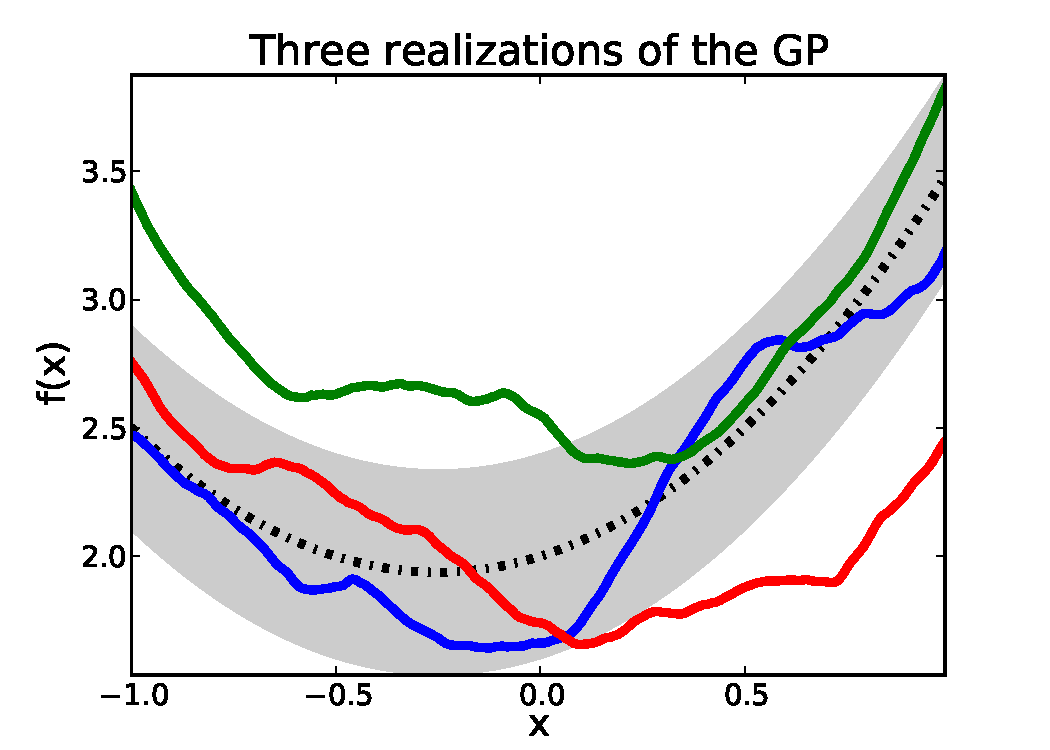
\epsfig{file=figs/realizations.pdf,width=8cm}
    \caption{Three realizations from a Gaussian process displayed with mean $\pm$ 1 sd envelope. Generated by {\sffamily `examples/realizations.py'}.}
    \label{fig:realizations}
\end{figure}

The code in \texttt{pymc/examples/gp/realizations.py} generates a list of \code{Realization} objects, which represent realizations (draws) from the Gaussian process defined by $M$ and $C$:
\begin{CodeChunk}
\begin{CodeInput}
from mean import M
from cov import C
from pymc.gp import *

f_list = [Realization(M,C) for i in range(3)]
\end{CodeInput}
\end{CodeChunk}

The init method of \code{Realization} takes only two required arguments, a \code{Mean} object and a \code{Covariance} object. Each element of \code{f_list} is a Gaussian process realization, which is essentially a randomly-generated \proglang{Python} function. Like \code{Mean} objects, \code{Realization} objects use the same broadcasting rules as \pkg{NumPy} universal functions. The call $f(x)$ returns the vector
\begin{eqnarray*}
    [f(x_0)\ldots f(x_{N-1})].
\end{eqnarray*}

Each of the three realizations in \code{f_list} is plotted in figure \ref{fig:realizations}, superimposed on a $\pm$ 1 standard deviation envelope.


\section{Nonparametric regression: observing Gaussian processes}\label{sec:observing}

\begin{figure}
    \centering
        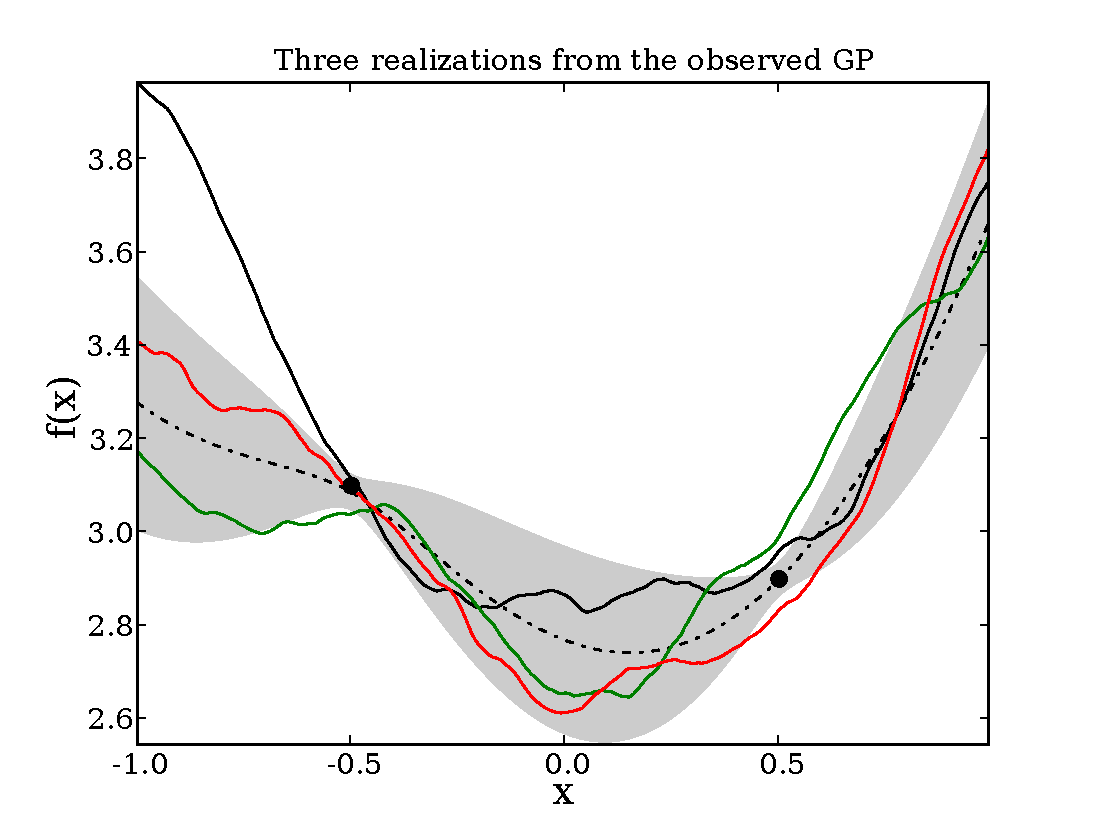
\epsfig{file=figs/obs.pdf,width=5cm}
        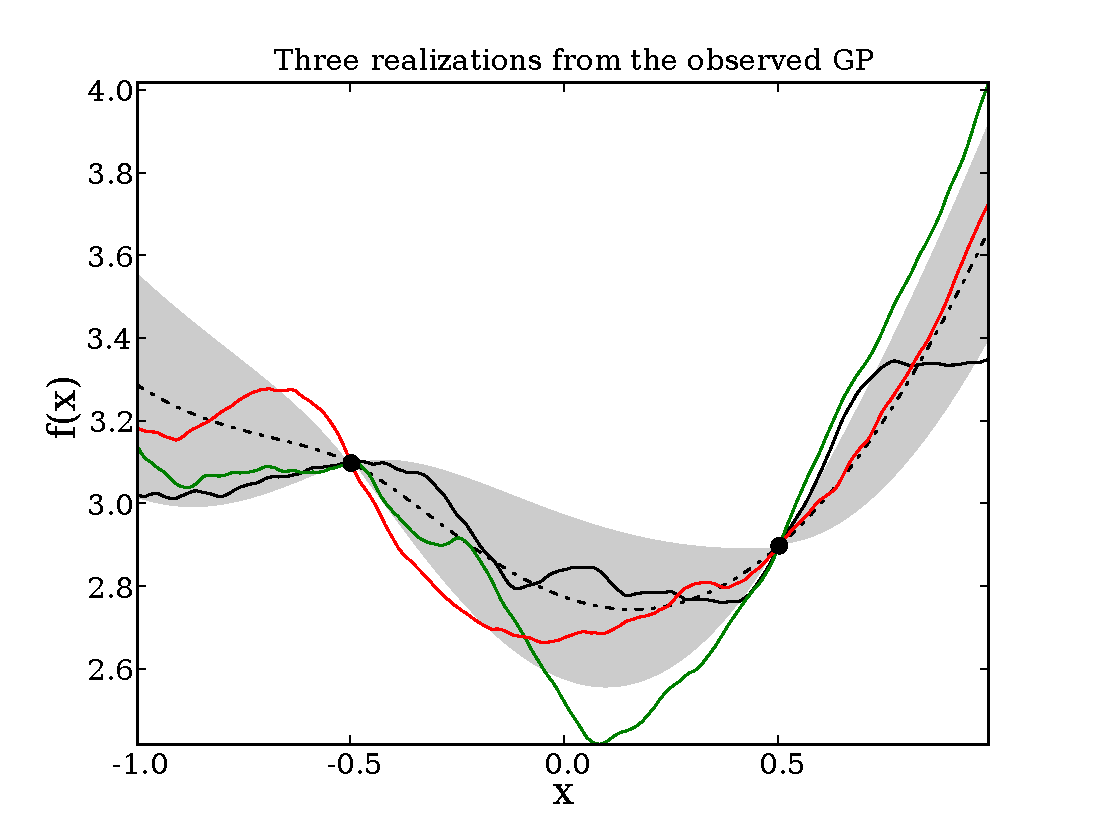
\epsfig{file=figs/cond.pdf,width=5cm}
    \caption{The output of {\sffamily `examples/observations.py'}: the observed GP with \code{obs_V = .002} (left) and \code{obs_V = 0} (right). Note that in the conditioned case, the $\pm$ 1 SD envelope shrinks to zero at the points where the observations were made, and all realizations pass through the observed values. Compare these plots to those in figure \ref{fig:realizations}.}
    \label{fig:obs}
\end{figure}

Consider the following common statistical situation: A Gaussian process prior for an unknown function $f$ is chosen, then the value of $f$ is observed at $N$ input points $[o_0\ldots o_{N-1}]$, possibly with uncertainty. If the observation error is normally distributed, it turns out that $f$'s posterior distribution given the new information is another Gaussian process, with new mean and covariance functions.

The probability model that represents this situation is as follows:
\begin{equation}
    \label{regprior}
    \left.\begin{array}{l}
        \textup{data}_i \stackrel{\tiny{\textup{ind}}}{\sim} \textup{N}(f(o_i), V_i)\\
        f \sim \textup{GP}(M,C)\\
    \end{array}\right\}\Rightarrow f|\textup{data} \sim \textup{GP}(M_o, C_o).
\end{equation}
Function \code{observe} imposes normally-distributed observations on Gaussian process distributions. This function converts $f$'s prior to its posterior by transforming $M$ and $C$ in equation \ref{regprior} to $M_o$ and $C_o$:

The code in \code{pymc/examples/gp/observation.py} imposes the observations
\begin{eqnarray*}
    f(-.5) = 3.1\\
    f(.5) = 2.9
\end{eqnarray*}
with observation variance $V=.002$ on the GP distribution defined in \code{mean.py} and \code{cov.py}:
\begin{CodeChunk}
\begin{CodeInput}
from mean import M
from cov import C
from pymc.gp import *
from numpy import *

obs_x = array([-.5,.5])
V = array([.002,.002])
data = array([3.1, 2.9])
observe(M=M, C=C, obs_mesh=obs_x, obs_V=V, obs_vals=data)

f_list = [Realization(M,C) for i in range(3)]
\end{CodeInput}
\end{CodeChunk}

The function \code{observe} takes a covariance $C$ and a mean $M$ as arguments, and essentially tells them that their realizations' values on \code{obs_mesh} have been observed to be \code{obs_vals} with variance \code{obs_V}. If \code{obs_V} is \code{None}, \code{observe} assumes that the observation variance was zero.

The output of \code{observation.py}  is shown in figure \ref{fig:obs}, along with the output with \code{obs_V=None}. Compare these to the analogous figure for the unobserved GP, figure \ref{fig:realizations}. The covariance after observation is visualized in figure \ref{fig:obscov}. The covariance `tent' has been pressed down at points where $x\approx \pm .5$ and/or $y\approx\pm .5$, which are the values where the observations were made.

\begin{figure}
    \centering
        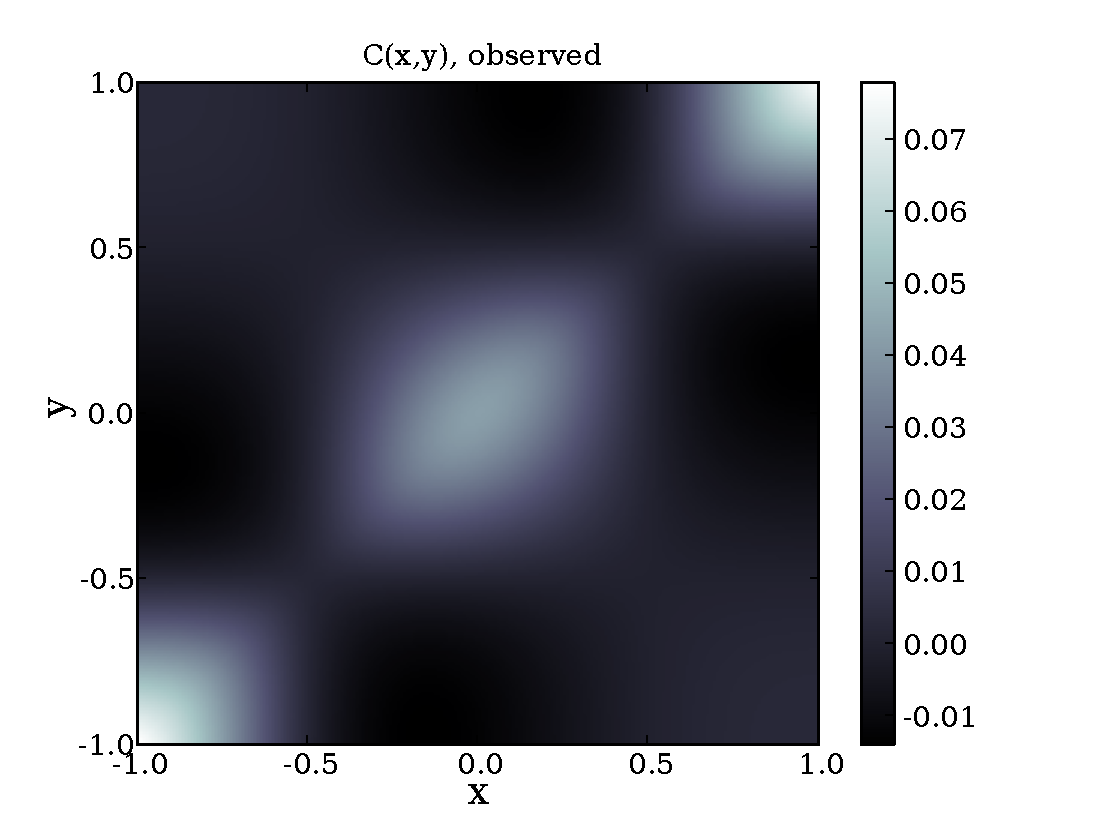
\epsfig{file=figs/obscov.pdf,width=5cm}
    \caption{The covariance function from {\sffamily `observation.py'} after observation. Compare this with the covariance function before observation, visualized in figure \ref{fig:cov} }
    \label{fig:obscov}
\end{figure}

\section{Higher-dimensional GPs}\label{sec:highdim}

In addition to functions of one variable such as $f(x)$, this package supports Gaussian process priors for functions of many variables such as $f(\mathbf{x})$, where $\mathbf{x}=[x_0\ldots x_{n-1}]$. This is useful for modeling dynamical or biological functions of many variables as well as for spatial statistics.

When array is passed into a \code{Mean}, \code{Covariance} or \code{Realization}'s init method or one of these objects is evaluated on an array, the convention is that the array's last index iterates over spatial dimension. To evaluate a covariance $C$ on the ordered pairs $(0,1)$, $(2,3)$, $(4,5)$ and $(6,7)$, the user could pass in the following two-dimensional \pkg{NumPy} array:
\begin{verbatim}
[[0,1]
 [2,3]
 [4,5]
 [6,7]]
\end{verbatim}
or the following three-dimensional array:
\begin{verbatim}
[[[0,1]
  [2,3]],

  [4,5]
  [6,7]]]
\end{verbatim}
Either is fine, since in both the last index iterates over elements of the ordered pairs.

The exception to this rule is one-dimensional input arrays. The array
\begin{verbatim}
[0, 1, 2, 3, 4, 5, 6, 7]
\end{verbatim}
is interpreted as an array of eight one-dimensional values, whereas the array
\begin{verbatim}
[[0, 1, 2, 3, 4, 5, 6, 7]]
\end{verbatim}
is interpreted as a single eight-dimensional value according to the convention above.

Means and covariances learn their spatial dimension the first time they are called or observed. Some covariances, such as those specified in geographic coordinates, have an intrinsic spatial dimension. Realizations inherit their spatial dimension from their means and covariances when possible, otherwise they infer it the first time they are called. If one of these objects is subsequently called with an input of a different dimension, it raises an error.

\subsection{Covariance function bundles and coordinate systems}
The examples so far, starting with \code{examples/cov.py}, have used the covariance function \code{matern.euclidean}. This function is an attribute of the \code{matern} object, which is an instance of class \code{covariance_function_bundle}.

Instances of \code{covariance_function_bundle} have three attributes, \code{euclidean}, \code{geo_deg} and \code{geo_rad}, which correspond to standard coordinate systems:
\begin{itemize}
    \item \code{euclidean}: $n$-dimensional Euclidean coordinates.
    \item \code{geo_deg}: Geographic coordinates (longitude, latitude) in degrees, with unit radius.
    \item \code{geo_rad}: Geographic coordinates (longitude, latitude) in radians, with unit radius.
\end{itemize}

See \href{http://code.google.com/p/pymc}{the package documentation} for information regarding creation and extension of covariance function bundles.

\section{Basis covariances}\label{sec:basis}

\begin{figure}[htbp]
    \centering
        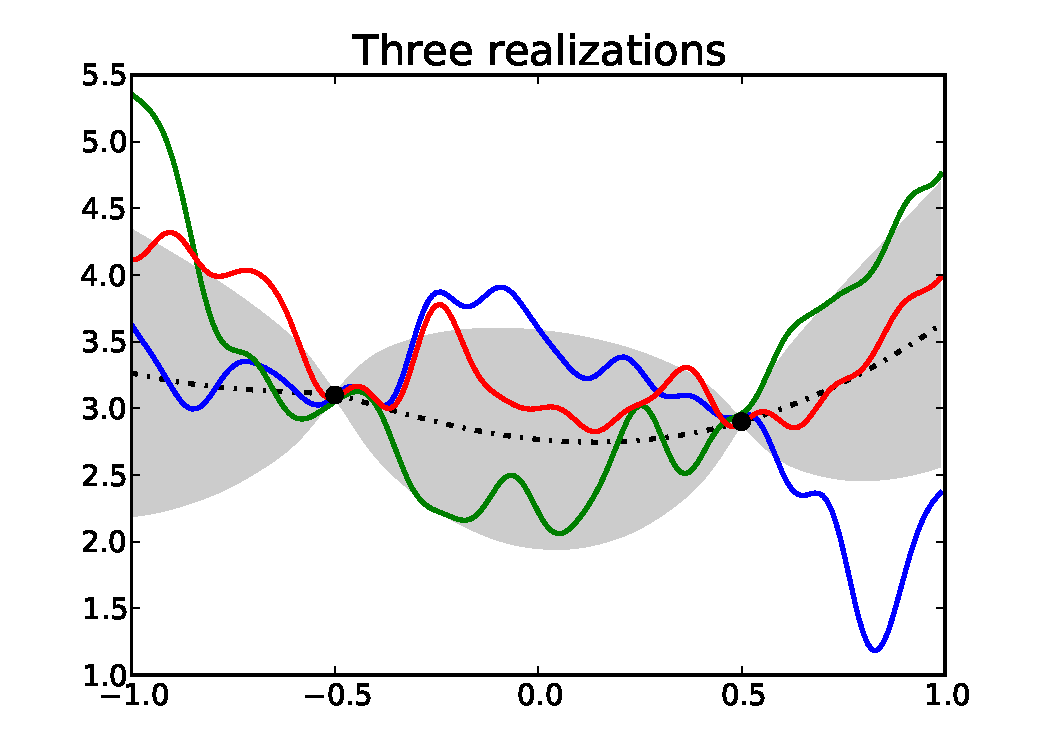
\epsfig{file=figs/basiscov.pdf,width=8cm}
        \caption{Three realizations of an observed Gaussian process whose covariance is an instance of \code{BasisCovariance}. The basis in this case is function \code{fourier_basis} from module \code{cov_funs}. 25 basis functions are used.}
    \label{fig:basiscov}
\end{figure}

It is possible to create random functions from linear combinations of finite sets of basis functions $\{e\}$ with random coefficients $\{c\}$:
\begin{eqnarray*}
    f(x) = M(x) + \sum_{i_0=0}^{n_0-1}\ldots \sum_{i_{N-1}=0}^{n_{N-1}-1} c_{i_1\ldots i_{N-1}} e_{i_1\ldots i_{N-1}}(x), \\
    \{c\}\sim \textup{N}(0,K).
\end{eqnarray*}
It follows that $f$ is a Gaussian process with mean $M$ and covariance defined by
\begin{eqnarray*}
    C(x,y)=\sum_{i_0=0}^{n_0-1}\ldots \sum_{i_{N-1}=0}^{n_{N-1}-1} \sum_{j_0=0}^{n_0-1}\ldots \sum_{j_{N-1}=0}^{n_{N-1}-1} e_{i_0\ldots i_{N-1}}(x) e_{j_0\ldots j_{N-1}}(x) K_{i_0\ldots i_{N-1}, j_0\ldots j_{N-1}},
\end{eqnarray*}
where $K$ is the covariance of the coefficients $c$.

Particularly successful applications of this general idea are:
\begin{description}
    \item[Random Fourier series:] $e_i(x) = \sin(i\pi x/L)$ or $\cos(i\pi x/L)$. See \cite{spanos}.
    \item[Gaussian process convolutions:] $e_i(x) = \exp(-(x-\mu_n)^2)$. See \cite{convolution}.
    \item[B-splines:] $e_i(x) = $ a polynomial times an interval indicator. See \href{http://en.wikipedia.org/wiki/Basis_B-spline}{Wikipedia}'s article.
\end{description}
Such representations can be very efficient when there are many observations in a low-dimensional space, but are relatively inflexible in that they generally produce realizations that are infinitely differentiable. In some applications, this tradeoff makes sense.

This package supports basis representations via the \code{BasisCovariance} class:
\begin{verbatim}
    C = BasisCovariance(basis, cov, **basis_params)
\end{verbatim}
The arguments are:
\begin{description}
    \item[\code{basis}:] Must be an array of functions, of any shape. Each basis function will be evaluated at $x$ with the extra parameters. The basis functions should obey the same calling conventions as mean functions: return values should have shape \code{x.shape[:-1]} unless $x$ is one-dimensional, in which case return values should be of the same shape as \code{x}. Note that each function should take the entire input array as an argument.
    \item[\code{cov}:] An array whose shape is either:
        \begin{itemize}
            \item Of the same shape as \code{basis}. In this case the coefficients are assumed independent, and \code{cov[i[0],...,i[N-1]]} (an $N$-dimensional index) simply gives the prior variance of the corresponding coefficient.
            \item Of shape \code{basis.shape * 2}, using \proglang{Python}'s convention for tuple multiplication. In this case \code{cov[i[0],...,i[N-1], j[0],...,j[N-1]]} (a $2N$-dimensional index) gives the covariance of $c_{i_0\ldots i_{N-1}}$ and $c_{j_1\ldots j_{N-1}}$.
        \end{itemize}
        Internally, the basis array is ravelled and this covariance tensor is reshaped into a matrix. This input convention makes it easier to keep track of which covariance value corresponds to which coefficients. The covariance tensor must be symmetric (\code{cov[i[0],...,i[N-1], j[0],...,j[N-1]]} $=$ \code{cov[j[0],...,j[N-1], i[0],...,i[N-1]]}), and positive semidefinite when reshaped to a matrix.
    \item[\code{basis_params}:] Any extra parameters required by the basis functions.
\end{description}

\section{Separable bases}

Many bases, such as Fourier series, can be decomposed into products of functions as follows:
\begin{eqnarray*}
    e_{i_0\ldots i_{N-1}}(x) = \prod_{j=0}^{N-1}e_{i_j}^j(x)
\end{eqnarray*}
Basis covariances constructed using such bases can be represented more efficiently using \code{SeparableBasisCovariance} objects. These objects are constructed just like \code{BasisCovariance} objects, but instead of an $n_0\times \ldots \times n_{N-1}$ array of basis functions they take a nested lists of functions as follows:
\begin{verbatim}
    basis = [ [e[0][0], ... ,e[0][n[0]-1]]
                       ...
              [e[N-1][0], ... ,e[N-1][n[N-1]-1]] ].
\end{verbatim}
For an $N$-dimensional Fourier basis, each of the \code{e}'s would be a sine or cosine; frequency would increase with the second index. As with \code{BasisCovariance}, each basis needs to take the entire input array \code{x} and \code{basis_params} as arguments. See \code{fourier_basis} in \code{examples/gp/basiscov.py} for an example.

\subsection{Example}

Once created, a \code{BasisCovariance} or \code{SeparableBasisCovariance} object behaves just like a \code{Covariance} object, but it and any \code{Mean} and \code{Realization} objects associated with it will take advantage of the efficient basis representation in their internal computations. An example of \code{SeparableBasisCovariance} usage is given in \code{pymc/examples/gp/basis_cov.py}. Compare its output in figure \ref{fig:basiscov} to that of \code{pymc/examples/gp/observation.py}.
 

\chapter{Incorporating Gaussian processes in PyMC probability models}\label{cha:PyMC}
This chapter will show you how to build and fit statistical models that go beyond simple nonparametric regression.
\chapter{Incorporating Gaussian processes in larger probability models with PyMC}\label{cha:PyMC}
This chapter will show you how to build and fit statistical models that go beyond simple nonparametric regression.

\section{Gaussian process submodels}

\subsection{The \texttt{GaussianProcess} class} 

\section{Step methods}
Some general ideas
\subsection{The \texttt{GPEvaluationGibbs} class} 
\subsection{Step methods that handle parents of Gaussian processes}
\subsubsection{Choosing a mesh}  



\section{Example: A simple extension of nonparametric regression}\label{sub:BasicMCMC}
The files \file{examples/gp/PyMCModel.py} and \file{examples/gp/MCMC.py} show Gaussian process submodels and the step methods listed above in action. The probability model created by \file{PyMCModel.py} is illustrated as a directed acyclic graph in figure \ref{fig:unobservedModel}. If you comment the last line, $f_eval$ will be handled by a default \class{GPParentAdaptiveMetropolis} instance. If you leave it uncommented, $f$ will be handled by a \class{GPEvaluationGibbs} instance.

The main script \file{examples/gp/MCMC.py} is mostly devoted to plotting, and its output is shown in figure \ref{fig:MCMCOutput} for both the \class{GPEvaluationMetropolis} and \class{GPParentAdaptiveMetropolis} step methods.

\begin{figure}
    \centering
        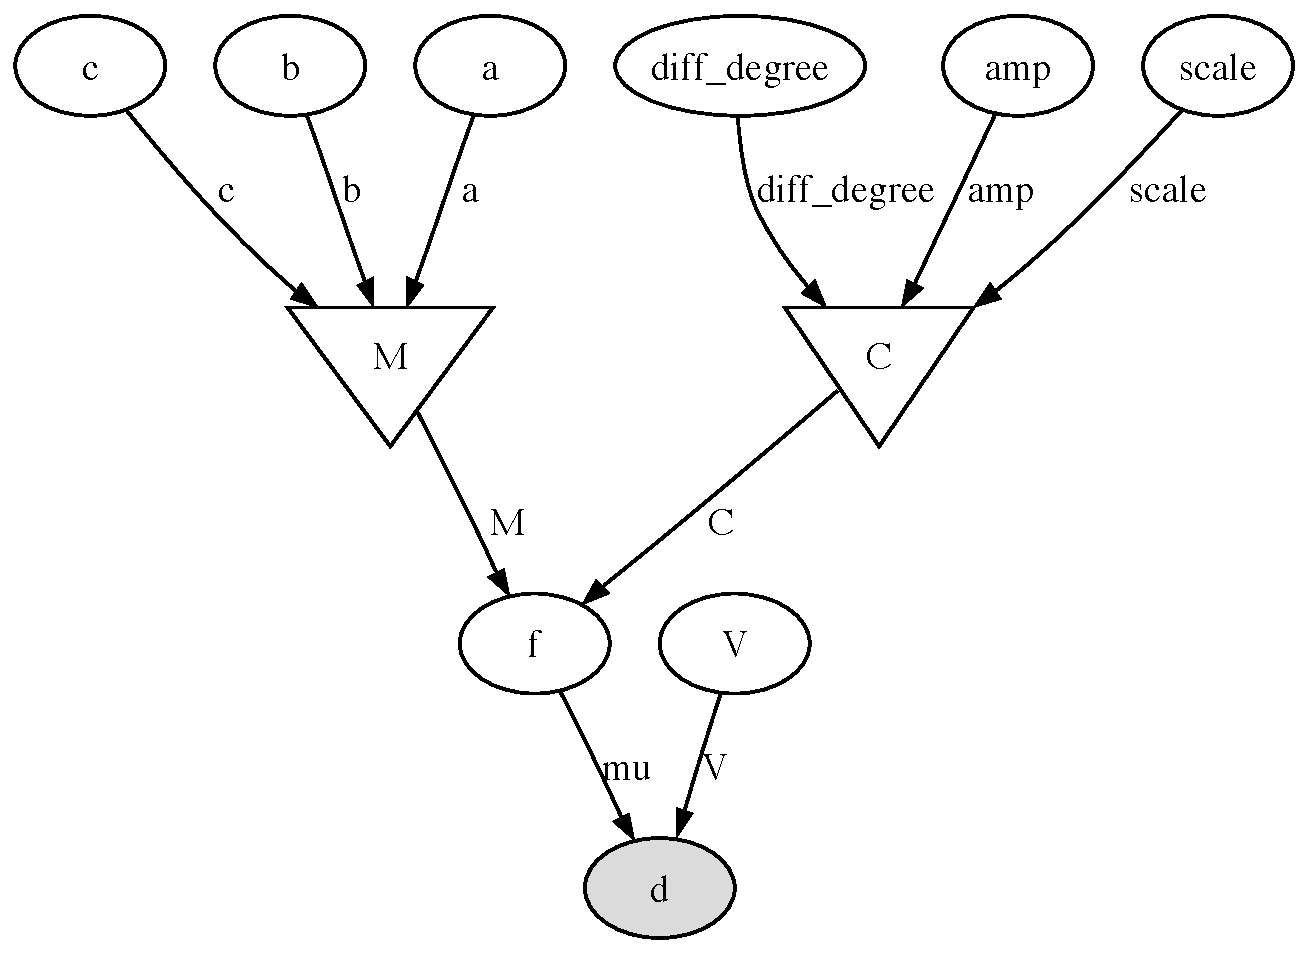
\epsfig{file=figs/unobservedModel.pdf, width=10cm}
    \caption{The PyMC-generated directed acyclic graph representation of the extended nonparametric regression model created by \textsf{`examples/gp/PyMCModel.py'} . Ellipses represent \class{Stochastic} objects (variables whose values are unknown even if their parents' values are known), triangles represent \class{Deterministic} objects (variables whose values can be determined if their parents' values are known), and rectangles represent \class{Stochastic} objects with the \member{isdata} flag set to \member{True} (data). Arrows point from parent to child, and arrow labels show the name assigned to the parent by the child. For instance, \class{C} considers \class{C_amp} to be its `\class{amp}' parameter.}
    \label{fig:unobservedModel}
\end{figure}

\begin{figure}
    \centering
        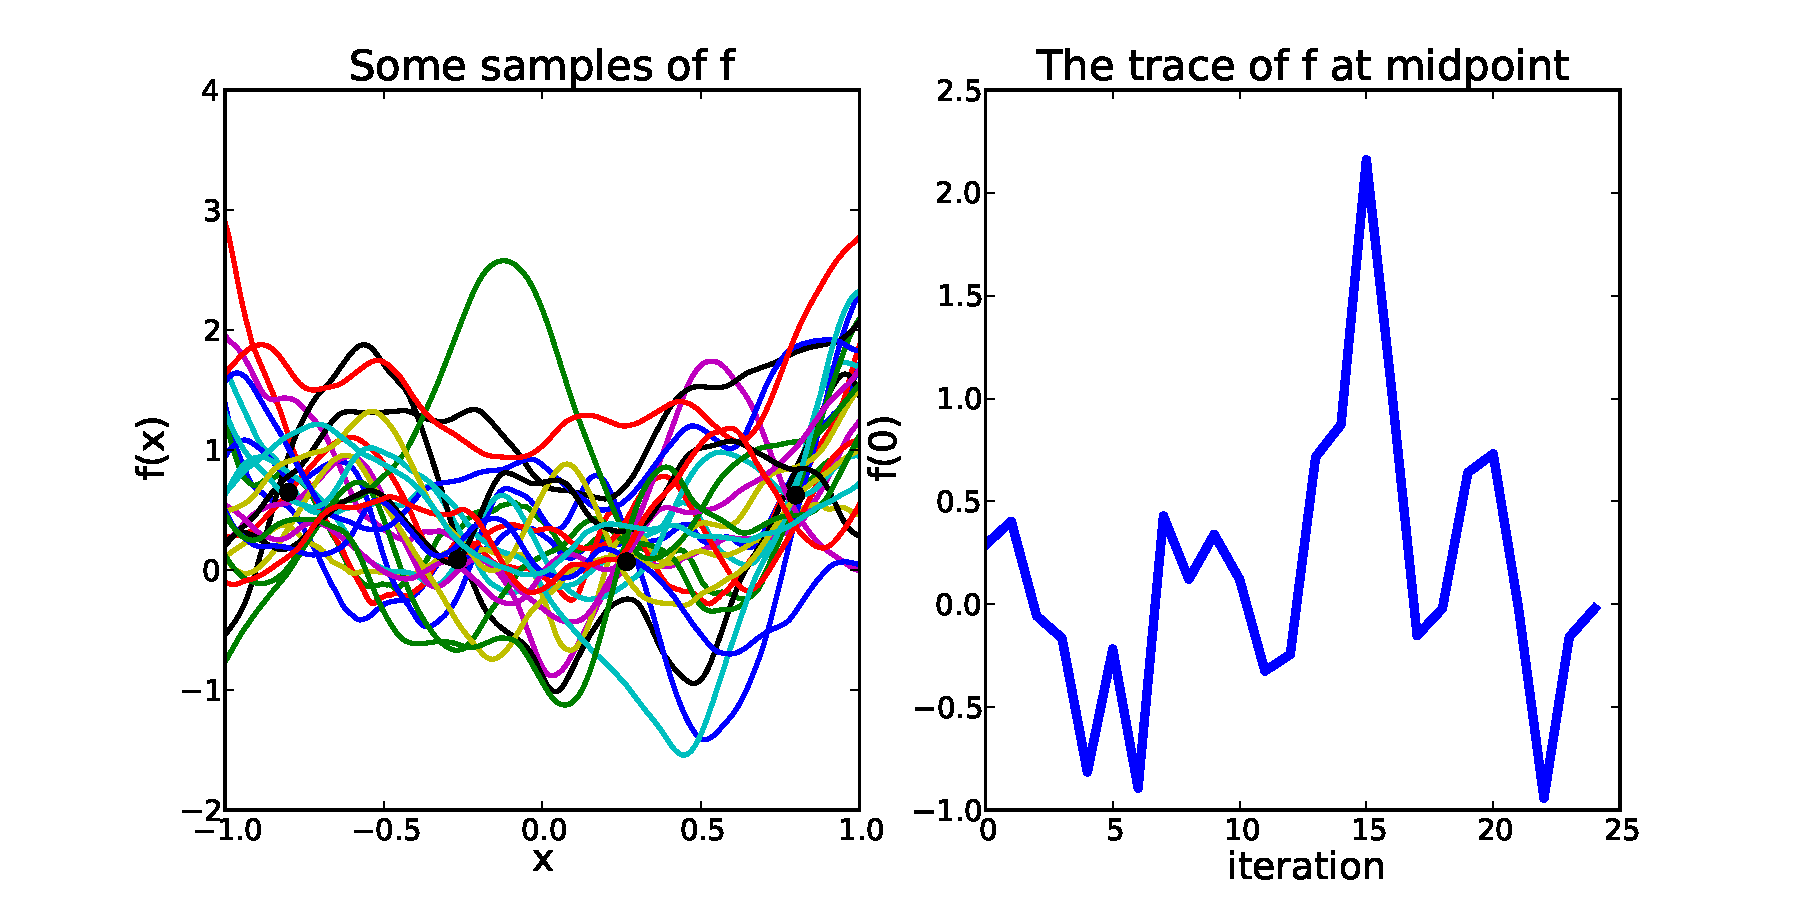
\epsfig{file=figs/gibbsSamples.pdf,width=10cm}
        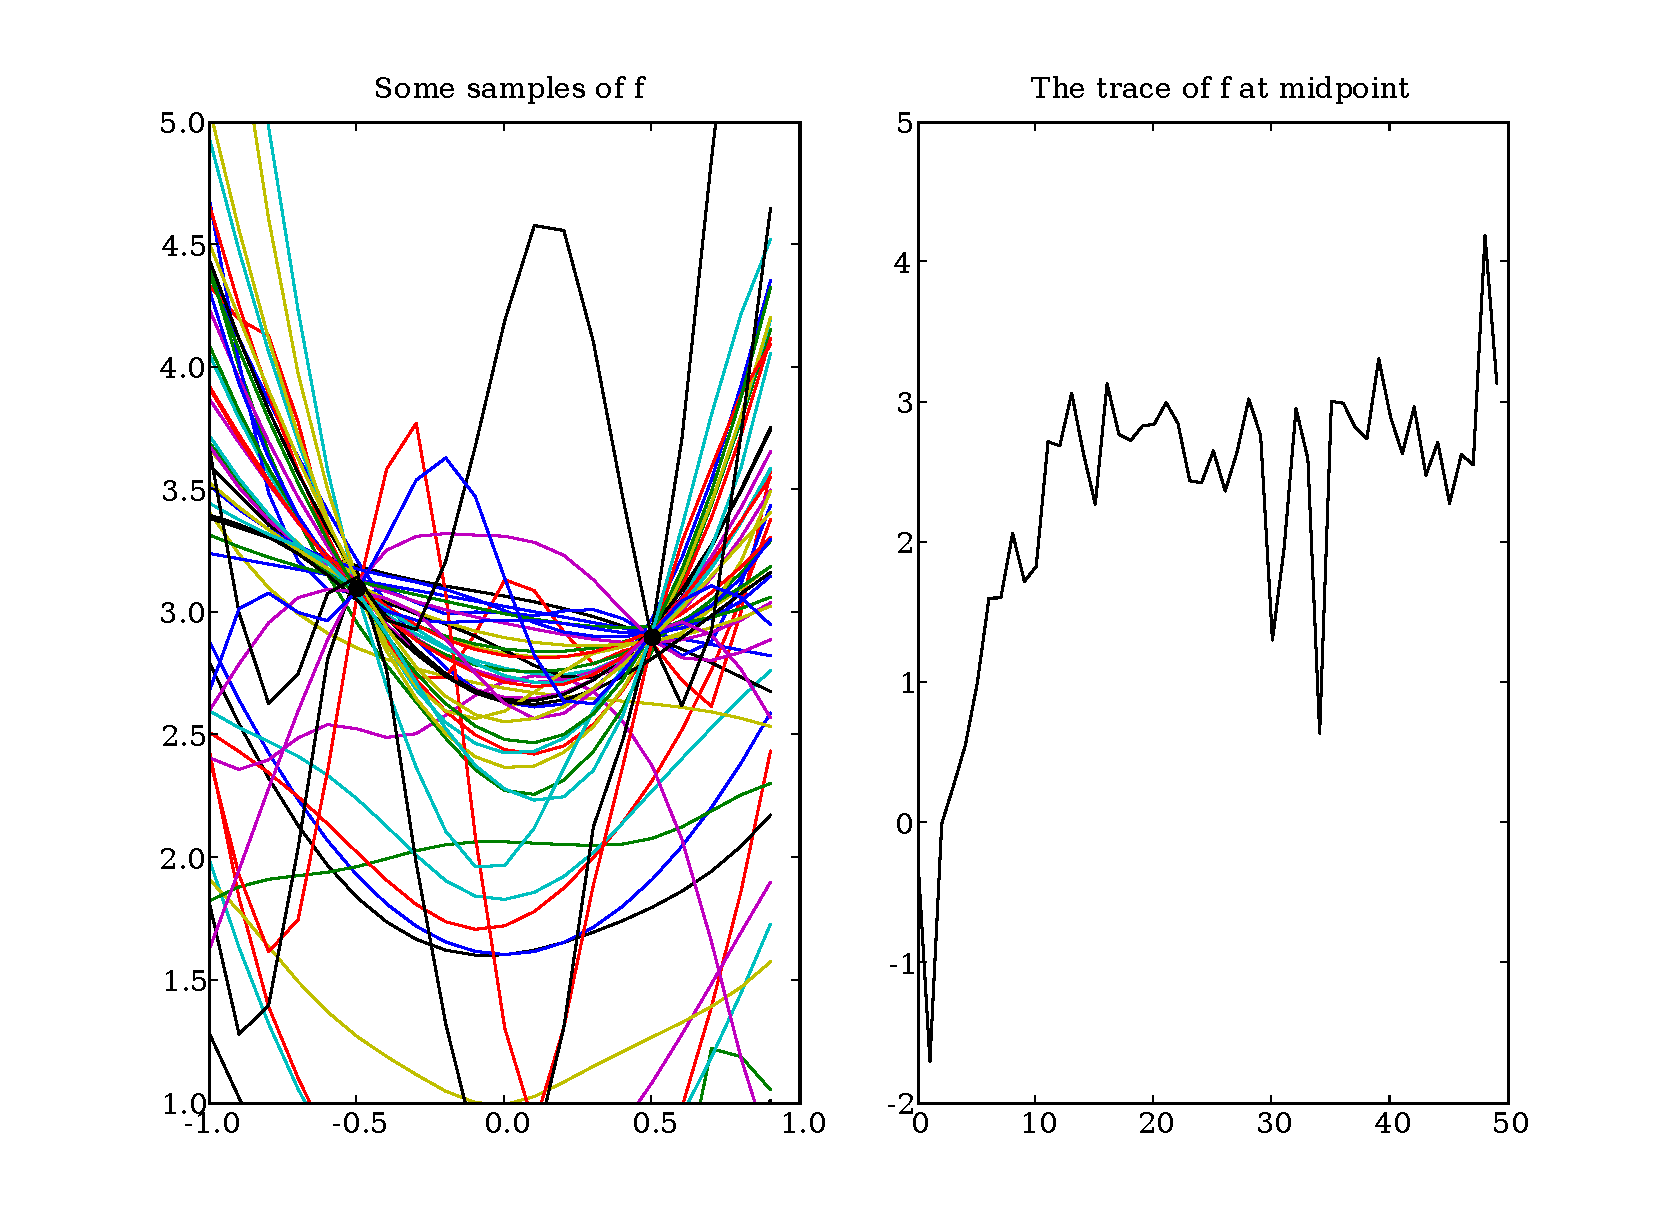
\epsfig{file=figs/metroSamples.pdf,width=10cm}
    \caption{The output of {\sffamily `examples/gp/MCMC.py'} using the \class{GPEvaluationGibbs} (top) and \class{GPParentAdaptiveMetropolis} (bottom) step methods. Note that the Metropolis samples take several iterations to `burn in' to their dense support, whereas the Gibbs samples jump there more or less immediately.
    \label{fig:MCMCOutput}
\end{figure}

\section{Example: Munch, Kottas and Mangel's stock-recruitment study}\label{sub:MMKMCMC}

\begin{figure}
    \centering
        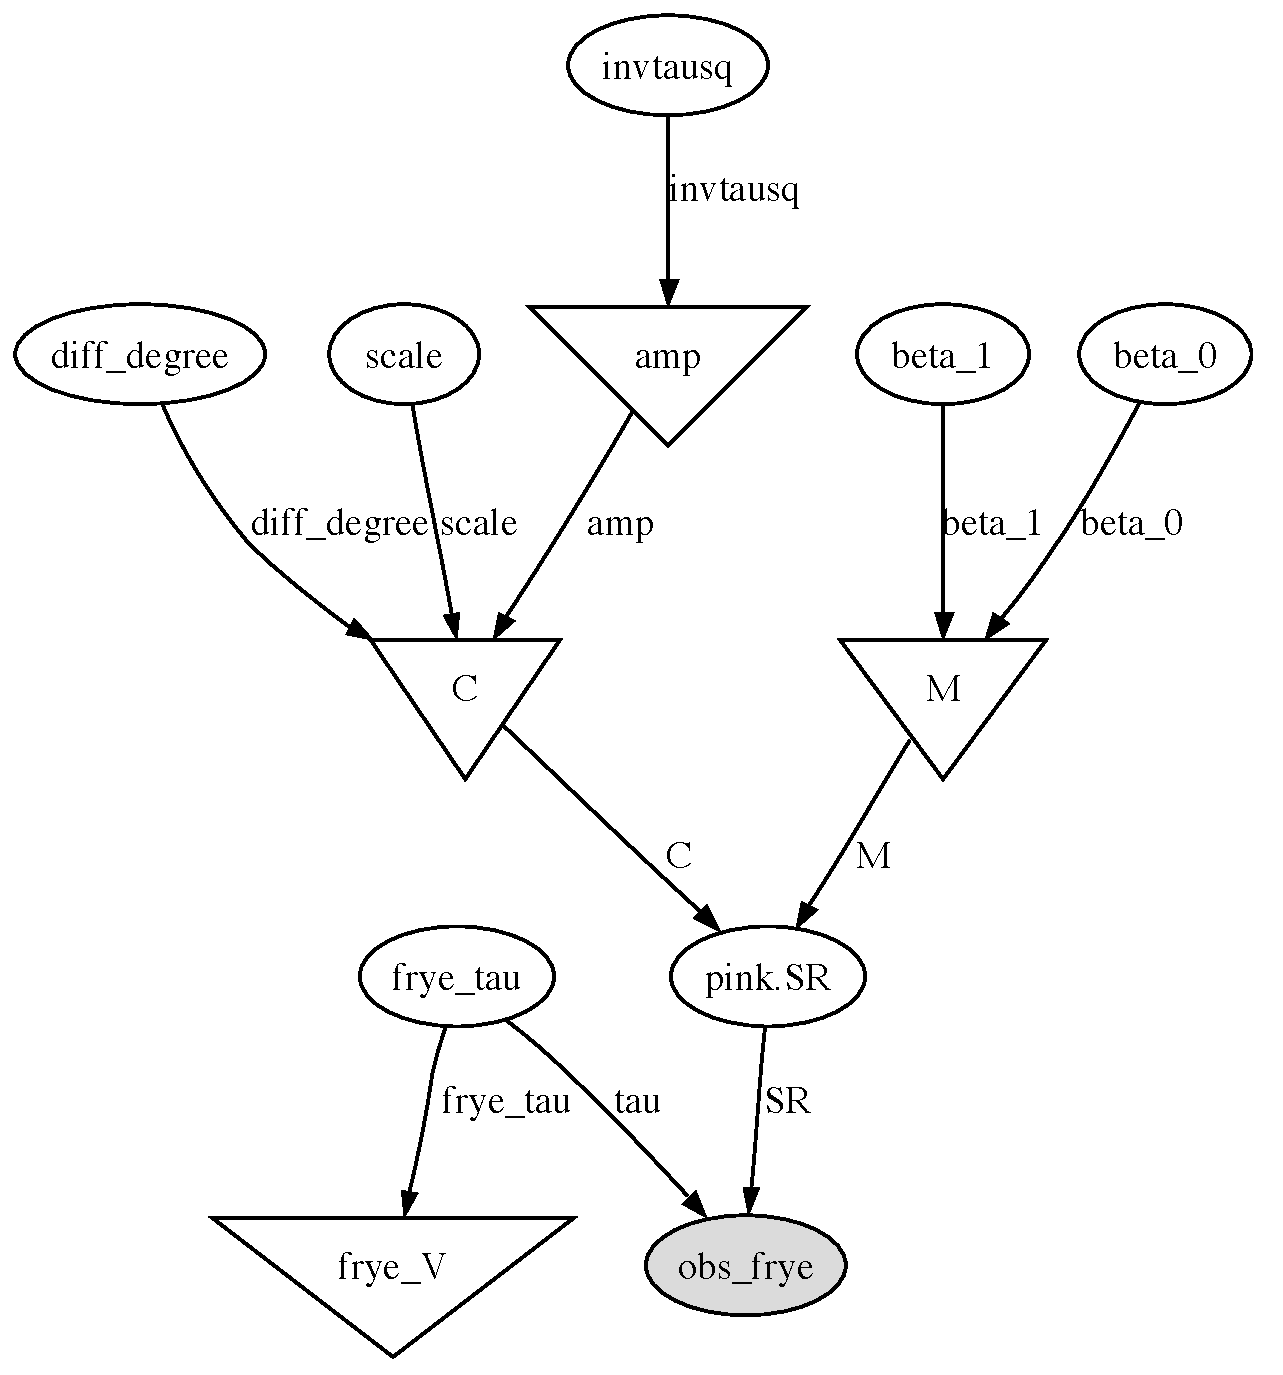
\epsfig{file=figs/MKMsalmon.pdf, width=10cm}
    \caption{A PyMC-generated directed acyclic graph representation of the probability model in (\ref{eqn:MMKModel}), which is implemented in file \textsf{`examples/gp/more_examples/MKMSalmon/salmon_sampler.py'}. A very similar probability model was used by Munch, Kottas and Mangel to infer stock-recruitment functions for three salmonid species. The label `\texttt{pink.SR}' indicates that this particular model corresponds to the pink salmon (\emph{Onchorhynchus gorbuscha}) data. Note that two coordinate transformations are implemented using PyMC deterministic variables. This technique can help lazy programmers avoid transforming priors by hand, and in less trivial cases it can save computation by caching the transformed parameters.}
    \label{fig:MMKsalmonmodel}
\end{figure}

\begin{figure}
    \centering
        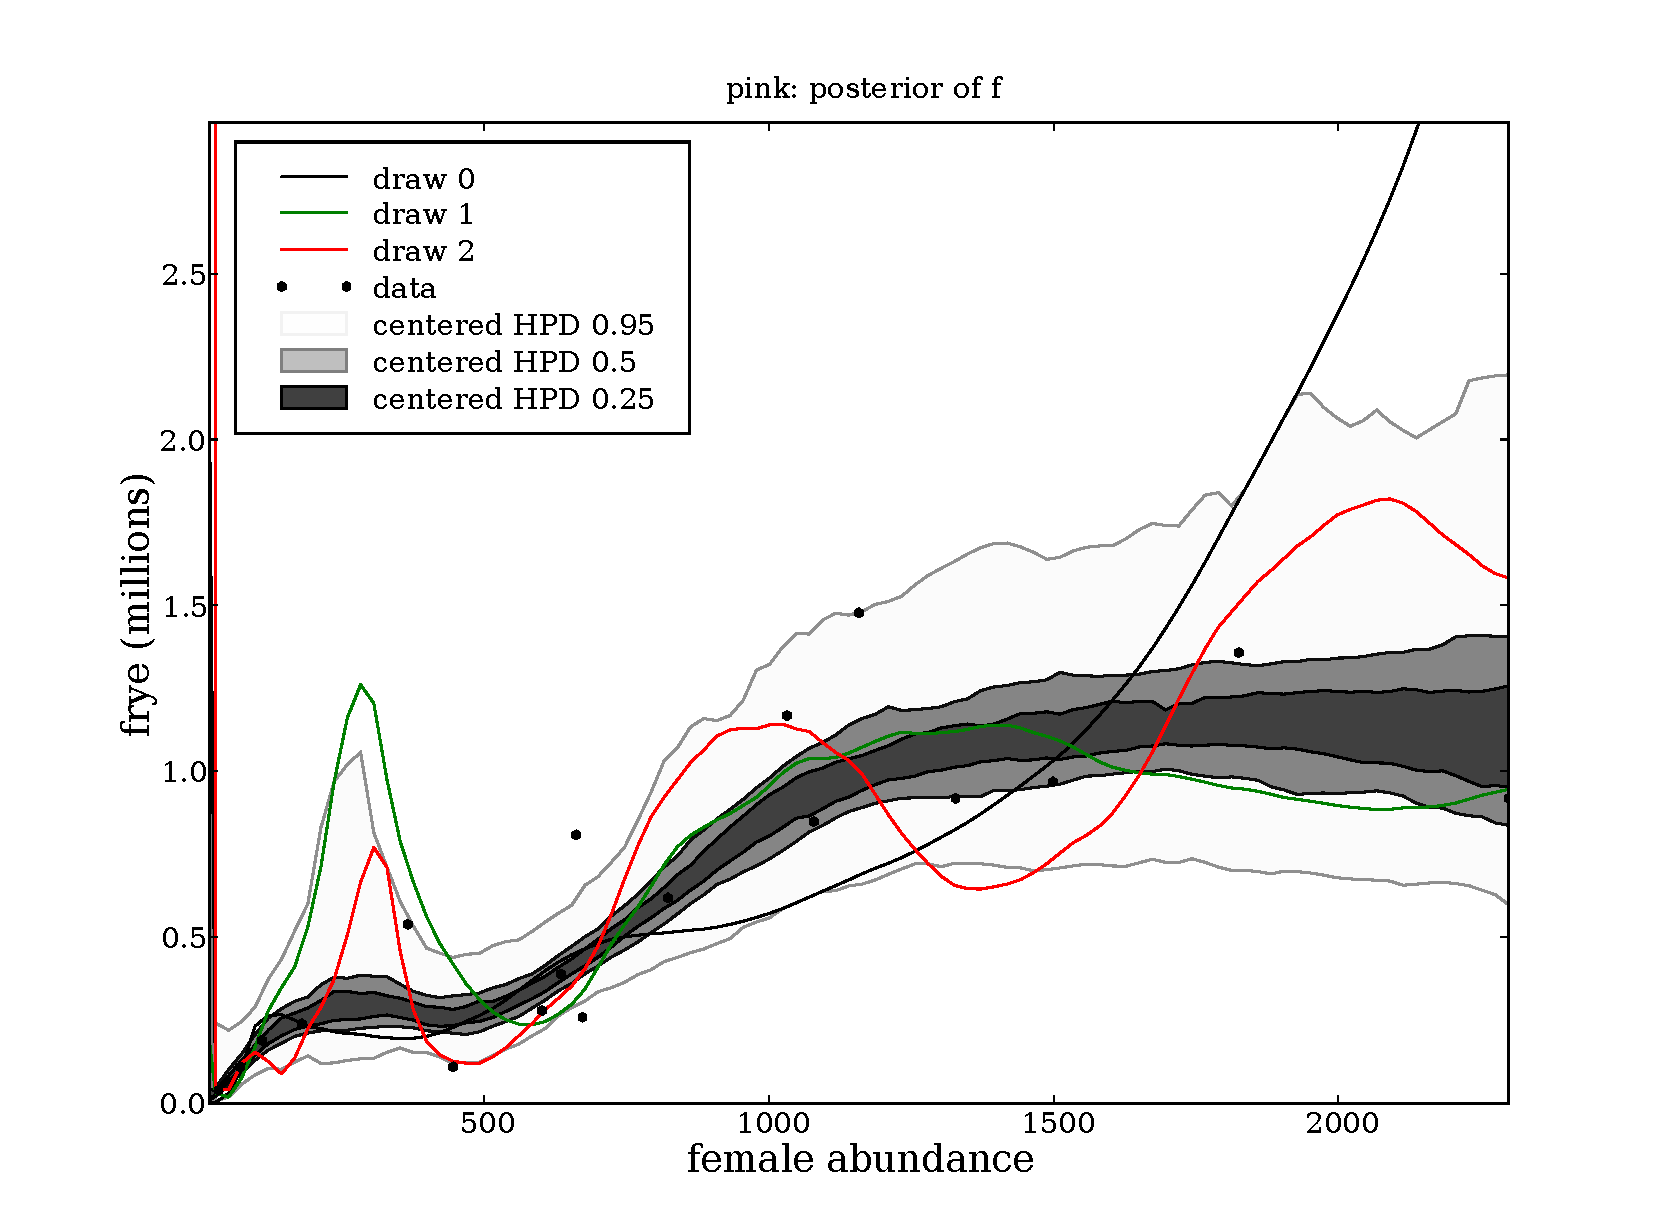
\epsfig{file=figs/pinkfpost.pdf, width=10cm}
    \caption{The posterior of the stock-recruitment function for pink salmon (\emph{Onchorhynchus gorbuscha}). The data are shown as heavy black dots. The centered 95\%, 50\% and 25\% posterior probability intervals are shown as shaded regions. Three draws from the posterior are plotted.}
    \label{fig:pinkfpost}
\end{figure}

\begin{figure}
    \centering
        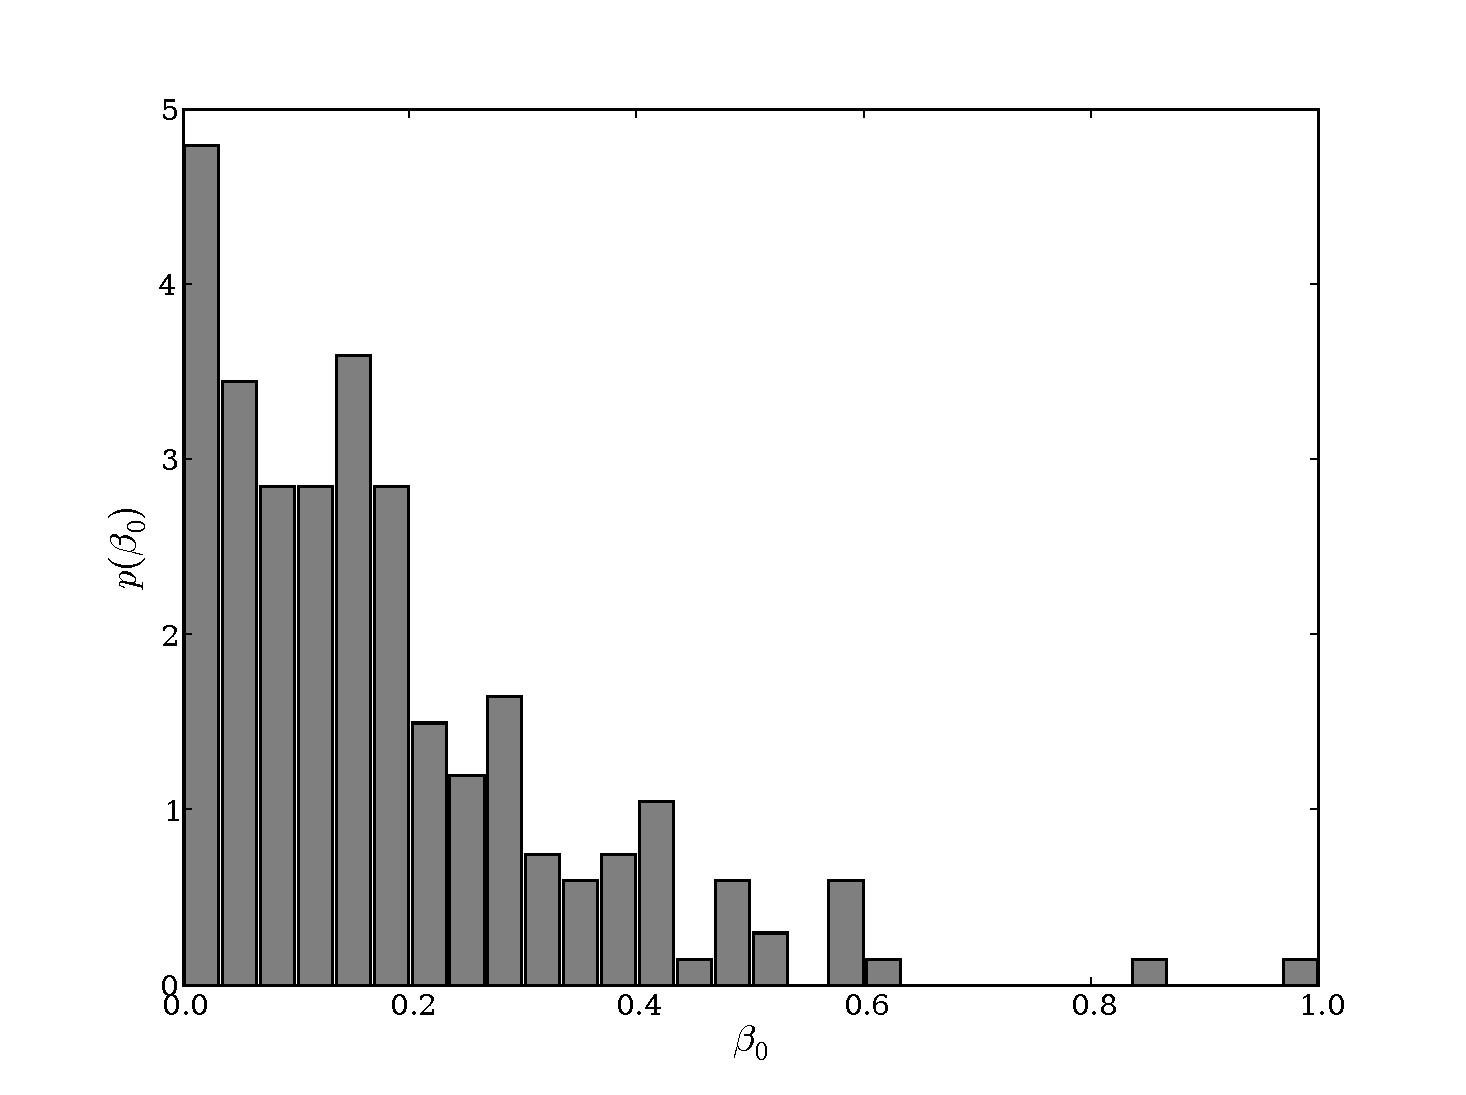
\epsfig{file=figs/pinkbeta0post.pdf, width=5cm}
        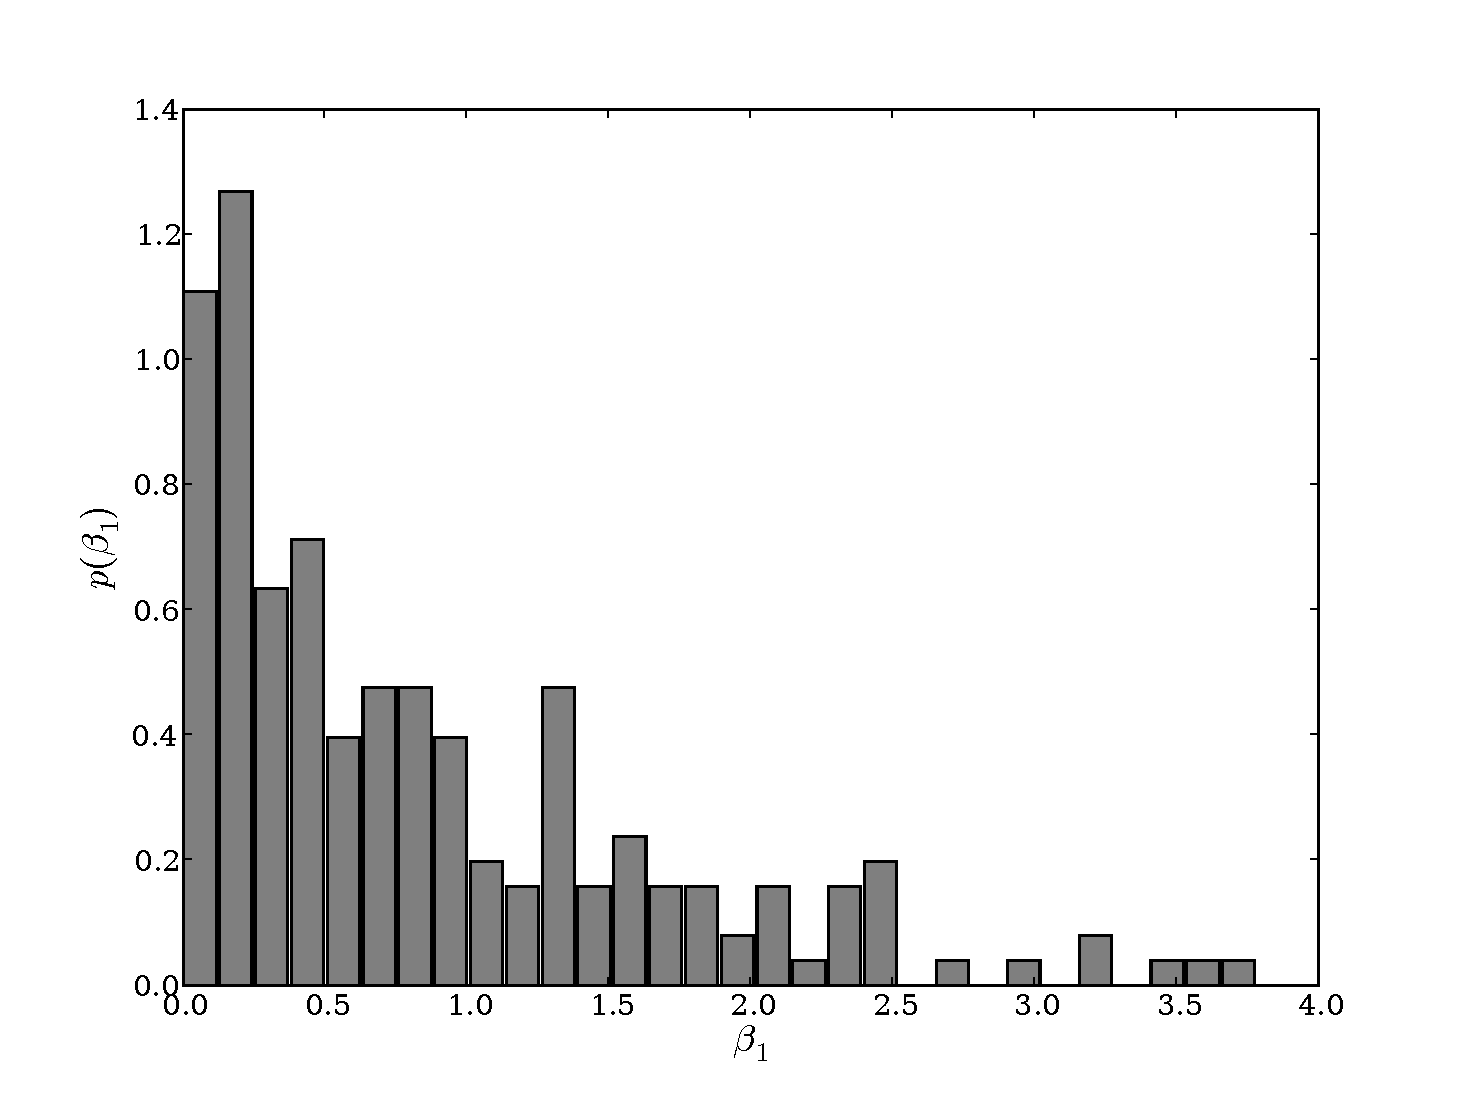
\epsfig{file=figs/pinkbeta1post.pdf, width=5cm}
        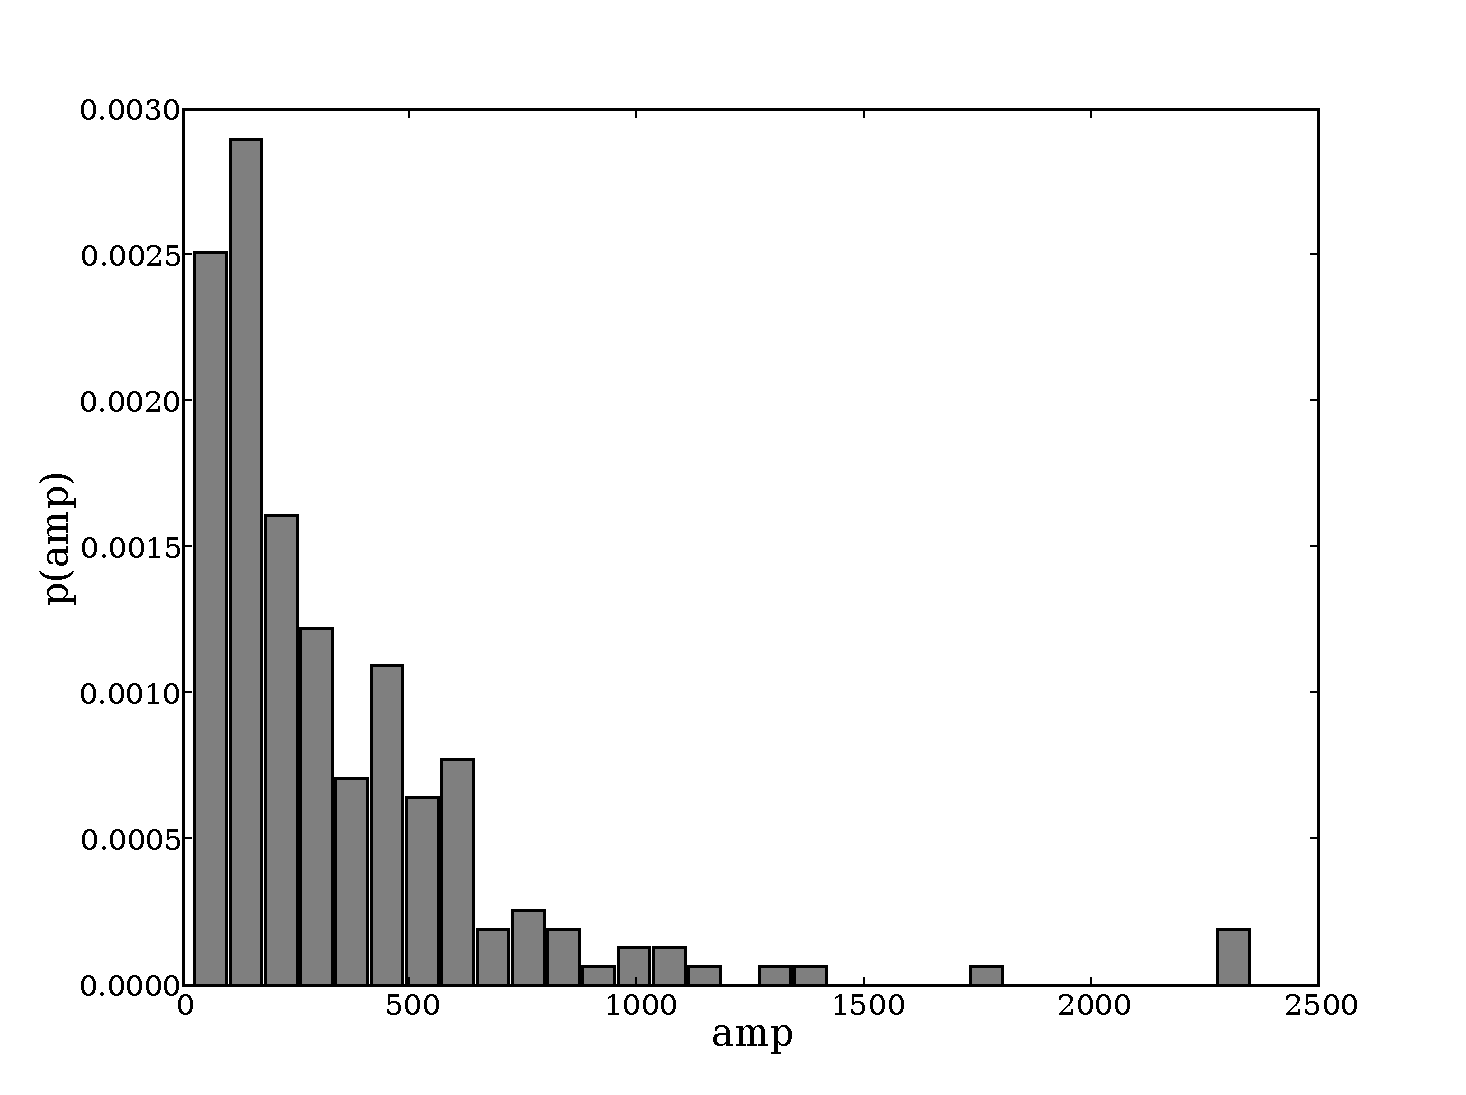
\epsfig{file=figs/pinkamppost.pdf, width=5cm}
        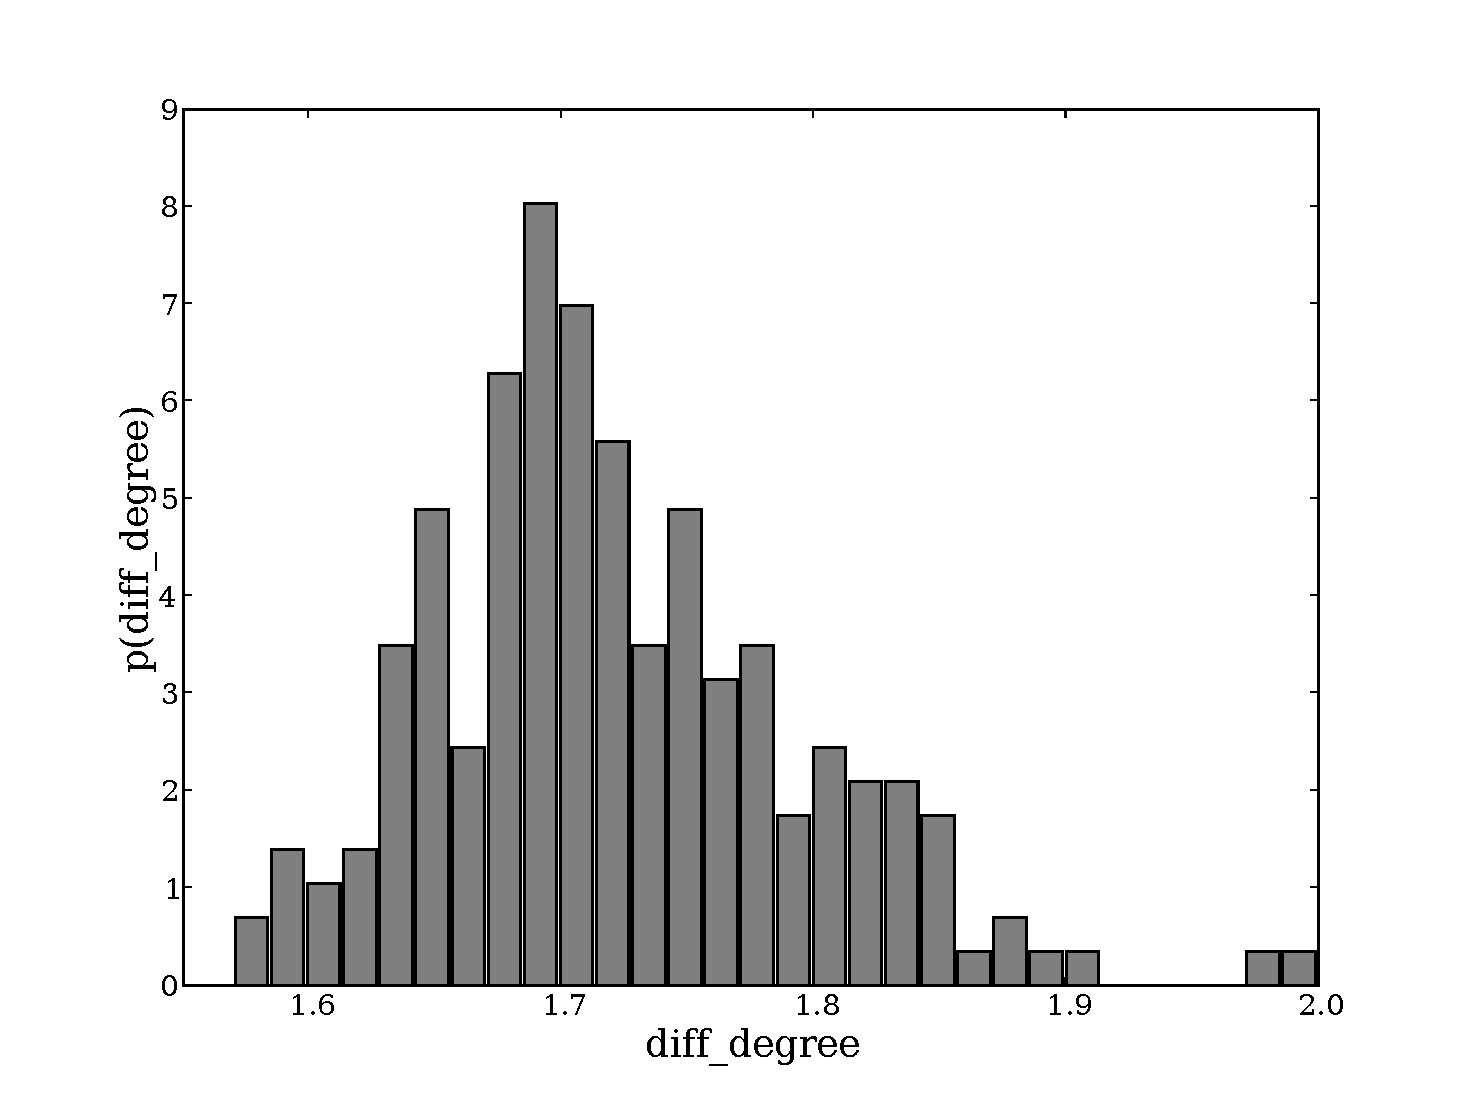
\epsfig{file=figs/pinkdiffdegreepost.pdf, width=5cm}
        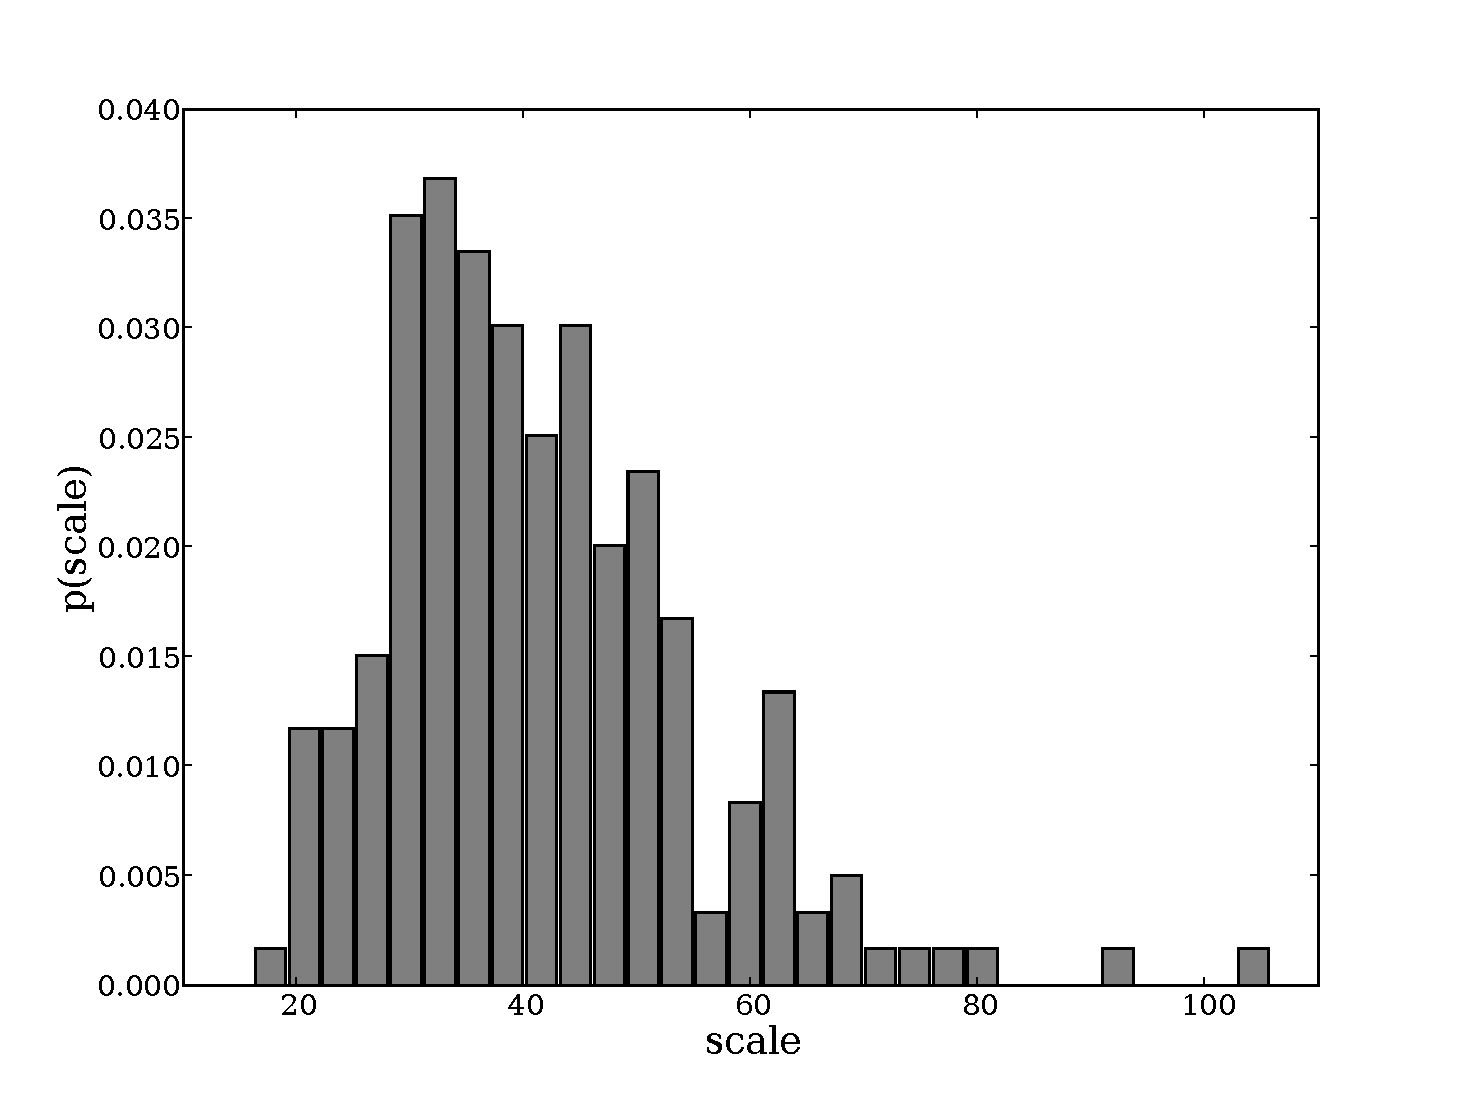
\epsfig{file=figs/pinkscalepost.pdf, width=5cm}
        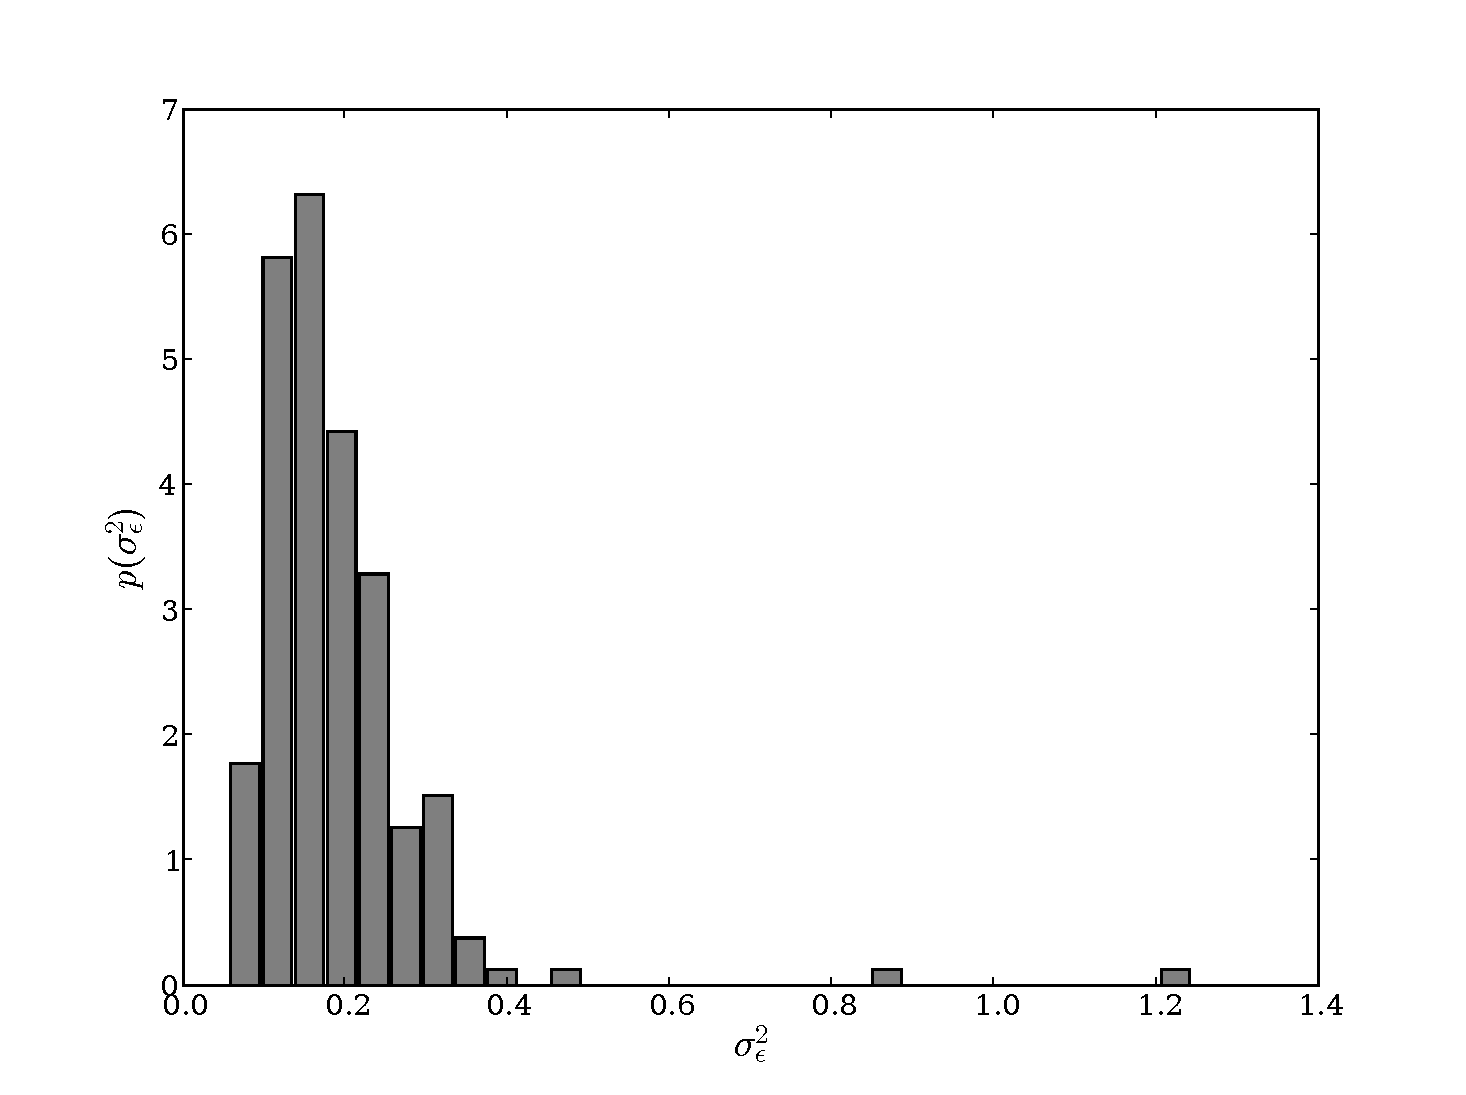
\epsfig{file=figs/pinkVpost.pdf, width=5cm}
    \caption{The marginal posterior distributions of the mean and covariance parameters of the stock-recruitment function for pink salmon (\emph{Onchorhynchus gorbuscha}).}
    \label{fig:pinkparams}
\end{figure}

We now have the tools to duplicate Munch, Kottas and Mangel's \cite{mmk} stock-recruitment results. The full probability we'll use follows. It is like Munch, Kottas and Mangel's probability model, but we will use a Mat\`ern covariance function. Here \texttt{SR} is the stock-recruitment function, C is its covariance and M is its mean.
\begin{equation}
    \label{eqn:MMKModel}
    \begin{array}{ll}
        \texttt{frye}[i] \stackrel{\tiny{\textup{ind}}}{\sim} \textup{N}(exp(\mathtt{SR}(\log(\mathtt{abundance}[i]))), V),& i=1\ldots n\\
        \texttt{SR}\sim \textup{GP}(M,C)& \\
        M:x\rightarrow \beta_0+\beta_1 \log(x)&\\
        C:x,y\rightarrow \texttt{matern.euclidean}(x,y;\ \texttt{diff_degree},\texttt{amp},\texttt{scale})&\\
        V,\ \beta_0,\ \beta_1,\ \texttt{diff_degree},\ \texttt{amp},\ \texttt{scale} \sim \texttt{priors}.&
    \end{array}
\end{equation}
The `priors' can be found by reading their paper (except the prior on \texttt{diff_degree}, which I chose based on what seems reasonable to me) or by reading the file \file{examples/more_examples/MMKSalmon/salmon_sampler.py}. This file contains a PyMC \class{MCMC} subclass called \class{SalmonSampler}, which reads in the data, creates a probability model incorporating the data, and provides some plotting methods.

Note that this model differs from the model in section \ref{sub:MMKregression} in that we're putting a Gaussian process prior on the stock-recruitment function in log-log space, so conditioning its value at zero isn't an option.

The probability model \class{SalmonSampler} creates is visualized as a directed acyclic graph in figure \ref{fig:MMKsalmonmodel}. Munch, Kottas and Mangel specify priors for $\texttt{amp}^{-2}$ and $V^{-1}$, and I've used PyMC deterministic variables to conveniently implement the transformations rather than changing variables manually. The posterior distribution of \texttt{SR} for the pink salmon (\emph{Onchorhynchus gorbuscha}) is shown in figure \ref{fig:pinkfpost}, and the posterior of the mean and covariance parameters for the same species are shown in figure \ref{fig:pinkparams}.


\chapter{Old stuff} 

\section{The \class{GP} class}
\class{GP} is a subclass of the PyMC \class{Stochastic} class whose value attribute is a \class{Realization} instance. Its init method takes the following arguments:
\begin{description}
    \item[$M$:] A mean object or mean-valued deterministic variable.
    \item[$C$:] A covariance object or covariance-valued deterministic variable.
    \item[\texttt{mesh=None}:] An array or an array-valued variable.
    \item[\texttt{init_mesh_vals=None}:] An optional vector of initial values for the value attribute's evaluation on \texttt{mesh}.
    \item[\texttt{mesh_eval_isdata=False}:] If \texttt{True}, the value attribute's evaluation on \texttt{mesh} is fixed at \texttt{init_mesh_vals}.
    \item[\texttt{doc, name, trace, cache_depth, verbose}:] Optional arguments that are passed directly to \code{Stochastic.\_\_init\_\_}. See PyMC's documentation.
\end{description}

\texttt{GP} instances have a log-probability attribute like any PyMC stochastic variable, but there is an important difference: If the value attribute is a realization called $f$, the log-probability attribute gives $p(f\texttt{(mesh))}|M,C)$. In other words, the log-probability attribute only cares about $f$'s evaluation on \texttt{mesh}. The reason is simple: it would be expensive and difficult to assign something like a log-density to entire realizations in most cases.

\section{The \class{GPMetropolis} and \class{GPParentMetropolis} step methods}

The a price of the `cop-out' of computing \texttt{GP}s' log-probabilities based only on their evaluation on a mesh is that the Metropolis-Hastings algorithm doesn't apply. \texttt{GPMetropolis} and \texttt{GPParentMetropolis} employ a strategy that will be described informally here.

Although they're contained in the same object, think about splitting the value $f$ of a \texttt{GP} into two pieces: an array $f$\texttt{(mesh)}, and a function $\tilde f$ defined on all values not in \texttt{mesh}. Denote the parents of the \class{GP} by $P$ and the children by $K$.

\section{GPMetropolis}
The Metropolis-Hastings acceptance ratio for a proposed value $f_p$ can be written as follows:
\begin{eqnarray*}
    \frac{p(K|\tilde f_p, f_p(\mathtt{mesh}))\ p(\tilde f_p|f_p(\mathtt{mesh}), P)\ p(f_p(\mathtt{mesh}) | P)\ q(\tilde f|f(\mathtt{mesh}))\ q(f(\mathtt{mesh}))}{p(\mathtt{K}|\tilde f, f(\mathtt{mesh}))\ p(\tilde f|f(\mathtt{mesh}), P)\ p(f(\mathtt{mesh}) | P)\ q(\tilde f_p|f(\mathtt{mesh}))\ q(f_p(\mathtt{mesh}))},
\end{eqnarray*}
where $q$ denotes proposal densities. We want to avoid computing all terms with $\tilde f$ or $\tilde f_p$ in the consequent position:
\begin{eqnarray*}
    p(\tilde f_p|f_p(\texttt{mesh}), P),\\ q(\tilde f|f(\texttt{mesh})),\\ p(\tilde f|f(\texttt{mesh}), P),\\ q(\tilde f_p|f(\texttt{mesh})),
\end{eqnarray*}
but all other terms are fine. We can make these terms cancel by choosing our proposal distribution as follows:
\begin{eqnarray*}
    q(\tilde f_p|f(\texttt{mesh})) = p(\tilde f_p|f_p(\texttt{mesh}), P).
\end{eqnarray*}
In other words, if we propose $\tilde f$ from its prior distribution conditional on $f(\texttt{mesh})$ and its parents whenever we propose $f(\texttt{mesh})$, we don't have to worry about computing the intractable terms. This is what \class{GPMetropolis} does.

\class{GPMetropolis} reports its competence to handle \texttt{GP} instances as \texttt{3}, so it will be chosen as the default handler. Its init method takes the following arguments:
\begin{description}
    \item[\texttt{stoch}:] The \class{GPMetropolis} instance to be handled.
    \item[\texttt{scale=.1}:] $f(\texttt{mesh})$ will be proposed from a random-walk multivariate normal distribution with covariance equal to \texttt{C(mesh, mesh * scale * adaptive_scale_factor)}, where C is the covariance-valued parent and \texttt{adaptive_scale_factor} is the adaptive scaling factor, which is updated when \texttt{self.tune()} is called.
    \item[\texttt{verbose = 0}:] An integer from 0 to 3 indicating the preferred verbosity level.
\end{description}

\section{GPParentMetropolis}
Similarly, the Metropolis-Hastings acceptance ratio for a proposed value $P_p$ of the parents \emph{and} a proposed value $\tilde f_p$ for the function off the mesh is as follows:
\begin{eqnarray*}
    \frac{p(K|\tilde f_p)\ p(\tilde f_p|f(\texttt{mesh}), P_p)\ p(f(\texttt{mesh}) | P_p)\ q(\tilde f_p|f(\texttt{mesh}),f_p, P_p)\ q(P)}{p(K|\tilde f)\ p(\tilde f|f(\texttt{mesh}), P)\ p(f(\texttt{mesh}) | P)\ q(\tilde f_p|f(\texttt{mesh}),f)\ q(P_p)}
\end{eqnarray*}
By choosing the same proposal distribution for $\tilde f$ as above, we again avoid having to compute the intractable terms. In other words, every time a value is proposed for a \class{GP}'s parent, a value must be proposed for the \class{GP}  conditional on its value's evaluation on its mesh, and the prior probability of the \class{GP}'s children must be included in the acceptance ratio.

To implement this strategy, \class{GPParentMetropolis} wraps an instance of a \class{Metropolis} subclass. It replaces its host class's \texttt{propose} and \texttt{reject} methods with special methods that call the host's native methods, and then propose and reject values for $\tilde f$ conditional on \texttt{f(mesh)}. \class{GPParentMetropolis} also adds the \texttt{GP}'s children to its host method's children, so that the likelihood term $p(K|\tilde f)$ is included in the acceptance ratio.

\class{GPParentMetropolis} reports its competence to handle parents of \class{GP} instances as \texttt{3}, so it will be chosen as the default handler. However, its init method will choose the host method by checking the step method registry for a method that would be competent to handle the parent if it had ordinary children. Its init method takes the following arguments:
\begin{description}
    \item[\texttt{stochastic}:] The stochastic variable to handle. Must be a parent of a \class{GP} instance.
    \item[\texttt{scale = 1.}:] This parameter will be passed to the host method's init method.
    \item[\texttt{verbose = 0}:] An integer from 0 to 3 indicating the preferred verbosity level.
\end{description}

This scheme works if $K$ depends on $P$ and if $P$ has children other than the \class{GP}, though these possibilites aren't included in the rejection ratio above.

\section{Choosing a mesh} A useful mental model for these step methods is as follows: The mesh points of a \class{GP} instance are the points where you `grab' its value to propose it. If the variable's mesh is \texttt{None}, its value will be proposed from its prior, and rejection rates are likely to be quite large. If the mesh is too dense, on the other hand, computation of the log-probability will be expensive (it scales as the cube of the number of points in the mesh). If the mesh is so dense that \texttt{C(mesh, mesh)} is numerically singular, an error will be raised in the init method. This continuum is illustrated in figure \ref{fig:meshpropose}. Finding the happy medium will require some experimentation.

Another important point to bear in mind is that if the \texttt{GP}'s children depend on its value only via its evaluation on the mesh, the likelihood terms $p(K|\tilde f_p)$ and $p(K|\tilde f)$ will cancel. In other words, if the mesh is chosen so that $p(K|f)=p(K|f(\texttt{mesh}))$ then the proposed value of $\tilde f$ will have no bearing on the acceptance probability of the proposed value of \texttt{f(mesh)} or of the parents P. Such a mesh choice will generally improve the acceptance rate.

\begin{figure}
    \centering
        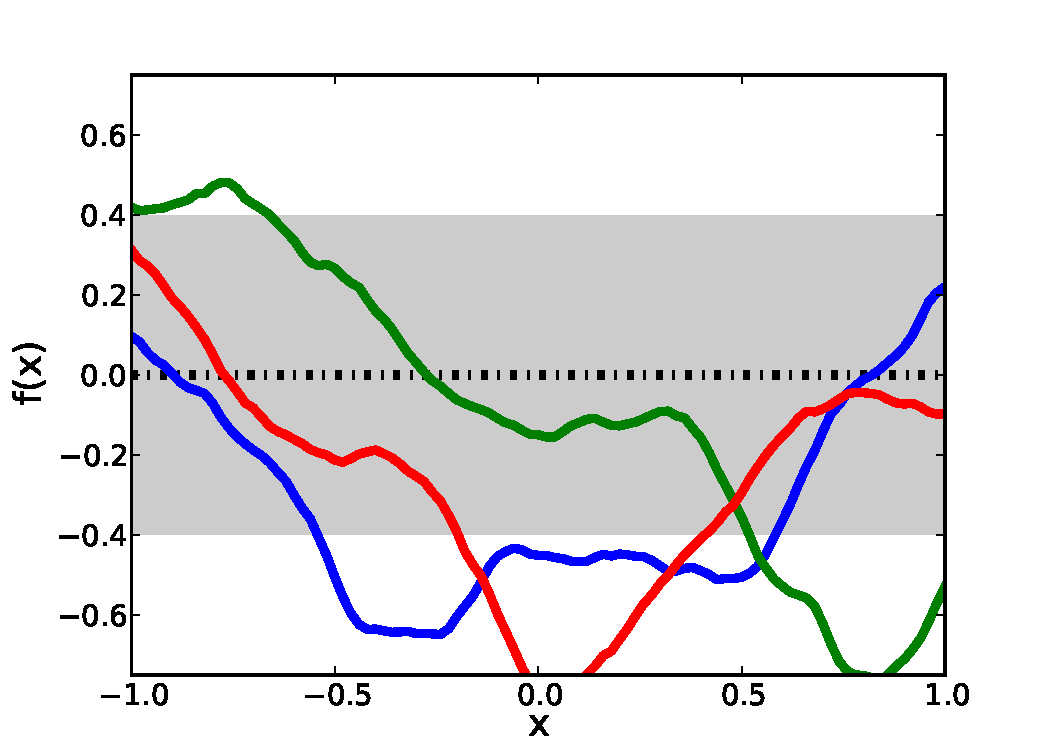
\epsfig{file=figs/nomeshpropose.pdf,width=9cm}
        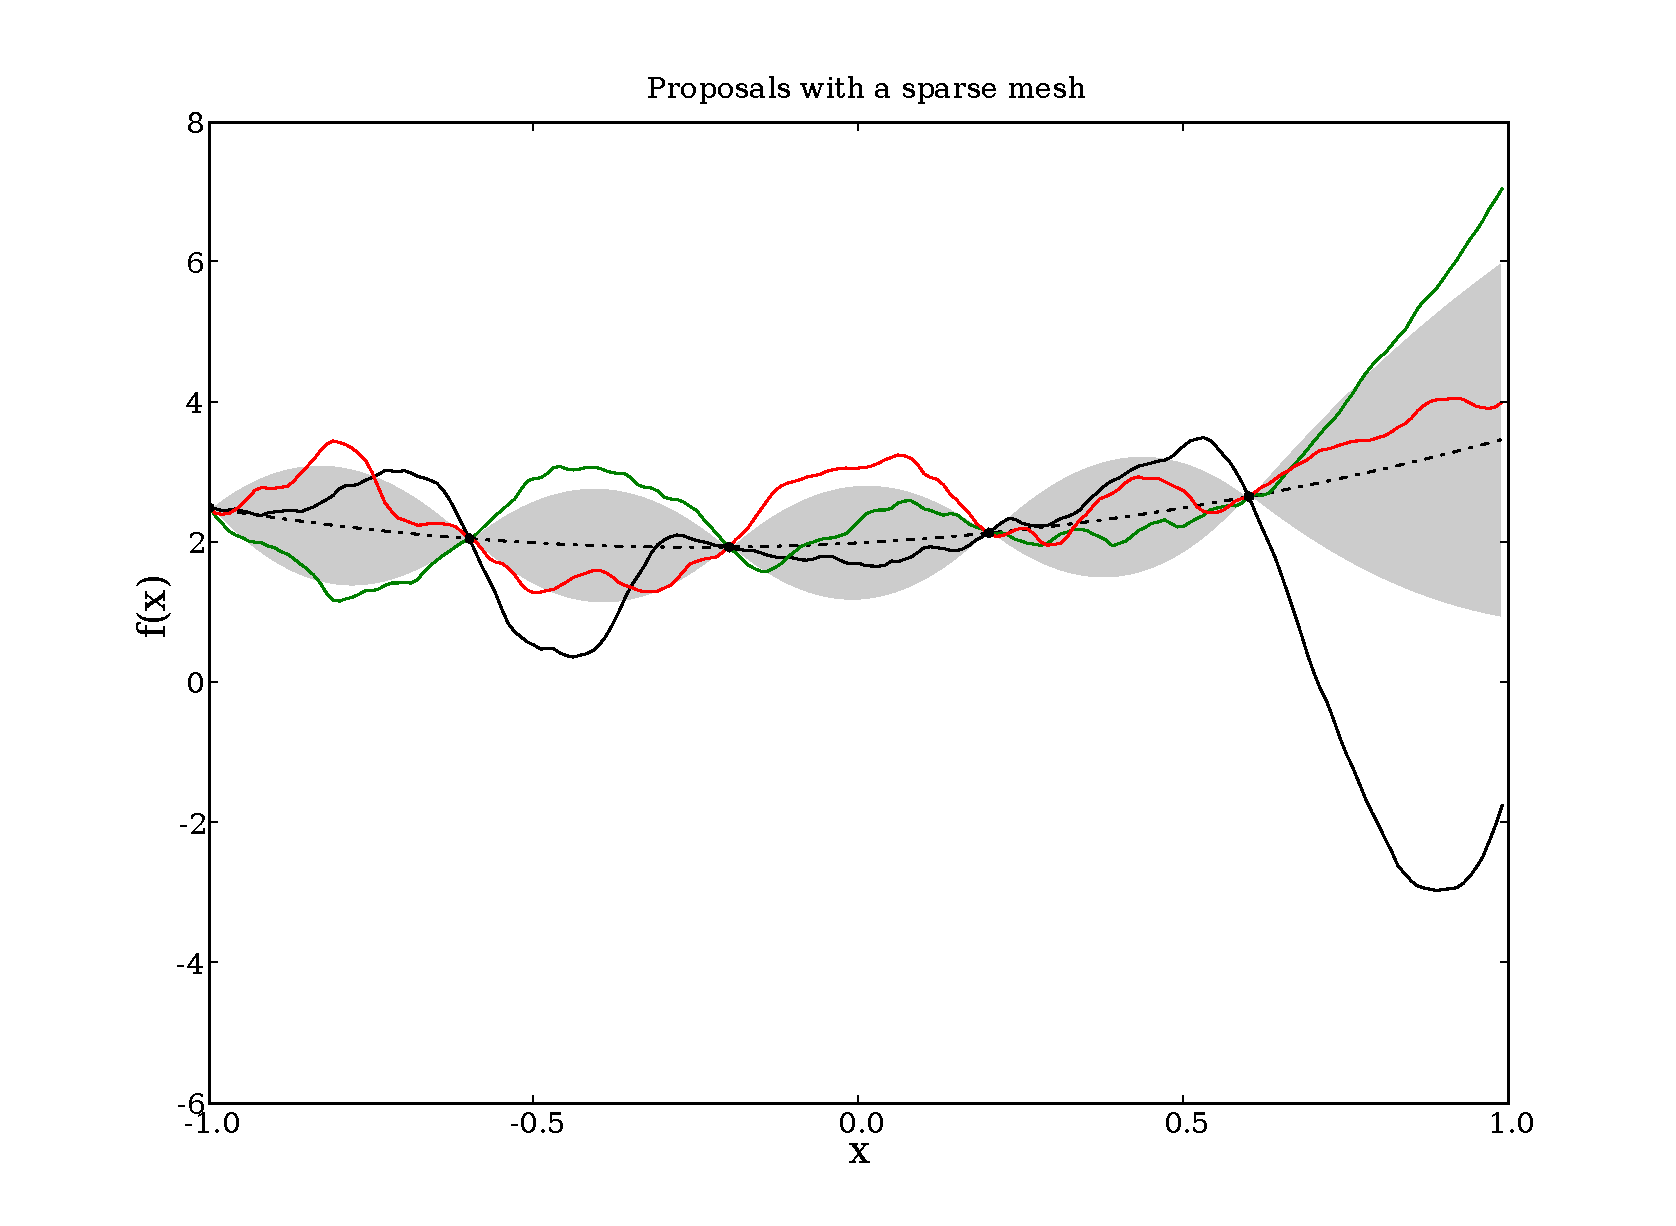
\epsfig{file=figs/lightmeshpropose.pdf,width=9cm}
        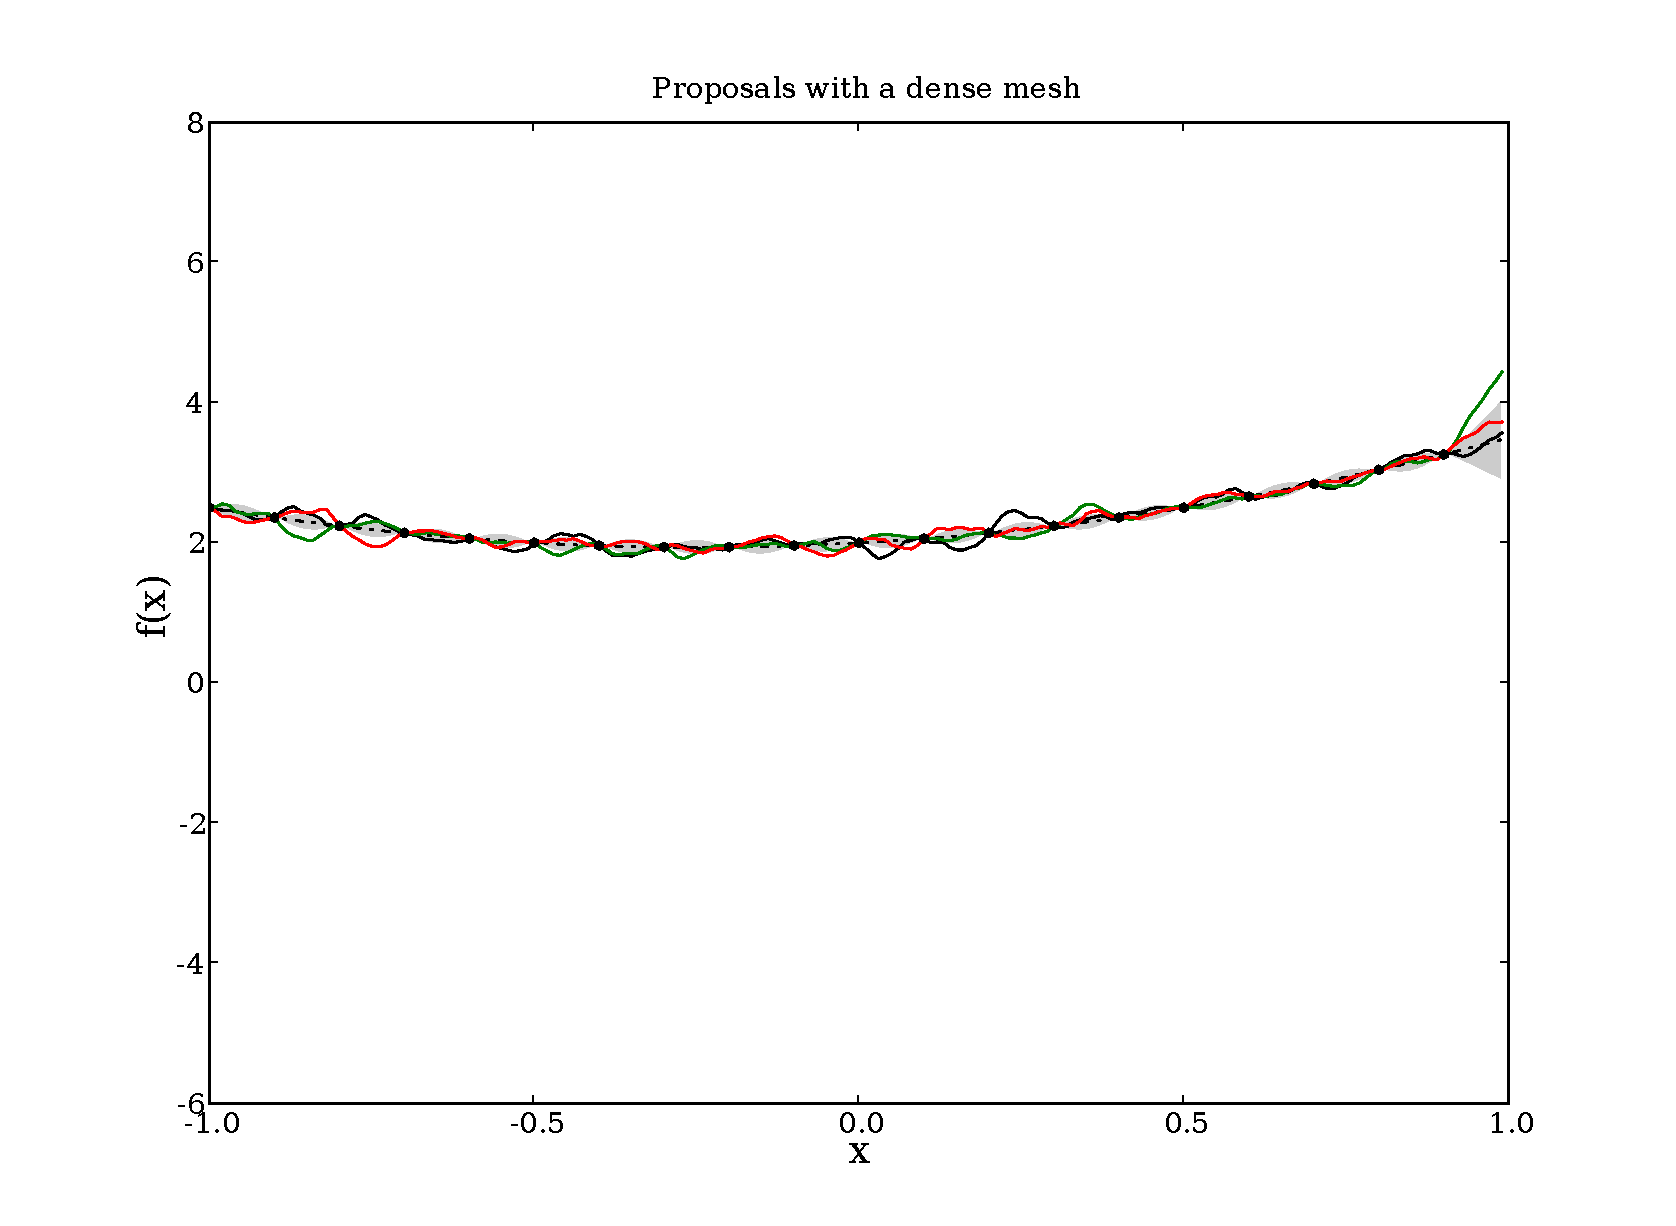
\epsfig{file=figs/densemeshpropose.pdf,width=9cm}
    \caption{Several possible proposals of $\tilde f$ (curves) given proposed values for $f(\texttt{mesh})$ (heavy dots) with no mesh (top), a sparse mesh (middle), and a dense mesh (bottom). Proposal distributions' envelopes are shown as shaded regions, with means shown as broken lines. With no mesh, $\tilde f$ is being proposed from its prior and the acceptance rate will be very low. A denser mesh permits a high degree of control over $\tilde f$, but computing the log-probability will be more expensive.}
    \label{fig:meshpropose}
\end{figure}


\section{The \class{GPNormal} step method}
As we've already seen in other contexts, a \class{GP}'s full conditional distribution is a Gaussian process if its Markov blanket is described by the following probability model:
\begin{eqnarray*}
    K_i |f \sim \textup{N}(f(o_i), V_i) & i=0\ldots n-1\\
    f|M,C\sim\textup{GP}(M,C)
\end{eqnarray*}
In other words, each of its children $K_i$ is normally distributed with variance $V_i$ and mean equal to $f(o_i)$, where $o_i$ is an arbitrary mesh.

In this case, a \texttt{GP} instance $f$ can be handled by the Gibbs step method \class{GPNormal}, which will have much better mixing properties that \class{GPMetropolis}. Its init method takes the following parameters:
\begin{description}
    \item[$f$:] The \texttt{GP} instance to be handled.
    \item[\texttt{obs_mesh:}] An array or array-valued variable giving the observation mesh $o$.
    \item[\texttt{obs_V}:] An array or array-valued variable giving the observation variance $V$.
    \item[\texttt{obs_vals}:] An array or array-valued variable giving the concatenation of the values of the children $K_i$.
\end{description}

\class{GPNormal} doesn't register itself, so it will never be assigned as a default handler. This may change eventually.

\class{GPNormal} doesn't care about $f$'s mesh, because it never has to evaluate $f$'s log-probability. However, a good choice of mesh is important because it will used by the \class{GPParentMetropolis} instances that handle $f$'s mean and covariance parameters.


% \section{Example: Ellner, Seifu and Smith's blowfly study}\label{sub:ESSMCMC}
%
% \textbf{I haven't been able to get this one to mix yet.} The model is:
% \begin{eqnarray*}
%     \textup{data}_t \stackrel{\tiny{\textup{ind}}}{\sim}(A_t, V)\\
%     A_t = B(A_{t-\tau})\psi_{t-\tau} - D(A_{t-1})\phi_{t-1}, & t>\tau\\
%     B \sim \textup{GP}(sx\exp(-rx), C_B) \\
%     D \sim \textup{GP}(mx, C_D) \\
%     \psi_t \stackrel{\tiny{\textup{iid}}}{\sim}\textup{lognorm}(\mu_\phi,V_\phi) \\
%     \phi_t \stackrel{\tiny{\textup{iid}}}{\sim}\textup{lognorm}(\mu_\phi,V_\phi)\\
%     C_B = \textup{Mat\`ern}(\sigma_B,\nu_B,\phi_B) \\
%     C_D = \textup{Mat\`ern}(\sigma_D,\nu_D,\phi_D)   \\
%     A_{1\ldots\tau},r,s,m,\textup{covariance parameters},\mu_\phi,\mu_\psi,V_\phi,V_\psi,V \sim \textup{priors},
% \end{eqnarray*}
% and I assumed $\tau$ fixed for purposes of the demo. The DAG schematic is shown in figure \ref{fig:ESSblowflymodel}.
%
% What happens is the following: when $B$ and $D$ have mean zero, the model burns in and mixes badly. When they have the mean functions parametrized above, the amplitude of their covariance params get very small; the model is preferring the simpler parametric version, since it can explain the data as well as the nonparametric version. This would make a great demo for both the importance of a flexible mean function and the natural parsimony of Bayesian statistics, but I can't even get the parametric version mixing and don't have time for week-long runs. We'll see what happens with this.
%
% \begin{figure}
%     \centering
%         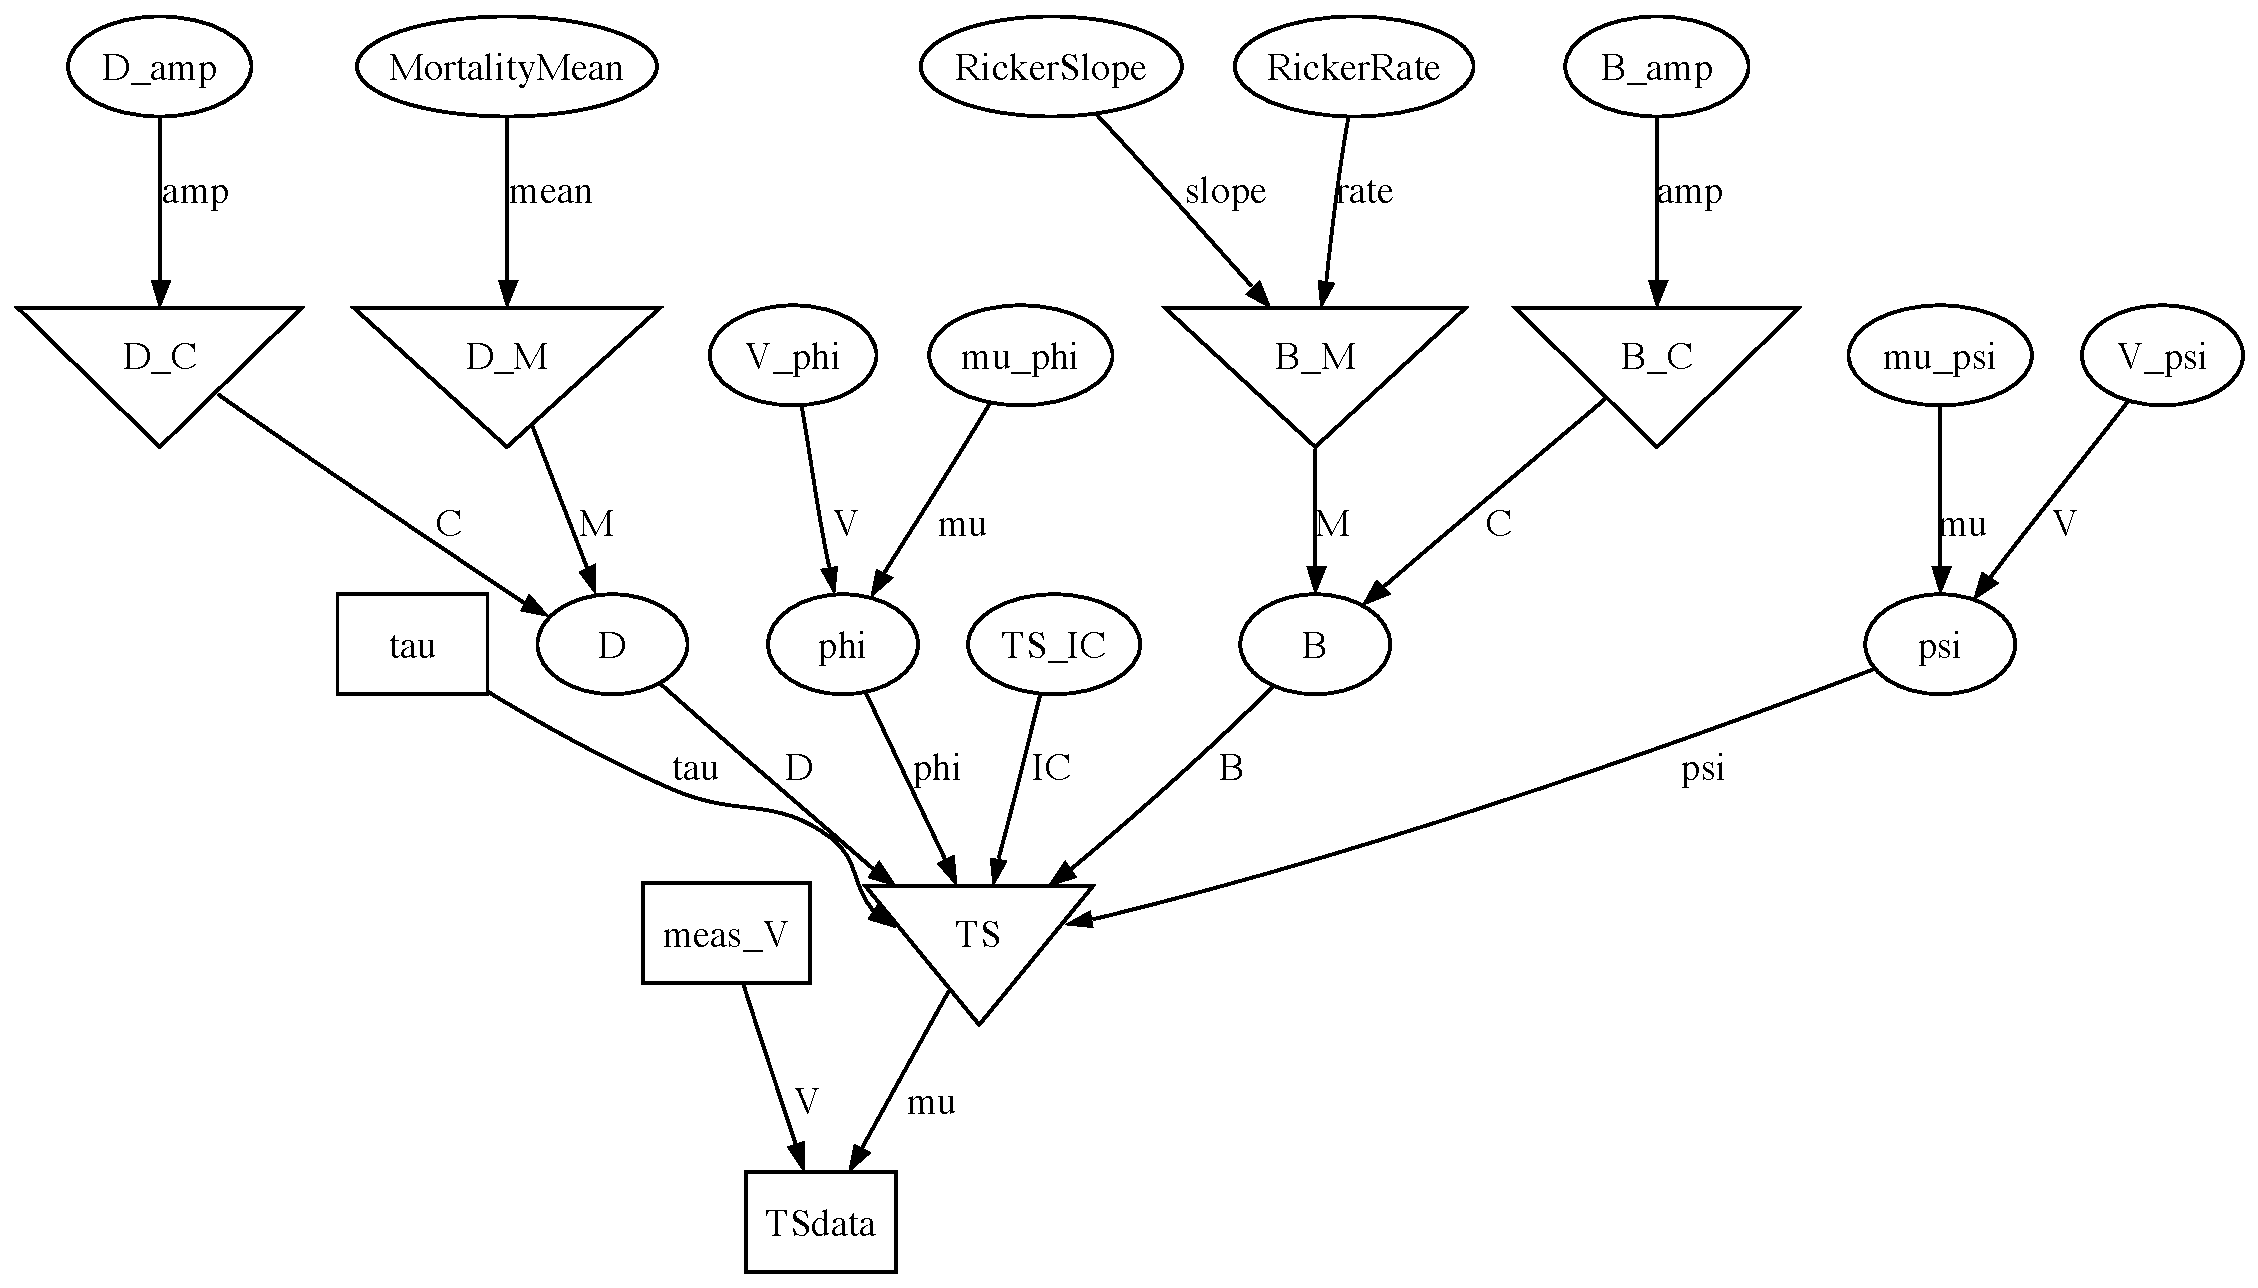
\epsfig{file=figs/ESSblowfly.pdf,width=15cm}
%     \caption{The model for Ellner, Seifu and Smith's \cite{ess} blowfly data.}
%     \label{fig:ESSblowflymodel}
% \end{figure}
%
% % \begin{figure}
% %     \centering
% %         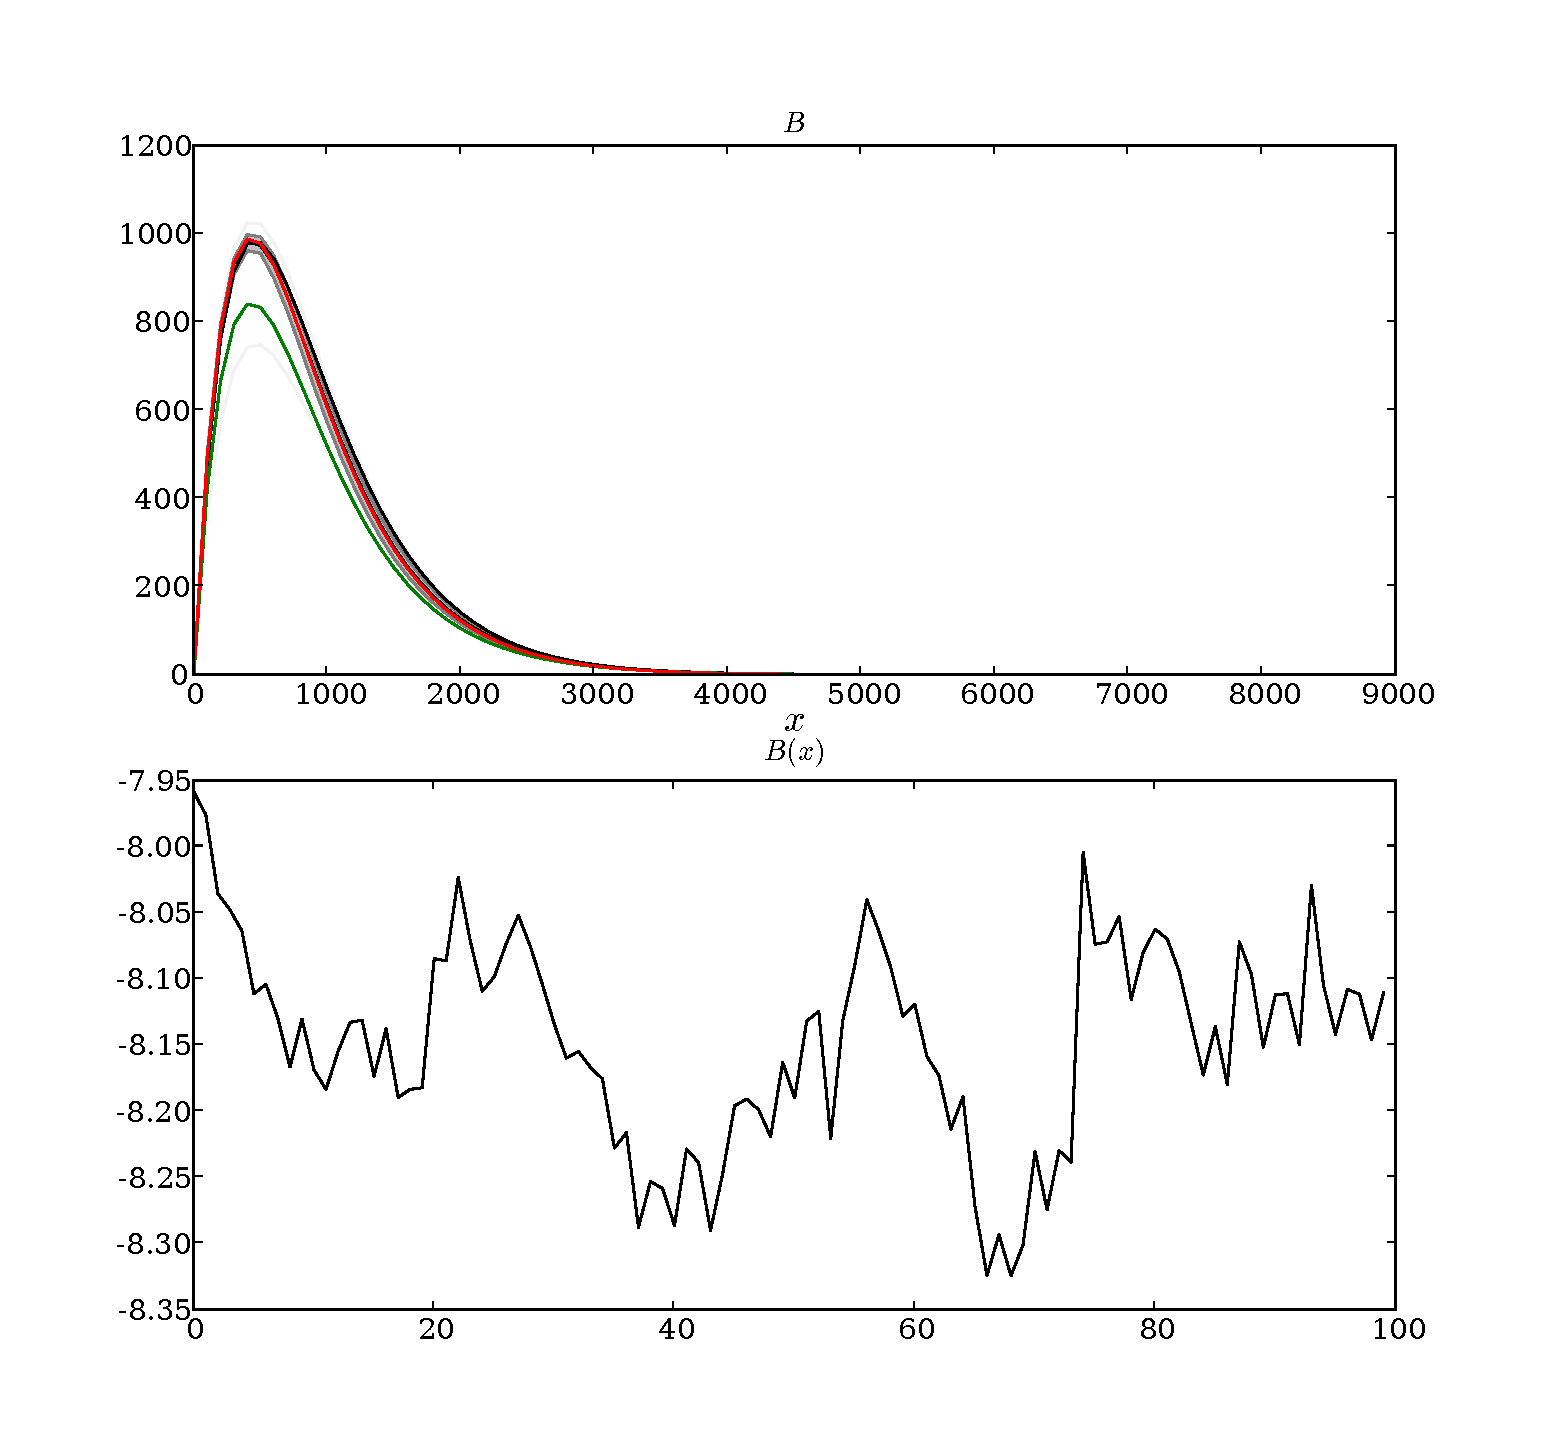
\epsfig{file=figs/ESSBPosterior.pdf,width=10cm}
% %         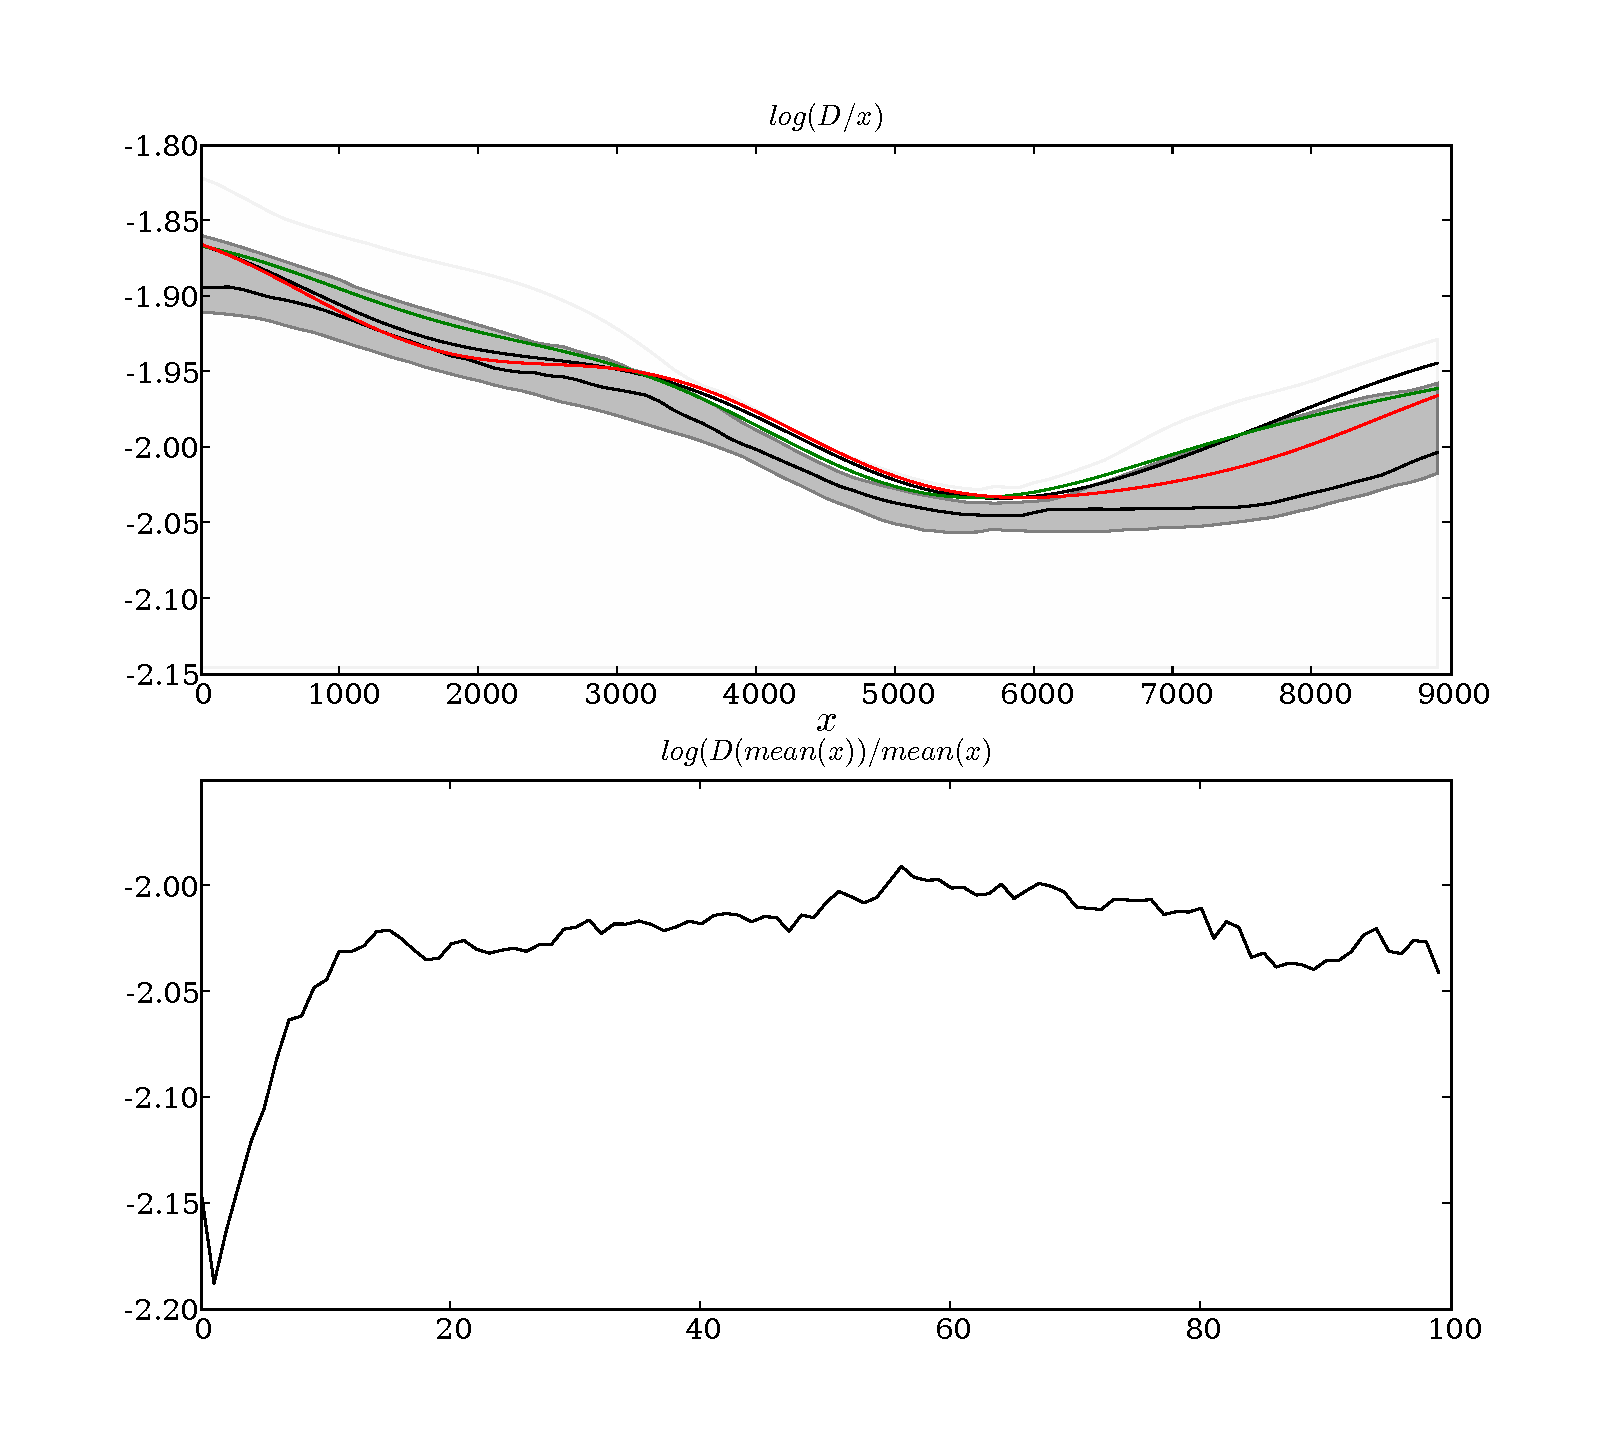
\epsfig{file=figs/ESSDPosterior.pdf,width=10cm}
% %     \caption{caption}
% %     \label{fig:ESSBD}
% % \end{figure}
% %
% % \begin{figure}
% %     \centering
% %         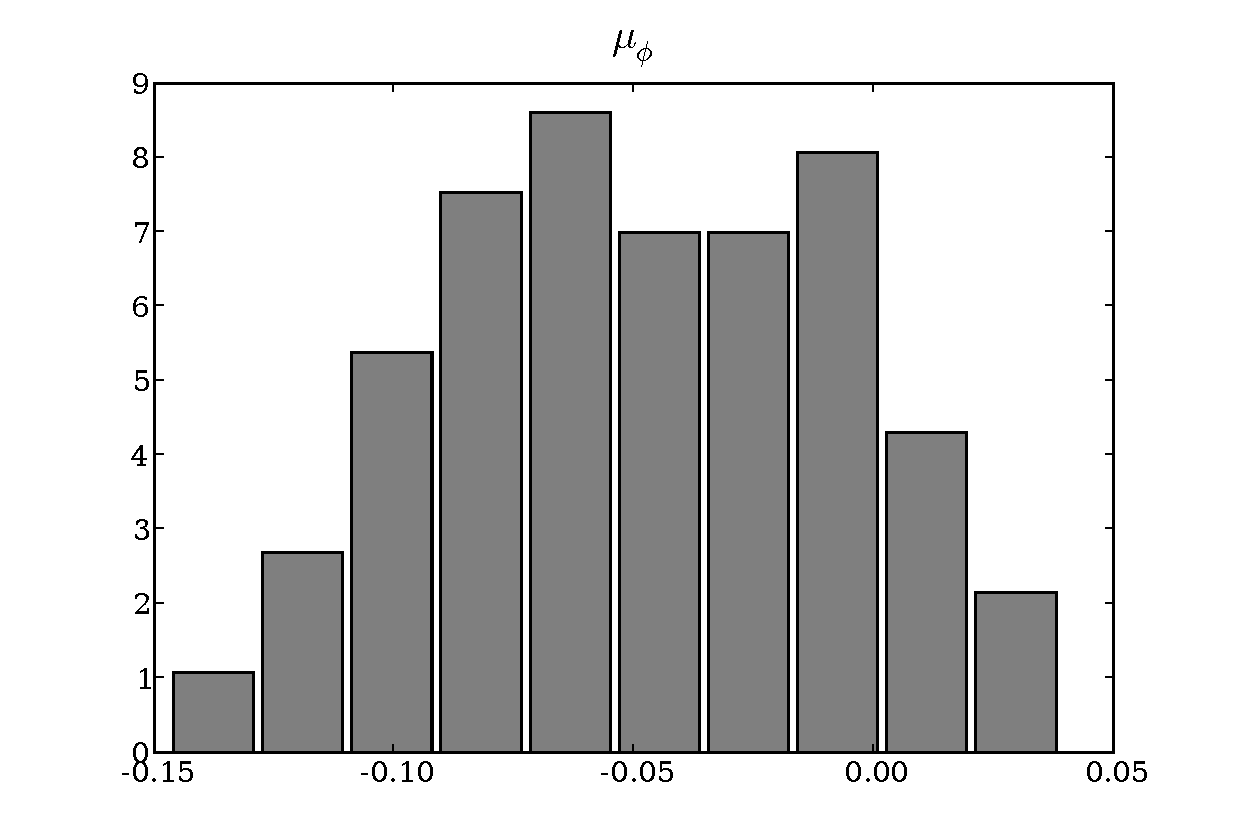
\epsfig{file=figs/ESSmuphiPosterior.pdf,width=7cm}
% %         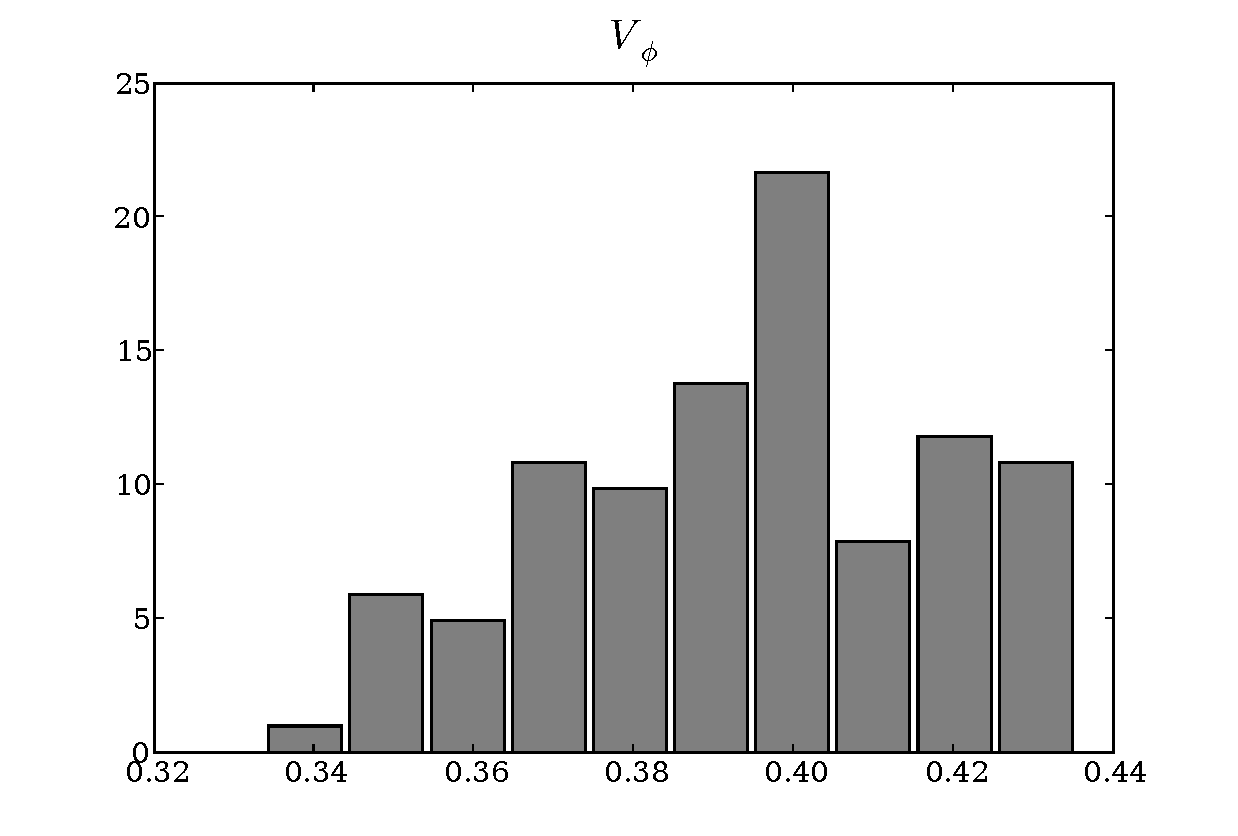
\epsfig{file=figs/ESSVphiPosterior.pdf,width=7cm}
% %         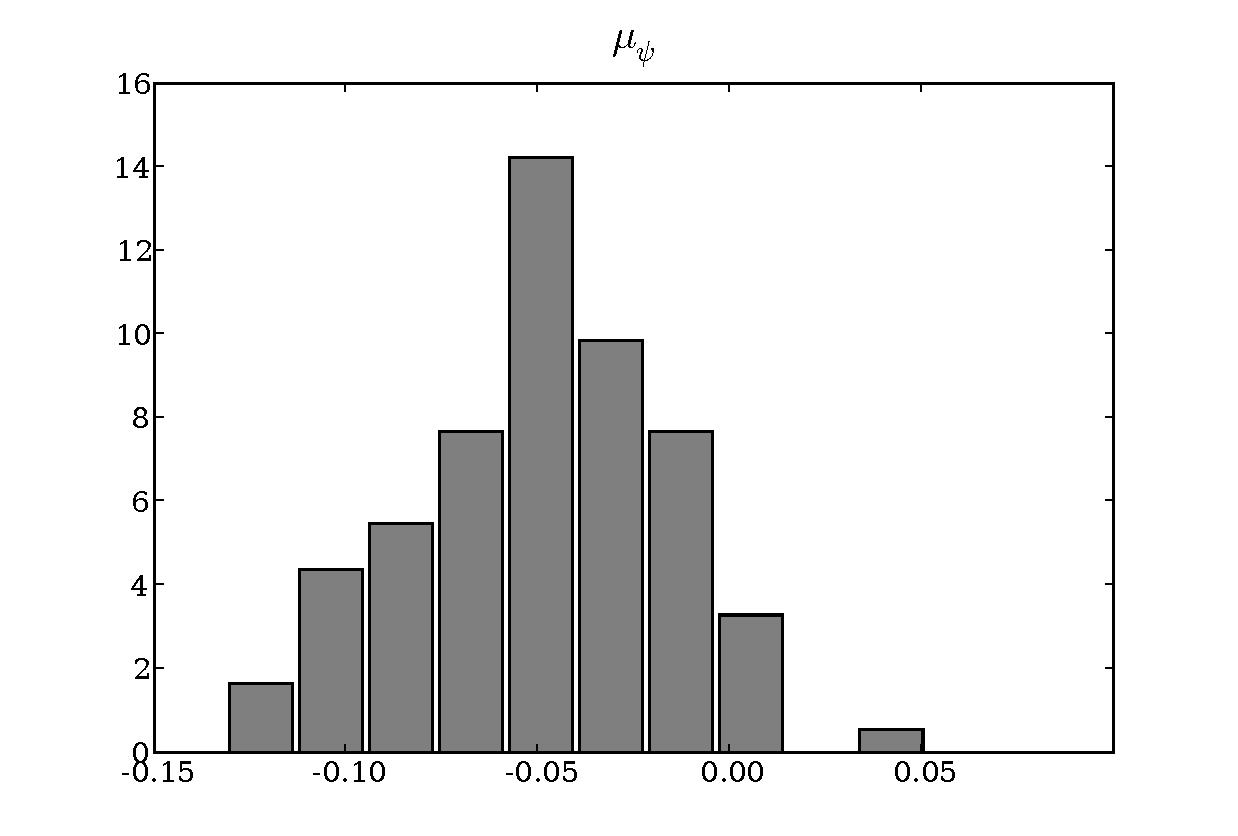
\epsfig{file=figs/ESSmupsiPosterior.pdf,width=7cm}
% %         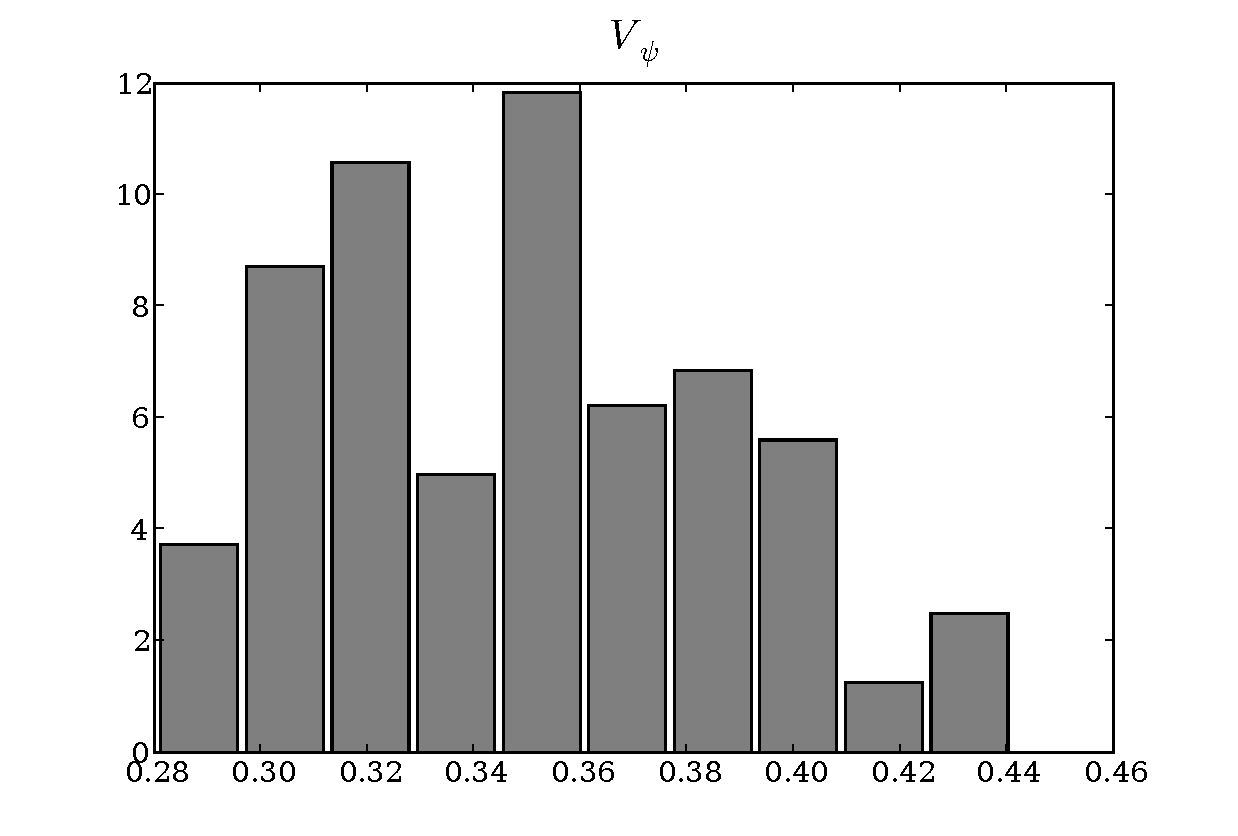
\epsfig{file=figs/ESSVpsiPosterior.pdf,width=7cm}
% %     \caption{caption}
% %     \label{fig:ESSphipsi}
% % \end{figure}
% %
% % \begin{figure}
% %     \centering
% %         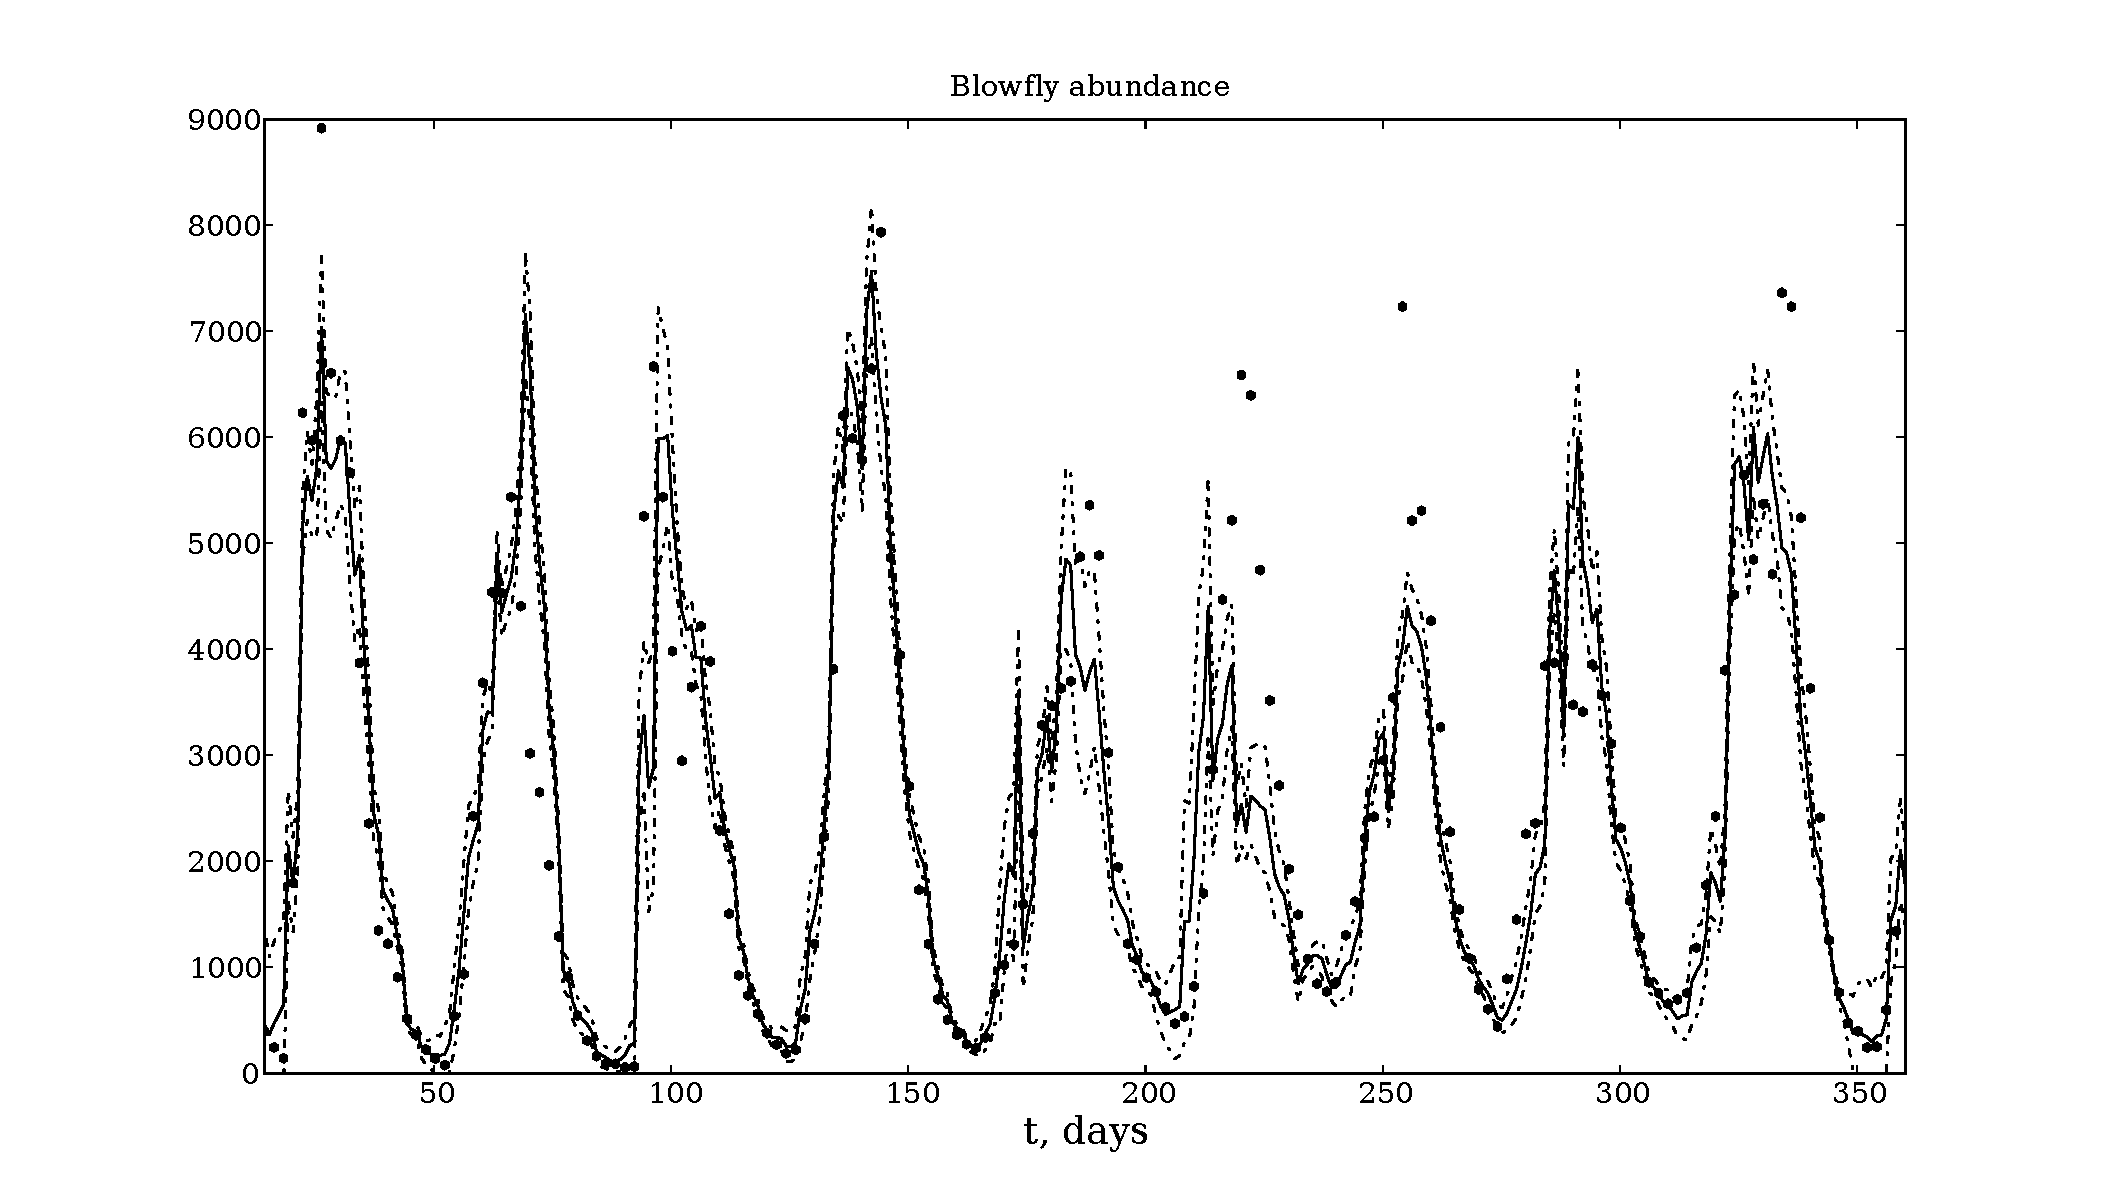
\epsfig{file=figs/ESSblowflyfit.pdf,width=15cm}
% %     \caption{caption}
% %     \label{fig:ESSfit}
% % \end{figure}
%
 

\chapter{Extending the covariance functions: Writing your own, using alternate coordinate systems, building in anisotropy and nonstationarity}\label{cha:usercov}
This section will give you a brief tour of the \module{cov_funs} module and point out plugs where you can add functionality that isn't included in this package.
\bigskip
Note that you don't need to understand this section; any covariance function that satisfies the calling convention described in section \ref{subsub:cov} will work. The \texttt{cov_funs} module is convenient, but it is admittedly complicated.

\bigskip
The \class{covariance_function_bundle} class includes versions of each covariance function using several different distance metrics. For example, the Euclidean version of the Mat\`ern covariance function is \texttt{matern.euclidean} and the Gaussian covariance function in geographic coordinates (in radians) is \texttt{gaussian.geo_rad}.

In addition, it has two attributes that are included for extensibility: the \texttt{raw} attribute, which exposes the basic Fortran implementation of each function, and \texttt{add_distance_metric} method, which combines the \texttt{raw} attribute with distance metrics. This section will describe these attributes in more detail.

Class \texttt{covariance_function_bundle}'s init method takes three arguments:
\begin{description}
	\item[\texttt{cov_fun_name}] The name of the covariance function.
	\item[\texttt{cov_fun_module}] The name of the module in which the covariance function can be found. This must be somewhere on your \texttt{PYTHONPATH}.
	\item[\texttt{extra_cov_params}] A dictionary whose keys are the extra parameters the covariance function takes, and whose values are brief sentences explaining the roles of those parameters. This dictionary will be used to generate the docstring of the bundle.
\end{description}
The names of the function and module are used rather than the function object itself in order to allow covariance objects to be pickled. This, in turn, allows covariance-valued stochastic variables to be stored in PyMC's \texttt{pickle} and \texttt{hdf52} database backends.


\section{The components of a covariance function bundle}

\section{The actual covariance functions}\label{sub:distances}
The covariance functions contained in a bundle are named by the distance metric they use. The \texttt{matern} bundle, for instance, contains the following covariance functions:
\begin{itemize}
	\item \texttt{matern.euclidean}
	\item \texttt{matern.geo_rad}
	\item \texttt{matern.geo_deg}
	\item \texttt{matern.aniso_geo_rad}
	\item \texttt{matern.aniso_geo_deg}
	\item \texttt{matern.paniso_geo_rad}
	\item \texttt{matern.paniso_geo_deg}
\end{itemize}

Each covariance function takes at least two arguments, $x$ and $y$, which are two-dimensional arrays in which the first index iterates over separate points and the second iterates over coordinates as in section \ref{sub:geostat}. For the geographic distance functions, the first coordinate is longitude and the second is latitude. Covariance functions also take arguments \texttt{amp} and \texttt{scale}. Finally, they take optional argument \texttt{symm}, which indicates whether $x$ and $y$ the same array.

Some of the covariance functions take extra arguments for the distance metric and/or actual covariance function. For example, \texttt{matern.aniso_geo_rad} takes extra arguments \texttt{inc} and \texttt{ecc} for the distance function and \texttt{diff_degree} for the covariance function.

When \texttt{matern.euclidean}, for example, is called with input locations $x$ and $y$, the following events place:
\begin{itemize}
	\item The output matrix is allocated.
	\item The output matrix is filled with the Euclidean distances between the elements of $x$ and the elements of $y$.
	\item The output matrix is overwritten with the covariances between the elements of $x$ and the elements of $y$.
\end{itemize}
The last two steps will be executed in parallel if environment variable \texttt{OMP_NUM_THREADS} is greater than 1 and the size of the output matrix is sufficiently large.

The easiest way to deal with different coordinate systems or to build in anisotropy and nonstationarity using a deformation approach \cite{sampson} is to write your own distance function and add it to the covariance function by calling the \texttt{add_distance_metric} method. See \ref{sub:add_distance_metric} for information on how to use your distance function with an existing covariance function, or with one of your own devising. See \ref{sub:user_ccs} for the calling conventions required from distance functions.

\section{The \member{raw} attribute}\label{sub:raw}
The \member{raw} attribute of each bundle is the underlying covariance function. These functions take distance matrices as arguments and overwrite them in-place as covariance matrices. If you write your own raw covariance function, it should conform to the standard described in section \ref{sub:user_ccs}.

The following raw functions are implemented in Fortran in \file{isotropic_cov_funs.f} and wrapped as covariance function bundles in \module{cov_funs}. Here $t$ denotes a single element of a distance matrix, $|x_i-y_j|$. Each function is equal to $1$ when $t=0$.
\begin{description}
    \item[\texttt{matern($\nu,t$)}:] The argument \texttt{diff_degree} is written in the following formula as $\nu$ for readability. $K_\nu$ is a modified Bessel function of the third kind of order $\nu$.
    \begin{eqnarray*}
        \frac{(2\sqrt{\nu}t)^\nu}{2^{\nu-1}\Gamma(\nu)}K_\nu(2\sqrt{\nu}t)
    \end{eqnarray*}
    \item[\texttt{quadratic($\texttt{phi},t$)}:]
    \begin{eqnarray*}
        1-\frac{t^2}{1+\phi t^2}
    \end{eqnarray*}
    \item[\texttt{gaussian($t$)}:]
    \begin{eqnarray*}
        e^{-t^2}
    \end{eqnarray*}
    \item[\texttt{pow_exp(\texttt{pow},$t$)}:] The argument \texttt{pow} is written as $p$.
    \begin{eqnarray*}
        e^{-|t|^p}
    \end{eqnarray*}
    \item[\texttt{sphere(t)}:]
    \begin{eqnarray}
        \left\{
        \begin{array}{ll}
            1-\frac{3}{2}t+\frac{1}{2}t^3& t\le 1\\
            0 & t > 1
        \end{array} \right.
    \end{eqnarray}
\end{description}

See \citetitle[http://www.statsnetbase.com/ejournals/books/book_summary/summary.asp?id=1285]{Banerjee et al.} \cite{banerjee} , \citetitle[http://www.leg.ufpr.br/mbgbook/]{Diggle and Ribeiro} \cite{diggle} and \citetitle[http://books.google.com/books?id=5n_XuL2Wx1EC&dq=stein+some+theory+for+kriging&printsec=frontcover&source=web&ots=829kgTWuC6&sig=gFu5_Gg4_eZ4yzFT4BBWamSanBA#PPP1,M1]{Stein} \cite{stein}for more discussion of the properties of these covariance functions. The init method of \texttt{covariance_function_bundle} takes just one argument, a raw covariance function.

\section{The \texttt{add_distance_metric} method and the \texttt{apply_distance} function}\label{sub:add_distance_metric}
\texttt{apply_distance} takes two arguments, a distance function and a raw covariance function, and returns a covariance function suitable for wrapping in a \class{Covariance} object.

It endows the new function with a docstring that combines the raw covariance function's information with the distance function's information. It's possible to include information about extra parameters in the auto-generated docstring. To wrap a raw covariance function with a distance function called \texttt{my_dist_fun} with extra parameters called \texttt{eta} and \texttt{gamma} you could add explanations to \texttt{my_dist_fun} before calling \texttt{apply_distance}:
\begin{verbatim}
my_dist_fun.extra_params = {'eta': 'The eta parameter.',
                            'gamma': 'The gamma parameter.'}
\end{verbatim}
The new parameters will be included in the docstring.

Covariance functions generated by \texttt{apply_distance} take the following arguments:
\begin{itemize}
    \item Input arrays $x$ and $y$. These high-level covariance functions are more forgiving than the distance functions; $x$ and $y$ do not actually need to be two-dimensional, the only requirement is that their last index must iterate over coordinates as in section \ref{sub:geostat}. The exception to this rule is if $x$ and $y$ are only one dimensional, in which case they are assumed to have only one coordinate.
    \item Scaling arguments \texttt{amp} and \texttt{scale}. Parameter \texttt{amp} is the standard deviation of $f(x)$ for arbitrary $x$, regardless of coordinate system, before observation (the prior standard deviation). Parameter \texttt{scale} controls the lengthscale of decay of the correlation, which controls the wiggliness of $f$. It effectively multiplies distances, so that large values yield quick decay and more wiggliness. These scaling arguments are sometimes referred to as the `sill' and `range' parameters.
    \item Extra arguments for the covariance and/or distance functions.
\end{itemize}

The \texttt{add_distance_metric} method of \class{covariance_function_bundle} is just a thin wrapper for the function \texttt{apply_distance}, which is in \file{cov_utils.py}. Since \class{covariance_function_bundle} objects already have a raw covariance function, this method only needs a distance function.



\section{Calling conventions for new covariance and distance functions}
\label{sub:user_ccs}

User-defined covariance and distance functions should always take the following arguments:
\begin{description}
	\item[$C$] A Fortran-contiguous (column major) array of dimension (\texttt{x.shape[0]},\texttt{y.shape[0]}). This should be overwritten in-place.
	\item[$x$, $y$] Arrays of input locations. These will be regularized: they will be two-dimensional, with the first index iterating over points and the second over coordinates.
	\item[\texttt{cmin}$=0$, \texttt{cmax}$=-1$] Optional arguments. If non-default values are provided, only the slice \texttt{C[:,cmin:cmax]} of $C$ should be overwritten.
	\item[\texttt{symm=False}] An optional argument indicating whether $x$ and $y$ are the same array. If \texttt{True}, $C$ will be square and only the upper triangle of $C$ should be overwritten.
\end{description}
They can take any other arguments they need, of course.

If parallel computation is desired, covariance and distance functions must release the \citetitle[http://www.python.org/doc/1.5.2/api/threads.html]{global interpreter lock}. That means they have to be written in Fortran or C. \citetitle[http://cens.ioc.ee/projects/f2py2e/]{f2py} extensions can release the global interpreter lock by simply including the statement \texttt{cf2py threadsafe}; other types of extensions should call the Python C-API macros \texttt{Py_BEGIN_ALLOW_THREADS} and \texttt{Py_END_ALLOW_THREADS}.

The high-level covariance functions produced by \texttt{apply_distance} will be more forgiving than these low-level distance and covariance functions; $x$ and $y$ will not actually need to be two-dimensional, the only requirement is that their last index must iterate over coordinates as in section \ref{sub:geostat}. The exception to this rule is if $x$ and $y$ are only one dimensional, in which case they are assumed to have only one coordinate. These high-level functions will regularize $x$ and $y$ before passing them into your distance and covariance functions.

User-supplied covariance functions should be expressed in their simplest forms: their amplitude and input scalings (`sill' and `range', when applicable) should be set to 1. No `nugget' parameter should be used. Numerically singular covariances are helpful when using \texttt{Covariance} objects, because they have low-rank Cholesky factors that can be used for efficient computation. The effect of a nugget can be obtained by adding iid normal variables to realizations. \texttt{FullRankCovariance} objects take a nugget argument regardless of their underlying covariance functions.

Distance functions should be symmetric, meaning the distance from point $x$ to point $y$ is the same as the distance from $y$ to $x$. Since raw covariance functions overwrite distance matrices, the output of an \texttt{apply_distance}-generated covariance function will be symmetric if its distance function is symmetric.

To be a valid covariance function, an \texttt{apply_distance}-generated covariance function $C$ must be positive semidefinite, meaning $C(x,x)$ is a positive semidefinite matrix for any mesh $x$. The formal test for positive semidefiniteness is Bochner's theorem \cite{stein}.%, but you can also just check the eigenvalues of $C(x,x)$ for a variety of meshes $x$.



\section{Summary}\label{sec:cookbook}
\begin{description}
    \item[To use a new functional form:] Write a new raw covariance function and wrap it in a \class{covariance_function_bundle} object.
    \item[To use a new coordinate system:] Write a new distance function and use the \texttt{add_distance_metric} method of an existing \class{covariance_function_bundle}.
    \item[To build in anisotropy/ nonstationarity using a deformation approach] like that of Sampson and Guttorp \cite{sampson}, you can either write a new distance function and use \texttt{add_distance_metric} or you can actually implement the deformation before passing in the $x$ and $y$ arguments, possibly using PyMC \class{Deterministics}.
    \item[To use a new functional form \emph{and} a new distance function:] Wrap the covariance function as a \class{covariance_function_bundle} and apply the \texttt{add_distance_metric} method to the distance function, or just apply \texttt{apply_distance} to both of them at once.
\end{description}

The easiest way to implement a more advanced extension like that of Paciorek and Schervish \cite{pachische} , is to write a new wrapper like \texttt{apply_distance}. You'll probably still be able to take advantage of the raw covariance functions, but not the distance functions. If you do this and don't mind sharing your work, please email me.



\chapter{Overview of algorithms} \label{cha:numerics} 
More detail on these algorithms, as well as the internal workings of the mean, covariance and realization objects and the observe function, are given in the algorithm documentation. 
\section{Gaussian processes and the multivariate normal distribution}

Gaussian processes generalize the multivariate normal distribution from vectors to functions, like the multivariate normal distribution generalizes the univariate normal distribution from scalars to vectors. The progression is as follows:
\begin{equation}
    \begin{array}{ll}
        y\sim\textup N(\mu,V): & \textup{$y$, $\mu$, $V$ are scalars}\\\\
        \vec y\sim\textup N(\vec \mu,C): & \textup{$\vec y$ and $\vec \mu$ are vectors, $C$ is a matrix}\\\\
        f\sim\textup{GP}(M, C): & \textup{$f$ and $M$ are functions of one variable, $C$ is a function of two variables}
    \end{array}
\end{equation}

One of the nice things about all Gaussian distributions (parameterized by mean and covariance) is that they're easy to marginalize. For example, each element of a vector with a multivariate normal distribution has a univariate normal distribution:
\begin{eqnarray*}
    \vec y\sim\textup N(\vec \mu,C)\\
    \Rightarrow \vec y_i\sim\textup N(\vec \mu_i,C_{i,i}),
\end{eqnarray*}
and any subvector of a vector with a multivariate normal distribution has a multivariate normal distribution:
\begin{eqnarray*}
    \vec y\sim\textup N(\vec \mu,C)\\
    \Rightarrow \vec y_{i_1\ldots i_2}\sim\textup N(\vec \mu_{i_1\ldots i_2},C_{i_1\ldots i_2,i_1\ldots i_2}).
\end{eqnarray*}

This marginalizability applies to GP's as well. If $\vec x$ is a vector of values,
\begin{equation}
    \begin{array}{l}
        f\sim\textup{GP}(M, C)\\\\
        \Rightarrow f(\vec x) \sim\textup N(M(\vec x), C(\vec x,\vec x)).
    \end{array}
\end{equation}
In other words, any evaluation of a Gaussian process realization has a multivariate normal distribution. Its mean is the corresponding evaluation of the associated mean function, and its covariance is the corresponding evaluation of the associated covariance function. You can probably start to see why this fact is important for working with GPs on a computer.

\subsection{Observations}
As mentioned earlier, if $f$ has a GP prior and normally-distributed observations of $f$ are made at a finite set of values, $f$'s posterior is a Gaussian process also:
\begin{eqnarray*}
    \left.\begin{array}{l}
        d_i \stackrel{\tiny{\textup{ind}}}{\sim} \textup{N}(f(o_i), V_i)\\
        f \sim \textup{GP}(M,C)
    \end{array}\right\}\Rightarrow f|d \sim \texttt{GP}(M_o, C_o).
\end{eqnarray*}
Denoting by $o$ the array of observation values $[o_0\ldots o_{N-1}]$ and $V$ a matrix with observation variances $[V_0\ldots V_{N-1}]$ on its diagonal, $M_o(x)$ and $C_o(x,y)$ are as follows for arbitrary input vectors $x$ and $y$:
\begin{eqnarray*}
    M_o(x) = M(x) + C(x,o)[C(o,o) + V]^{-1}(f(o)-M(o))\\
    C_o(x,y) = C(x,y) - C(x,o)[C(o,o) + V]^{-1}C(o,y).
\end{eqnarray*}

\subsection{Low-rank observations}

If $C(o,o)+V$ is singular, some elements of $f(o)$ can be computed from others with no uncertainty. In other words, there exists a partition $[o_*, o_{**}]$ of $o$ and corresponding partition of the data such that $C(o_*,o_*)+V$ is full-rank and
\begin{eqnarray*}
    f(o_{**}) = M_{o_*}(o_{**}),
\end{eqnarray*}
where $M_{o_*}$ can be computed from the formula above.

In such cases, this package's strategy is to observe $f$ at a subvector $o_*$ of $o$, such that $C(o_*,o_*)+V$ is full-rank but if any elements were added to $o_*$ it would pick up a very small eigenvalue. The function \function{predictive_check} optionally checks the remaining data values $d_{**}$ against $M_{o_*}(o_{**})$, and raises an error if the two aren't equal up to a user-defined threshold.

This threshold is parameter \code{relative_precision} from \texttt{Covariance}'s init method, multiplied by the largest value on the diagonal of $C(o_*,o_*)+V$; intuitively, the maximal variance of $f(o_{**})$ given $f(o_*)$ is a multiple of the maximal variance of $f(o_*)$.

\section{Incomplete Cholesky factorizations}\label{sec:ichol} % (fold)

In addition to numpy's linear algebra support, this package uses some Fortran subroutines wrapped using \citetitle[http://cens.ioc.ee/projects/f2py2e/]{f2py}. They require \citetitle[http://www.netlib.org/blas/]{BLAS} and \citetitle[http://www.netlib.org/lapack/]{LAPACK} libraries (eg, \citetitle[http://math-atlas.sourceforge.net/]{ATLAS}) on your system, and the \file{setup.py} script will attempt to find these. If you don't have optimized BLAS and LAPACK installed, it's a good idea to install them; this package and numpy in general will be much faster. Some operating systems (such as Mac OS X) ship with optimized BLAS and LAPACK libraries included.

The following incomplete Cholesky factorization functions are found in the Fortran files \file{linalg_utils.f} and \file{incomplete_chol.f} :
\begin{description}

    % \item[\function{dtrsm_wrap(a,b,uplo='U',transa='N',alpha=1.)}:] A wrapper for the BLAS routine \citetitle[http://www.netlib.org/blas/dtrsmf.f]{DTRSM}, which solves triangular systems \texttt{$\alpha$a$^{op}$ x = b} in-place (that is, \texttt{b} is overwritten by $x$).
    % \begin{itemize}
    %     \item If \texttt{uplo='U'}, \texttt{a} is assumed to be an upper triangle; if \texttt{uplo='L'}, \texttt{a} is assumed to be a lower triangle.
    %     \item If \texttt{transa='T'}, \texttt{$\alpha$a.T*x = b} is solved. If \texttt{transa='N'}, \texttt{$\alpha$a*x = b} is solved.
    % \end{itemize}
    % 
    % \item[\function{dtrmm_wrap(a,b,uplo='U',transa='N',alpha=1.)}:] A wrapper for the BLAS routine \citetitle[http://www.netlib.org/blas/dtrsmf.f]{DTRMM}, which does the triangular matrix multiplication \texttt{$\alpha$a$^{op}$x = b} in-place (that is, \texttt{b} is overwritten by $x$).
    % \begin{itemize}
    %     \item If \texttt{uplo='U'}, \texttt{a} is assumed to be an upper triangle; if \texttt{uplo='L'}, \texttt{a} is assumed to be a lower triangle.
    %     \item If \texttt{transa='T'}, \texttt{$\alpha$a.T*x} is computed. If \texttt{transa='N'}, \texttt{$\alpha$a*x} is computed.
    % \end{itemize}
    % 
    % \item[\function{info = dpotrf_wrap(a)}:] A wrapper for the LAPACK routine \citetitle[http://www.netlib.org/lapack/double/dpotrf.f]{DPOTRF}, which tries to overwrite positive-definite matrix \texttt{a} with an upper-triangular Cholesky factor in-place. If the return value \texttt{info} is positive, \texttt{a} is not positive definite and the algorithm has failed.

    \item[\function{U, m, piv = ichol(diag, reltol, rowfun)}:] An implementation of the incomplete Cholesky decomposition, based on a port of one of the functions in the \citetitle[http://www.kyb.tuebingen.mpg.de/bs/people/seeger/]{chol_incomplete} package by Matthias Seeger.

The arguments are:
    \begin{description}
        \item[\texttt{diag}:] The diagonal of an \texttt{n} by \texttt{n} covariance matrix C.
        \item[\texttt{reltol}:] If the ratio of the \texttt{i}'th pivot to the maximum pivot is found to be less than \texttt{reltol}, the \texttt{i}'th pivot is assumed to be zero.
        \item[\texttt{rowfun}:] A Python function. The call \function{rowfun(i,p,rowvec)} should perform the update \texttt{rowvec[i,i+1:]=C[i,p[i+1:]]} in-place.
    \end{description}

The outputs are:
    \begin{description}
        \item[M:] The rank of C. Note that M$\le$\texttt{n}.
        \item[\texttt{piv}:] A length-\texttt{n} vector of pivots.
        \item[\texttt{U}:] An M-by-\texttt{n} upper-triangular matrix that satisfies \texttt{U[:,argsort(piv)].T * U[:,argsort(piv)] = C}.
    \end{description}

Because the full matrix $C$ does not need to be computed ahead of time, the algorithm is able to factor $C$ in $O(m^2 n)$ operations \cite{incompchol}. The algorithm is implemented in Fortran, but a Python version would be as follows:

\begin{verbatim}

def swap(vec,i,j):
    temp = vec[i]
    vec[i] = vec[j]
    vec[j] = temp

def ichol(diag, reltol, rowfun):

    piv = arange(n)
    U = zeros((n,n),dtype=float).view(matrix)
    rowvec = zeros(n,dtype=float)

    for i in range(n):
        l = diag[i:].argmax()
        maxdiag = diag[l]

        if maxdiag < reltol:
            m=i
            return U[:m,:], m, piv

        swap(diag,i,l)
        swap(p,i,l)

        temp = U[:i,i]
        U[:i,i] = U[:i,l]
        U[:i,l] = temp


        U[i,i] = sqrt(diag[i])
        rowvec[i:] = C[i,piv[i+1:]]

        if i > 0:
            rowvec -= U[:i,i].T * U[:i,i+1:]

        U[i,i+1:] = rowvec[i+1:] / U[i,i]
        diag[i+1:] -= U[i,i+1:].view(ndarray) ** 2

    m=n
    return U, m, piv
\end{verbatim}

Function \function{ichol} is wrapped by the \class{Covariance} method \method{cholesky}.

\item[\function{m, piv = ichol_continue(U, diag, reltol, rowfun, piv)}:]
This function computes the Cholesky factorization of an \texttt{n} by \texttt{n} covariance matrix C from the factor of its upper-left \texttt{n}$_*$ by \texttt{n}$_*$ submatrix C$_*$. Its input arguments are as follows:
\begin{description}
    \item[\texttt{U}:] Unlike \function{ichol}, this function overwrites a matrix in-place. Suppose the Cholesky factor of C$_*$, \texttt{U}$_*$, is of rank M$_*$. On input, \texttt{U} must be an \texttt{[m + (n-n$_*$)]}-by-\texttt{n} matrix arranged like this:
    \begin{eqnarray*}
        \left[
        \begin{array}{ccc}
            \texttt{U}_*\texttt{[:,:m}_*\texttt{]} & \texttt{U}_*\texttt{[:,:m}_*\texttt{].T.I C[:m}_*\texttt{,n}_*\texttt{:]} & \texttt{U}_*\texttt{[:,m}_*\texttt{:]}\\
            \texttt{0}&\texttt{0}&\texttt{0}
        \end{array}
        \right]
    \end{eqnarray*}
On exit, \texttt{U} will be an M-by-\texttt{n} upper-triangular matrix that satisfies \texttt{U[:,argsort(piv)].T * U[:,argsort(piv)]=C}.
    \item[\texttt{piv}:] Denote by \texttt{piv}$_*$ the pivot vector associated with \texttt{U}$_*$ On input, \texttt{piv} must be a length-\texttt{n} vector laid out like this:
    \begin{eqnarray*}
        \begin{array}{ccc}
            [\texttt{piv}_*\texttt{[:m}_*\texttt{]} & \texttt{arange(n-n$_*$)} & \texttt{piv}_*\texttt{[m}_*\texttt{:]}]
        \end{array}
    \end{eqnarray*}
    \item[\texttt{diag}:] The length \texttt{n-n}$_*$ diagonal of \texttt{C[n$_*$:,n$_*$]}.
    \item[\texttt{rowfun}:] The call \function{rowfun(i,p,rowvec)} should perform the update \texttt{rowvec[i,i+1:]} \texttt{=} \texttt{C[i,p[i+1:]]} in-place.
\end{description}

    The input parameter \texttt{reltol}, as well as the output parameters \texttt{piv} and M and the updated matrix \texttt{U}, should be interpreted just like their counterparts in \function{ichol}.

    The algorithm is just like the algorithm in ichol, but the index \texttt{i} iterates over \texttt{range(m$_*$,m$_*$+n-n$_*$)} (and the index of \texttt{diag} is downshifted appropriately).

    \function{ichol_continue} is wrapped by the \class{Covariance} method \method{continue_cholesky}, so it should rarely be necessary to call it directly.

    \item[\function{U, m, piv = ichol_full(c, reltol)}:] Just like \texttt{ichol}, but instead of a diagonal and a `get-row' function a full covariance matrix C is required as an input.

    \item[\function{U, m, piv = ichol_full(basis, nug, reltol)}:] Just like \texttt{ichol}, but the following arguments are required:
    \begin{description}
        \item[\texttt{basis}:] The evaluation of a basis function on the mesh, multiplied by the Cholesky factor of the coefficients' covariance matrix. This is itself a square root of the covariance matrix, but running it through \texttt{ichol_basis} allows for observations with nonzero variance and essentially pivots for better accuracy even in the zero-variance case.
        \item[\texttt{nug}:] A vector that will effectively be added to the diagonal of the covariance matrix.
    \end{description}
\end{description}

%     \item[\function{x = trisolve(A,b,uplo='U',transa='N',inplace=False)}:] Solves the triangular system \texttt{$\alpha$a$^{op}$ x = b} using \function{dtrsm_wrap} and returns $x$. If \texttt{A} is found to be singular, an error is raised.
%     \begin{itemize}
%         \item \texttt{A} is assumed upper-triangular if \code{uplo='U'} and lower-triangular if \code{uplo='L'}.
%         \item If \texttt{transa='T'}, \texttt{$\alpha$a.T*x = b} is solved. If \texttt{transa='N'}, \texttt{$\alpha$a*x = b} is solved.
%         \item If \texttt{inplace=True}, \texttt{b} is overwritten with $x$ in-place and returned. If \texttt{inplace=False}, \texttt{b} is not modified.
%     \end{itemize}
% 
%     \item[\function{b = trimult(A,x,uplo='U',transa='N',inplace=False)}:] Does the triangular multiplication \texttt{$\alpha$a$^{op}$x = b} using \function{dtrmm_wrap} and returns \texttt{b}.
%     \begin{itemize}
%         \item \texttt{A} is assumed upper-triangular if \code{uplo='U'} and lower-triangular if \code{uplo='L'}.
%         \item If \texttt{transa='T'}, \texttt{$\alpha$a.T8x} is computed. If \texttt{transa='N'}, \texttt{$\alpha$a*x} is computed.
%         \item If \texttt{inplace=True}, $x$ is overwritten with \texttt{b} in-place and returned. If \texttt{inplace=False}, $x$ is not modified.
%     \end{itemize}
% \end{description}

    % \item[\function{observe(M, C, obs_mesh, obs_vals, obs_V, lintrans, cross_validate = True)}:] This function calls \texttt{C.observe}, calls \texttt{M.observe} with the output, and then if \texttt{cross_validate=True} calls \texttt{predictive_check}.

%     If the return of \texttt{predictive_check} value is \texttt{False}, the values of some observations can be predicted with negligible uncertainty from the values of others, but they don't match their predicted values; in other words, the data are extremely improbable. A \texttt{ZeroProbability} exception is raised with some helpful suggestions if this is the case.
%
%     \item[\function{OK = predictive_check(obs_vals, obs_mesh, M, posdef_indices, tolerance)} :] Checks the value of M evaluated at \texttt{obs_mesh} sliced at the complement of \texttt{posdef_indices} against the corresponding \texttt{obs_vals}. If any of the differences are greater than \texttt{tolerance}, \texttt{False} is returned. Otherwise \texttt{True} is returned.
% \end{description}
% \section{Object internals}\label{sec:internals}
%
% The methods of \class{Mean}, \class{Covariance} and \class{Realization} will be described here.
%
% \section{Covariance}\label{sec:covarianceInt}
% \begin{description}
%
%     \item[\method{cholesky(x, apply_pivot = True, observed=True)}:] Returns an incomplete Cholesky factor of \texttt{C(x,x)}. The other arguments' meanings are as follows:
%     \begin{description}
%         \item[\texttt{apply_pivot}:] If \texttt{True}, the return value is a matrix \texttt{U} such that \texttt{U.T*U = C(x,x)}. If \texttt{False}, the return value is a dictionary. Element \texttt{'pivots'} is a vector of pivots returned by function \function{ichol}, and element \texttt{'U'} is the matrix \texttt{sig} returned by \function{ichol}.
%         \item[\texttt{observed}:] If \texttt{True}, the matrix \texttt{C(x,x)} is obtained conditional on observations that have been made involving C. If \texttt{False}, the matrix is obtained without regard to those observations.
%     \end{description}
%
%         \item[\method{continue_cholesky(x, x_old, chol_dict_old[, apply_pivot, observed])}:] Returns an incomplete Cholesky factor of \texttt{C(concatenate(x_old,x), concatenate(x_old,x))}. Arguments \texttt{apply_pivot} and \texttt{observed} are the same as for \texttt{cholesky}. \texttt{chol_dict_old} should be the incomplete Cholesky factorization of \texttt{C(x_old, x_old)} in the form of a dictionary such as the one produced by \texttt{C.cholesky}.
%
%         This method returns either a matrix or a dictionary depending on the value of \texttt{apply_pivot}. See \texttt{cholesky}.
%
%
%         \item[\method{relevant_slice, obs_mesh_new, U_for_draw = observe(obs_mesh, obs_V=0.)}:] All subsequent calls will be made under the assumption that observations of the random field at inputs \texttt{obs_mesh} have been made with variance \texttt{obs_V}. This method updates the following attributes of C:
%         \begin{itemize}
%             \item \texttt{observed}: This flag is set to \texttt{True}.
%             \item \texttt{obs_U} and \texttt{obs_piv}: The output of \texttt{self.cholesky(obs_mesh, apply_pivot=False, observed=False)}.
%             \item \texttt{obs_mesh}: The mesh on which self has been observed, sliced by \texttt{obs_piv[:m]}, where M is the rank of \texttt{obs_U}.
%             \item \texttt{obs_V}: The variances associated with the observations, sliced as \texttt{obs_mesh} is.
%             \item \texttt{obs_len}: The length of \texttt{obs_V}.
%         \end{itemize}
%
%         The return values are:
%         \begin{itemize}
%             \item \texttt{relevant_slice}: The indices included in the incomplete Cholesky factorization. These correspond to the values of \texttt{obs_mesh} that determine the other values, but not one another.
%             \item \texttt{obs_mesh_new}: \texttt{obs_mesh} sliced according to \texttt{relevant_slice}.
%             \item \texttt{U_for_draw}: An upper-triangular Cholesky factor of \texttt{self}'s evaluation on \texttt{obs_mesh} conditional on all previous observations.
%         \end{itemize}
%
%
%
%     \item[\method{__call__(x[, y, observed])}:]
%
%     \begin{itemize}
%         \item If only one argument $x$ is provided, \texttt{C(x,x) = V(f(x))} will be returned conditional on any observations that have been made.
%         \begin{itemize}
%             \item If C is unobserved or \texttt{observed = False}, its underlying function C is evaluated at each element of $x$. The \texttt{i}'th element of the return value is \texttt{c(x_i,x_i)}.
%             \item If C is observed and \texttt{observed = True}, its underlying function C is evaluated at each element of $x$. The \texttt{i}'th element of the return value is
%             \begin{eqnarray*}
%                 \texttt{c(x_i,x_i) - (U.T.I c(o,x_i)).T (U.T.I c(o,x_i))},
%             \end{eqnarray*}
%             where \texttt{o} is \code{self.obs_mesh} and \texttt{U} is \texttt{self.obs_U}, both of which were provided by \function{observe}.
%             \end{itemize}
%
%         \item If two arguments \texttt{(x,y)} are provided, \texttt{C(x,y)} will be returned conditional on any observations that have been made.
%         \begin{itemize}
%             \item If C is unobserved, \texttt{c(x,y)} will be returned where C is the underlying function. If $x$ and $y$ are references to the same array, only half the matrix will actually be computed; the other half will be filled in.
%         \item If C is observed, the return value will be
%         \begin{eqnarray*}
%             \texttt{c(x,y) - (U.T.I c(o,x)).T (U.T.I c(o,y))}
%         \end{eqnarray*}
%         where again \texttt{o} is \code{self.obs_mesh} and \texttt{U} is \texttt{self.obs_U}.
%         \end{itemize}
%
%     \end{itemize}
%     \end{description}
%
% \section{BasisCovariance}\label{sec:basisCovariance}
% \class{BasisCovariance} has methods and attributes that act just like those of \texttt{Covariance}, but of course the internal computations are different and tend to be faster.
%
% \section{Mean}\label{sec:meanInt}
% \begin{description}
%     \item[\method{observe(C, obs_mesh_new, obs_vals_new)}:] All subsequent calls will be made under the assumption that observations of the random field at inputs \texttt{obs_mesh} have been made with variance \texttt{obs_V}. Assumes that \texttt{C(obs_mesh_new, obs_mesh_new)} is positive definite; the \emph{function} \function{observe} slices \texttt{obs_vals} according to \texttt{Covariance.observe}'s output value \texttt{relevant_slice} before passing it to \texttt{Mean.observe}. This method updates the following attributes of M:
%     \begin{itemize}
%         \item \texttt{self.C}: The covariance of the random field (which has self as mean) that was observed. Several of $C$'s attributes are used by this method.
%         \item \texttt{self.obs_U}: \texttt{C.obs_U}.
%         \item \texttt{self.obs_mesh}: \texttt{C.obs_mesh}.
%         \item \texttt{obs_V}: \texttt{C.obs_V}.
%         \item \texttt{obs_len}: \texttt{C.obs_len}.
%         \item \texttt{self.dev}: \texttt{obs_mesh - self.__call__(obs_mesh, observed=False)}.
%         \item \texttt{self.reg_vec}: \texttt{self.obs_U[:,:m].T*self.dev}, where M is the rank of \texttt{self.obs_U}.
%     \end{itemize}
%
%     Note that \texttt{Mean.observe} will not cross-validate; if inconsistent observation values are used, it will simply ignore them. You'll need to call \texttt{predictive_check} yourself if you want cross-validation.
%
%     \item[\method{__call__(x[, observed])}:]
%     \begin{itemize}
%         \item If M has not been observed or \texttt{observed = False}, the return value of \texttt{M(x)} will just be \texttt{m(x)} where M is the underlying mean function.
%         \item If M has been observed and \texttt{observed = True}, the return value will be
%         \begin{eqnarray*}
%             \texttt{c(x,o) U.I r},
%         \end{eqnarray*}
%         where \texttt{r} is \code{self.reg_vec}, \texttt{U} is \code{self.obs_U} and C is \code{self.cov_fun}, all of which were provided by \function{observe}.
%
%     \end{itemize}
%
% \end{description}

% \section{Realization}\label{sec:realInt}
% A realization f maintains the following attributes:
% \begin{itemize}
%     \item \texttt{x_sofar}: The values at which self has already been evaluated.
%     \item \texttt{f_sofar}: Self's evaluation at \texttt{x_sofar}.
%     \item \texttt{M_internal}: An observed copy of self's mean.
%     \item \texttt{C_internal}: An observed copy of self's covariance.
% \end{itemize}
%
% When the evaluation \texttt{f(x)} is requested, the following happen:
% \begin{enumerate}
%     \item \texttt{x_sofar} is searched for elements of $x$. If any are found, the corresponding values of f aren't recomputed. Call the remaining elements \texttt{x_new}.
%     \item \texttt{C_internal} is observed at \texttt{x_new} with \texttt{obs_V=0}.
%     \item The output value \texttt{U_for_draw} is used to generate a normal random variable \texttt{f_new} with mean \texttt{M_internal(x_new)} and covariance \texttt{C_internal(x_new, x_new)}.
%     \item \texttt{M_internal} is observed with \texttt{obs_mesh = x_new}, \texttt{obs_vals = f_new}, \texttt{obs_taus = Inf}.
%     \item \texttt{f_new} is appropriately combined with f's evaluation at previously computed values of $x$ and the result is returned.
% \end{enumerate}
%
% If a realization's covariance is an instance of \texttt{BasisCovariance}, the behavior is different. At instantiation, the realization will draw coefficients for the basis terms; calls to the realization will simply be handled by calling the basis.

% chapter numerics (end)

% \chapter{Wishlist}\label{cha:wishlist}
% \section{Features}
% \begin{itemize}
%     \item Linear transformations.
%     \begin{itemize}
%         \item Create new GP's from old GP's via linear transformations. Maybe try to make a \class{LinearOperator} class.
%         \item Observe linear transformations of evaluations of GP.
%     \end{itemize}
%     \item Observations can be dependent (\texttt{obs_V} can be square rather than a diagonal).
%     \item Specific support for anisotropy.
%     \item Specific support for spline covariances.
%     \item Specific support for vector-valued GPs (cokriging).
% \end{itemize}
%
% \section{Optimizations}
% \begin{itemize}
%     % \item Markov random field covariances, which take advantage of the sparseness of the covariance for speed.
%     \item Speed up realization calls with just one value. All the array manipulation really bogs this case down, and this makes dynamical/autoregressive applications slow.
%     \begin{itemize}
%         \item There isn't a clear bottleneck, unfortunately. It might be necessary to write all the call methods in f2py or Pyrex.
%     \end{itemize}
% \item \function{ichol} and friends:
% \begin{itemize}
%     \item Don't allocate full-rank memory up-front.
%     \item Use a symbolic Cholesky decomposition to save some work.
%     \item Increase granularity of BLAS calls to take better advantage of threaded libraries.
%     \item Distributed memory.
% \end{itemize}
% \end{itemize}
%
% \section{Other}
% \begin{itemize}
%     \item Clean up the return values from \class{Covariance.observe}.
%     \item Try to figure out relative performance of incomplete Cholesky w/low-rank covariances to basis covariances, and relative performance of sparse Cholesky to Markov Random Field covariances.
% \end{itemize}

% section new_features (end)

% \chapter{Quick reference}\label{cha:reference}
 

\nocite{*}
\bibliographystyle{plain}
\bibliography{gp}

\end{document}
